\documentclass[oneside]{myumnStatThesis}
%\usepackage{epsfig}
\graphicspath{{Figures/}}
\usepackage{epsfig,color}
\usepackage{algpseudocode}
\usepackage{soul}
\usepackage{setspace}


\DeclareMathOperator{\E}{E}
\DeclareMathOperator{\I}{I}
\DeclareMathOperator{\Var}{Var}
\DeclareMathOperator{\Cov}{Cov}
\DeclareMathOperator{\logit}{logit}
\DeclareMathOperator{\dom}{dom}
\DeclareMathOperator{\cl}{cl}
\DeclareMathOperator{\bd}{bd}
\DeclareMathOperator{\rbd}{rbd}
\DeclareMathOperator{\intr}{int}
\DeclareMathOperator{\rint}{rint}
\DeclareMathOperator{\con}{con}
\DeclareMathOperator{\pos}{pos}
\DeclareMathOperator{\aff}{aff}
\DeclareMathOperator{\epi}{epi}
\DeclareMathOperator{\lev}{lev}
\DeclareMathOperator{\spanl}{span}

\def\RR{{\mathbb R}}
\def\ZZ{{\mathbb Z}}
\def\DD{{\mathcal D}}
\def\XX{{\mathcal X}}
\def\YY{{\mathcal Y}}
\def\TT{{\mathcal T}}
\def\NN{{\mathcal N}}
\newcommand{\deriv}[2]{\frac{d #1}{d #2}}
\newcommand{\dderiv}[2]{\frac{d^2 #1}{d #2^2}}
\newcommand{\pderiv}[2]{\frac{\partial #1}{\partial #2}}
\newcommand{\ppderiv}[2]{\frac{\partial^2 #1}{\partial #2^2}}
\newcommand{\ppmderiv}[3]{\frac{\partial^2 #1}{\partial #2 \partial #3}}
\newcommand{\fatdot}{\,\cdot\,}
\newcommand{\inner}[1]{\langle #1 \rangle}
\newcommand{\set}[1]{\{\, #1 \,\}}
\newcommand{\abs}[1]{\lvert #1 \rvert}
\newcommand{\norm}[1]{\lVert #1 \rVert}
\newcommand{\etaMLE}{\hat{\eta}_{\textrm{MLE}}}
\newcommand{\betaMLE}{\hat{\beta}_{\textrm{MLE}}}
\newcommand{\thetaLCM}{\hat{\theta}_{\textrm{LCM}}}
\newcommand{\etaLCM}{\hat{\eta}_{\textrm{LCM}}}
\newcommand{\yobs}{y_{\text{obs}}}
\newcommand{\Gammalim}{\Gamma_{\textrm{lim}}}
\newcommand{\CLCM}{C_{\textrm{LCM}}}

%\newtheorem{theorem}{Theorem}
%\newtheorem{corollary}[theorem]{Corollary}
%\newtheorem{lemma}[theorem]{Lemma}
%\theoremstyle{definition}
%\newtheorem{definition}{Definition}
%\newtheorem{prop}{Proposition}

\author{Saisuke Okabayashi}
\adviser{Charles J. Geyer}
%\coadviser{Co-Adviser Name Here}
\title{Parameter Estimation in 
 Social Network Models}
\month{May}
\year{2011}
% Month and Year of Degree Clearance, NOT necessarily when you defended

\begin{document}

\makesignaturepage % required
\maketitlepage % required
\makecopyrightpage % recommended, required if registering copyright
\frontmatter
\begin{acknowledgementspage} % optional
%To my parents, Sahoko and Michio, and my brothers, Kensuke and Yusuke.
\end{acknowledgementspage}

\begin{abstract}
A social network is an example of a phenomenon with complex stochastic dependence 
that is commonly modeled with a class of exponential families called exponential random graph models (ERGM).
Maximum likelihood estimators (MLE) for such  
exponential families
can be difficult to estimate when the likelihood is difficult to compute.
Most methodologies rely on iterated estimates and are sensitive
to the starting value, often unable to converge if started too far from the
solution.  
% 4/7 Sai
%In addition, these methods may require significant trial-and-error to 
%work effectively.  
% old comment out
%Markov chain Monte Carlo (MCMC) methods based on the MCMC-MLE algorithm in \citep
%{Geyer:1992} are guaranteed to converge in theory under certain conditions when 
%starting from any value, but in practice such an algorithm may labor to converge when 
%given a poor starting value.  
Even more problematic is that the MLE may not exist, 
a situation that occurs with positive probability for ERGMs.
% for discrete state space exponential families like ERGMs.
In such a case, the MLE 
is actually ``at infinity" in some direction of the parameter space.  
% 4/7 Sai
%\citet{Geyer:gdor} illustrated an algorithm to detect non-existent MLEs 
%and construct one-sided confidence intervals for how close
%the parameter is to infinity in the case of generalized linear 
%models, where the convex support is known.  

Here we present a simple line search algorithm to find the MLE of a regular exponential 
family when the MLE exists and is unique.  
The algorithm can be started from any 
initial value and avoids trial-and-error experimentation.  
% 4/7 Sai
%We show convergence of the algorithm for the case where the gradient can be 
%calculated exactly.  When it cannot, it has a particularly convenient form that is 
%easily estimable with Markov chain Monte Carlo (MCMC), making the algorithm still useful to a practitioner.  
%Finally, w
When the MLE does not exist, our algorithm adapts
\citeauthor{Geyer:gdor}'s \citeyearpar{Geyer:gdor} approach
to detect non-existent MLEs and construct one-sided confidence intervals
for how close the parameter is to infinity.
%to a setting where the convex support is not
%known in advance, which is typically the case for network models.  
%We are able to then calculate one-sided confidence intervals
%for the parameters.
\end{abstract}

\tableofcontents % required

\newpage
\chapter*{List of Tables}
\addcontentsline{toc}{chapter}{List of Tables}
{\def\chapter*#1{}
\listoftables}

\newpage
\chapter*{List of Figures}
\addcontentsline{toc}{chapter}{List of Figures}
{\def\chapter*#1{}
\listoffigures}


\mainmatter
%\onehalfspacing % SAI - REMOVE WHEN DONE EDITING
%\small  % SAI - REMOVE WHEN DONE EDITING

\chapter{Introduction}
\section{Motivation: social network models}
Is it possible to build a probabilistic model that captures the 
behavioral tendencies of individuals in how they form relationships?\\  % in a group?

This is the question that led us to study parameter estimation methods for exponential 
families, with a particular interest in models used to describe social network data.  
Formally, a \emph{social network} is the collection of \emph{actors} and the 
\emph{relations}, or \emph{ties}, between each pair of actors.
Social scientists have studied social networks as a discipline since the 
1930s when Jacob L. Moreno introduced the sociogram, a diagram that corresponds to
the mathematical graph with individuals in a group 
represented by nodes and the presence of a relation between 
pairs of individuals by an edge \citep[Chapter 3]{Wasserman:1994}.  
A sociogram depicting the marriage network data among sixteen 
important families in Renaissance Florence \citep{Padgett} is depicted in 
Figure~\ref{F:Florentine} and another depicting the affinity, or ``liking" relation, among 18 
monks in a monastery in New England in the late 1960s \citep{Sampson} is depicted in 
Figure~\ref{F:Sampson}.  In such settings, a social scientist is often interested in 
understanding whether relations arise out of friendliness or a strategy for alliance 
building, that is, driven by actor-specific attributes or by the structure of  the relations themselves.
\begin{figure}[h!]
\begin{center}
\includegraphics[width=5in]{florentine} %,keepaspectratio
\end{center}
\caption[\citeauthor{Padgett}'s \citeyearpar{Padgett} Florentine marriage network]{
\citeauthor{Padgett}'s \citeyearpar{Padgett} Florentine marriage network.  \citeauthor{Padgett} recorded the marriage network among 16 Florentine families around 1430.  At the time, two factions, one revolving around the 
Medicis and the other around the Strozzis, vied for political control of the city.   
Data is available through and plotted using the \texttt{ergm} package \citep*{ergm:R} in 
R \citep*{R}.}
\label{F:Florentine}
\end{figure}

\begin{figure}[h!]
\begin{center}
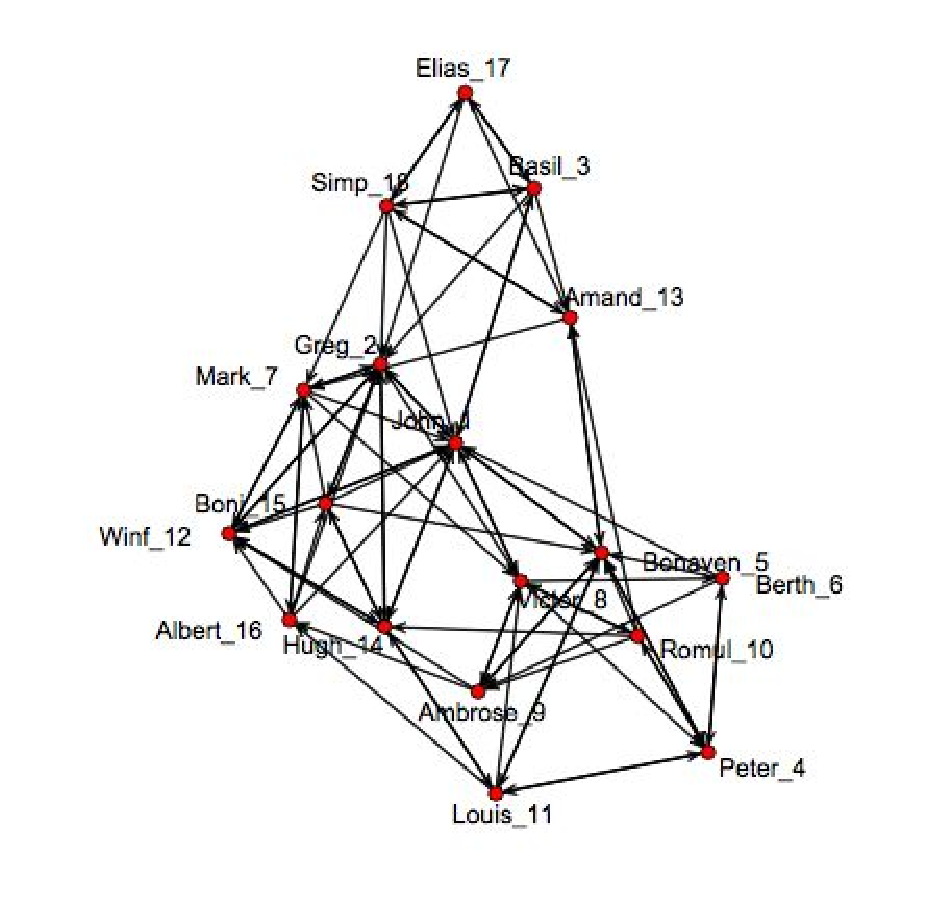
\includegraphics[width=5in, trim=0.2in 1in 0.3in .6in, clip=true ]{samplike} % l b r t
\end{center}
\caption[\citeauthor{Sampson}'s \citeyearpar{Sampson} monastery affinity network]
{\citeauthor{Sampson}'s \citeyearpar{Sampson} monastery affinity network.  \citeauthor{Sampson} collected data to define a ``liking" network among 18 monks 
in a New England monastery in the late 1960s.  Since ``liking" is a directional 
relation, the presence of a relation is depicted by an arrow rather than a line.  Data 
is available through and plotted using the \texttt{ergm} package \citep{ergm:R} in R.}
\label{F:Sampson}
\end{figure}

Stochastic network models were developed as early as 1959 in the seminal works of 
\citet{Gilbert} and \citet{Erdos}, resulting in a simple probabilistic model that is 
now referred to as the Bernoulli model or the Erd\"{o}s-R\'{e}nyi-Gilbert model.  Over 
the last forty years, more sophisticated stochastic network models have flourished;  
notable landmarks include the $p_1$ model of \citet{Holland:1981} which captures the 
reciprocal tendency of relationships in directed networks, and the $p^*$ model of 
\citet{Frank:1986} which describes the transitive tendency of relationships in 
undirected networks.  These models laid the foundation for the more general 
\emph{exponential random graph models (ERGM)}, a class of exponential family 
models that are now routinely used to model network data and are presented in 
detail in Section~\ref{S:ERGM examples}.\footnote{To be precise, they should
be called ``exponential \emph{family} random graph models", but apparently
this is too cumbersome.} 
% \citep{logit,Pattison:1999,Handcock:2006,introp*,advancesp*,recentp*,ergm,Morris:
%2008,Goodreau:2009,Goldenberg:2009}.

%\subsection{THE ISSUE -- DEPENDENCE}
At their core, stochastic network models attempt to describe whether or not a tie 
forms between each pair of actors in a group.
%  In the Florentine marriage network depicted in Figure~\ref{Padgett}, a model fit  
It has long been observed that relations, especially those involving humans, do not 
form in isolation; rather, they form in an interdependent manner.  Whether or not a 
relation forms between individuals $A$ and $B$ may very well depend on whether or not 
relations form between $B$ and $C$ and $C$ and $A$.  This has profound implications 
for the social scientist, necessitating a new ``network" perspective that recognizes 
the relational structures, such as a triangle of relations between actors $A$, $B$, 
and $C$, as factors in the analysis \citep[Chapter 1]{Wasserman:1994}.  This perspective has 
garnered increasing attention across different social and behavioral science 
disciplines over the last forty years, as evidenced by the rapid growth in publication 
of social network related papers \citep[Chapter 1]{Knoke:2008}.
% in the social science literature 
  
For the statistician, the network perspective means that the model should not break the 
network down into independent components, each containing two actors.
Instead, a good model will consider important relational structures in the observed network 
and clarify their contribution in shaping the global outcome.   
Accompanying the model must also be a computational algorithm to calibrate the model 
parameters to the network data.  
%In fact, this is the focus of our research.
In fact, writing down the expression for an uncalibrated ERGM turns out to be quite
straightforward; it is fitting the model
to data that is an open research problem and the focus of this dissertation.

Typically, parameter estimation for statistical models is done through the method of 
\emph{maximum likelihood} in which values for the parameters called \emph{maximum 
likelihood estimators (MLE)} that index the model to make the observed data most likely 
are calculated.
Many methodologies have been developed over the years to address the difficulties
in this process for exponential families
including Besag's \emph{pseudolikelihood} approach \citep{Besag:1974,Strauss:1990}, 
\citeauthor{Geyer:1992}'s \citeyearpar{Geyer:1992}
\emph{Markov chain Monte Carlo Maximum Likelihood} (MCMC-ML) approach, and 
\emph{stochastic approximation}.\footnote{Stochastic approximation has more general
applications in root finding, but is frequently used for parameter estimation.}
In fact, it was the absence of usable methodologies in parameter estimation that 
restricted earlier models like $p_1$ and $p^*$ to their simpler modeling capabilities.

%the simple expression belies the difficulties involved in fitting the model to data.
%In this paper, we describe further advances to these methodologies that address some of the
%pathologies researchers have encountered with these approaches.

Once model parameters are properly estimated, the fitted model can be used to simulate 
new random networks whose distribution retains essential characteristics of 
the observed network.  Researchers can then use this distribution 
to test hypotheses about the process of relationship formation.  
In this dissertation, we consider the ability to do statistical inference 
as the end goal of parameter estimation.  
Although we focus on an algorithm to find MLEs, our end goal  
is the maximum likelihood \emph{distribution},  which
can then be used to construct confidence intervals and evaluate hypotheses.

%Similarly, exponential random graph models have a deceptively simple form \eqref
%{E:ERGM} that belies the challenges involved in estimating the model parameters.  

%Network researchers have developed many descriptive statistics to capture 
%characteristics of a network.  For example, the number of ties going to a particular 
%actor is one measure of that actor's prestige in that network \citep{Wasserman:1994}.  

Finally, it should be noted that although problems from the social sciences provide much of the 
motivation for social network analysis and our research here, network models can in 
fact be applied to problems in a broad range of disciplines including political 
science, biology, epidemiology, and computer science and may be of interest
to business practitioners in the utility or transportation sectors.  
Actors often represent individuals but 
they may also represent entities like nation-states, protein molecules, airports, 
computers, or corporations.  The relation that connects actors 
is often friendship or actor $A$ 
``liking'' actor $B$, as in Sampson's monk data depicted in Figure~\ref{F:Sampson}, 
but the relation can be any kind, such as a business transaction or the 
Internet connectedness between computers.  Figure~\ref{F:ecoli} depicts the
\textit{Escherichia coli} gene transcription network among 423 mRNA molecules 
\citep*{Shen-Orr,Salgado}. This data was 
modeled with an ERGM by \citet*{Saul:2007} and again by \citet*{Hummel}.

\begin{figure}[h!]
\begin{center}
\includegraphics[width=5in, trim=0.2in 0.in 0.2in .in, clip=true ]{ecoli} % l b r t
\end{center}
\caption[\textit{E. coli} transcriptional regulation network of \citet{Shen-Orr}]{\textit{E. coli} transcriptional regulation network of \citet{Shen-Orr}.  Each node is an operon (a group of genes transcribed into a single mRNA molecule) and a directed edge from one node to another indicates 
that the first encodes the transcription factor that regulates the second.
Data is available through and plotted using the \texttt{ergm} package \citep{ergm:R} in R.}
\label{F:ecoli}
\end{figure}



%%%%%%%%%%%%%%%%%%%%%%%%%%%%%%%%%%%
\subsection{Why model networks?}
Before we step into a lengthy of discussion of how we model network data, it is 
worth reflecting upon the question of why network models are desirable or interesting.  We 
have already given one answer to this question in the context of the social scientist 
trying to differentiate between competing underlying forces that can shape the global 
structure of relationships: a network model will allow the researcher to 
identify if one or more actor specific variables and network structures 
contribute to the characteristic of the overall network.  That is, a good statistical 
model can see past noise in the data to
provide clarity of the underlying forces that shape the structure of an observed network
\citep*{Goodreau:2009}.   

In the context of epidemiology, a model for  
a \emph{contact network}, which is a network of the potential disease-causing ties between individuals, may be useful in understanding the general mechanism by which an epidemic can spread.  This may in turn help formulate an intervention strategy \citep*{Welch:2011}.
In computational biology, network models may be used to better understand the processes
by which proteins interact \citep*{Goldenberg:2009}.  
Some other applications of networks are the links between sites on the Internet
or the international relations between countries.  At its essence, 
a network is a conduit for flow, whether it be the flow of diseases, commodities, 
data, capital, or ideas, and network models can help us
 understand the mechanism of this flow \citep*{Kolaczyk:slides}.

\section{Exponential random graph models} \label{S:ERGM setup}
A network can be modeled as a random  $n \times n$ matrix $Y$, where $n$ is 
the number of actors.
Each entry $Y_{ij}$ in the random matrix $Y$ is itself a random variable representing 
a relation from actor $i$ to actor $j$, such that:
\[
	Y_{ij} = 
	\begin{cases}
		1 & \text{if a relation exists \textit{from} actor $i$ \textit{to} actor 
$j$ (notation: $i \to j$)}\\
		0 & \text{otherwise}
	\end{cases}
	\
\]
where $i$ and $j$ take values in $1, \ldots, n$, $i \neq j$.  
Note that $Y_{ij}$ take only values of $0$ or $1$, reflecting our restriction 
on networks to those with \emph{dichotomous} relations, that is, the relation between a pair 
of actors is either present or absent.  In addition, we do not allow  
$i \to i$ and always have $Y_{ii} = 0$.  In the special case that 
$Y_{ij} = Y_{ji}$ and thus the matrix $Y$ is symmetric, the network is referred to as an
\textit{undirected} network or graph, such as in the case of the Florentine marriage 
network depicted in Figure~\ref{F:Florentine}.  A network is \textit{directed} if it is 
not undirected, as in the case of monastery affinity network depicted in 
Figure~\ref{F:Sampson}.  

The exponential family random graph model (ERGM) commonly used in the network 
literature for $Y$ has probability mass function of the following form:
\begin{align}
	f_\eta(y) = P_{\eta}(Y=y) = \frac{1}{ \kappa( \eta) } e^{ \inner{ \eta, g(y)}  } \qquad y \in \YY, \label{E:ERGM}
\end{align}
where $g(y)$ is a $d$-vector of \emph{natural statistics}, $\eta$ is a 
$d$-vector of \emph{natural parameters}, 
$\inner{\fatdot,\fatdot}$ denotes the bilinear form
\begin{align*}
	\inner{ \eta, g } = \sum_{i=1}^d g_i \eta_i,
\end{align*}
and $\YY$ is the sample space of all possible networks with $n$ actors.
So that \eqref{E:ERGM} integrates to 1, $\kappa(\eta)$ is a normalizing constant such that
\begin{align}
   \kappa(\eta) &= \int e^{ \inner{ \eta, g(x)}  } \, d \mu(x) \label{E:kappa}
\end{align}
where $\mu$ is a measure on $\YY$.  In fact, \eqref{E:ERGM} is exactly the form of 
an exponential family distribution in \emph{canonical form} \citep[Chapter 1.4]{tpe}.  The only distinction that makes this an ERGM is that $\YY$ is specified to be the 
discrete state space of all possible network configurations.

We rely on many properties of exponential families.  Define 
the \emph{natural parameter space} $\Xi$ as the set of points
$\eta = (\eta_1, \ldots, \eta_d)$ that are parameter values indexing
distributions in the model.
An exponential family is \emph{full} if the natural parameter  space is
\begin{align} \label{E:paramspace}
   \Xi &= \{ \eta \in \RR^d : \kappa(\eta) < \infty \},  
\end{align}
 and \emph{regular} if, in addition, $\Xi$ is an open set.
%The exponential family is \emph{full} if the natural parameter space is \eqref
%{E:fullparam}, and \emph{regular} if, in 
%addition, $\Xi$ is an open set.  
We say an exponential family is \emph{minimal} if neither the natural parameter nor 
the natural statistic is concentrated on a hyperplane. 
Minimality guarantees that if an MLE, denoted $\etaMLE$, exists, 
it is unique \citep{Geyer:gdor}.


Define the \emph{cumulant} function as $c(\eta) = \log \kappa(\eta)$ and
denote the observed data as $\yobs$.  We can then express 
the log likelihood of \eqref{E:ERGM} as
\begin{align}
	\ell( \eta ) = \inner{ \eta, g(\yobs)} - c( \eta). \label{E:loglike}
\end{align}

The appeal of exponential families in the setting of complex dependence phenomena such 
as networks stems from their simplicity and maximum entropy property 
\citep{Jaynes:1978,Geyer:1992}.
By choosing statistics of interest on the data, one fully specifies a model that,
from a maximum entropy perspective, gives the 
most reasonable inference possible  derived solely from those statistics.  
Furthermore, exponential families have been 
well-studied \citep{Barndorff,Brown:1986} and utilized over the decades and have 
desirable properties such as the MLE uniqueness noted above.

%%%%%%%%% NETWORK STATISTICS
Ideally then, a network researcher need only specify relational structures of 
interest to define an ERGM.  
\citet*{Wasserman:1996, Pattison:1999, logit, introp*} describe many of 
the classical network statistics that one might include in the natural statistic vector 
$g(y)$.  In these works, the researchers' primary 
consideration in defining a network statistic is a relational structure's 
scientific interpretability.  
For example, in a directed affinity network, a sociologist may be 
interested in the propensity for individuals to form \emph{reciprocal} relations, where 
ties exist $i \to j$ and $j \to i$, or \emph{transitive} relations, where 
ties exist $i \to j$, $j \to k$, $i \to k$.  The statistics vector $g(y)$ 
that captures these can be defined by
\begin{align*}
	g(y) = \left ( \sum_{i<j} y_{ij}y_{ji}, \sum_{i \neq j \neq k} y_{ij}y_{jk}y_{ik} 
			\right )  
\end{align*}
where its components count the number of reciprocal and transitive relational 
structures in the network $y$.  
Such a model, with parameters appropriately calibrated to the affinity network, 
should then generate networks that exhibit a frequency of reciprocal and 
transitive relations similar to that of the observed data.
We will not discuss the merits of all the different network statistics 
here; in fact, there is essentially an unlimited number of potential network statistics.
What is important is that these statistics can be transparently calculated for a 
given network and the inclusion of them in $g(y)$, paired with their parameter 
components in $\eta$, allows the model \eqref{E:ERGM} to calculate probabilities of 
different global network outcomes $y$.  \citet*{ergm:userterms} 
even provide an interface for one to
customize and create her own network statistic of interest and model it in the 
\texttt{ergm} package in R.

%%%%%% RECENT NETWORK STATISTICS
More recently, \citet*{Handcock:2006, Hunter:2006, recentp*} developed
new network statistics with particular emphasis on the properties of 
the distributions as opposed to 
the scientific interpretability of the statistics themselves.
It had repeatedly been discovered that for some fitted models, the random networks generated
 from them did not at all resemble the observed network.  These new statistics
are intended to reduce the occurrence of such cases.
 A fairly complete description of these more recent network 
statistics is in \citet*{Morris:2008}.  We make use of one of these network statistics
in the example in Section~\ref{S:Example:FauxMagnolia}.
%We return to this issue in more detail in Section~\ref{S:Non-existent MLE}.
%In addition, the issue of model selection between competing models has not been 
%addressed though \citet{GOF} have begun making strides in this area.  Both of these 
%areas are active area of research.



%%%%%%%%%%%%%%%%%%%%%%%%%%%%%%%%%%%
\subsection{Intractable normalizing constant} \label{S:intractable}
We now return to the issue of why parameter estimation for ERGMs and 
similar exponential family models on discrete state spaces can be challenging.
Despite the tremendous appeal of the exponential family framework, one 
immediate problem is that the summation in \eqref{E:kappa} for the 
normalizing constant $\kappa(\eta)$ is over all possible 
networks in the sample space $\YY$ and can be prohibitively expensive to 
evaluate for networks of even moderate size.
For an undirected network with $n$ actors, there are $2^{{n\choose 2} }$ 
different possible networks in $\YY$.  Table~\ref{T:number graphs} shows how rapidly this number grows; 
unless dealing with networks of 9 actors or less, the likelihood function 
should not be directly evaluated.  See Appendix~\ref{A:Triangle count}
for our approach for counting simple network statistics in the 9-node network
relying on numerous tricks in data representation and computation.

\begin{table}[h!] 
\caption{Sample space size for undirected networks with different numbers of 
actors.}

\begin{tabular}{ccl} 
\hline 
Nodes & Possible Edges & Total Graphs \\ [1ex]
\hline
5 & ${5 \choose 2} = 10$ & $2^{10} = 1024$ \\ [1ex]
6 & ${6 \choose 2} = 15$ & $2^{15} = 32,768$ \\ [1ex]
7 & ${7 \choose 2} = 21$ & $2^{21} = 2,097,152$ \\ [1ex]
8 & ${8 \choose 2} = 28$ & $2^{28} = 268,435,456$ \\ [1ex]
9 & ${9 \choose 2} = 36$ & $2^{36} = 68,719,476,736$ \\ [1ex]
10 & ${10 \choose 2} = 45$ & $2^{45} = 3.518437\times10^{13}$ \\ [1ex]
\hline 
\end{tabular} \label{T:number graphs}
\end{table}

%%%%%%%%%%%%%%%%%%%%%%%%%%%%%%%%%%%
\subsection{Covariate data} \label{S:Covariate}
Information about a particular actor, say gender, can be incorporated as 
covariate data into the model with little difficulty.
Often, a social scientist looks to include such information because she is interested in
whether or not there is an \emph{assortative mixing} effect, that is, whether individuals of the same ``type" tend to make more relations with others of that type \citep{Goodreau:2009}.  
Suppose we wish to incorporate $p$ such exogenous attributes for our $n$-actor network.  
This information can be represented by an $n \times n \times p$ matrix $X$, whose 
$ijk$th element is the value of the $k$th attribute in the potential relation from actor
$i$ to $j$ \citep*{Fienberg:1981,ergm}.  We include such factors in our model 
of an adolescent friendship data set in Section~\ref{S:Example:FauxMagnolia}.

Like the other network statistics discussed, the statistics that comprise $X$ can 
be transparently calculated from data and hence included in the canonical 
statistics vector as $g(y, X)$,
with the canonical parameter vector $\eta$ lengthened accordingly.
The parameter estimation methodology is unchanged from before (so long as $p$ is not
excessively large), and while this greatly expands the
usefulness of ERGMs to the researcher, there are no new issues for us to consider
from a statistical modeling perspective.
Thus we will continue to use $g(y)$ instead of $g(y,X)$ for simplicity.  



%%%%%%%%%%%%%%%%%%%%%%%%%%%%%%%%%%%
\section{Examples of ERGMs} \label{S:ERGM examples}
We now review the classical Erd\H{o}s-R\'{e}nyi-Gilbert, $p_1$, and $p^*$ models to give both a sense of commonly used network structures as well as parameter estimation methodologies.

\subsection{Erd\H{o}s-R\'{e}nyi-Gilbert model} \label{S:Erdos}
The simplest example of an exponential random graph is the Erd\H{o}s-R\'{e}nyi-Gilbert 
model \citep{Erdos,Gilbert}, also referred to as a Bernoulli network model, which 
assumes that each actor forms a relation to every other actor independently with the 
same probability $p$ \citep{ergm}.  The ERGM can be expressed as
\begin{align*}
	P_{\eta}(Y=y) &= \frac{1}{\kappa( \eta) }e^{\eta g(y)}  \qquad y \in \YY, 
\end{align*}
where the only network statistic is a count of the number of edges for the directed network
\begin{align*}
%	g(y) = \frac{1}{N}\sum_{i \neq j} y_{ij},
	g(y) = \sum_{i \neq j} y_{ij}
\end{align*}
and the probability of a tie formation between any pair of actors is the same,
\begin{align*}
	p = P_\eta( Y_{ij} = 1) = \frac{e^{\eta}}{1+e^{\eta}}.
\end{align*}
%and thus the $Y_{ij}$ are mutually independent of one another.  
Then the log likelihood can be expressed as
\begin{align*}
	\ell(\eta) = \eta \sum_{i \neq j} y_{ij} - n(n-1) \log (1+ e^\eta).
\end{align*}

The MLE of $\eta$, $\etaMLE$, can be found analytically to be the logit of the 
fraction of ties that are present in the observed data set, 
\begin{align*}
	\etaMLE = \logit \left ( \frac{\sum_{i \neq j} y_{\textrm{obs}, ij}}{ n(n-1) } \right )
\end{align*}
where $n(n-1)$ is the number of possible ties in a directed network with $n$ actors.  
The MLE 
for $\eta$ is thus easily calculated from the observed data. The independence 
assumption, however, is too unrealistic for all but the simplest of cases; usually, 
a researcher is interested in modeling different probabilities of tie formations 
between actors.  Thus the Erd\H{o}s-R\'{e}nyi-Gilbert model may be most 
useful as a ``null'' model, though it is arguably too simple even for this.

%%%%%%%%%%%%%%%%%%%%%%%%%%%%%%%%%%%
\subsection{The $p_1$ model} \label{S:p1}
\citet{Holland:1981} made advances in relaxing this independence assumption  with 
their $p_1$ model.  They focused on two empirical observations from sociometric 
studies:
\begin{itemize}
\item Reciprocation: there tend to be a ``surplus" of mutual relationships in network 
data sets compared to a uniform distribution of directed relationships.
\item Stars: some individuals attract a surplus of choices compared to a uniform 
distribution of directed relationships.
\end{itemize}
\citeauthor{Holland:1981} then constructed a family of distributions with parameters 
to control the probability of observing different numbers of mutual relationships and 
stars.  
Focusing on the \textit{dyad}, the set of a pair of actors and the possible relations 
between them, as the basic building block, they proposed the following model:
\[
	P( Y = y ) = \frac{1}{ K( \rho, \theta, \{ \alpha_i \}, \{\beta_j \} )}\exp \left 
\{  \rho m(y) + \theta y_{++} + \sum_i \alpha_i y_{i+} +  \sum_j \beta_j y_{+j}\right 
\}
\]
subject to $\sum_i \alpha_i = \sum_j \beta_j = 0$, where
\begin{align*}
	\rho &= \text{``force of reciprocation" or mutuality parameter}\\
	m(y) &= \sum_{i \neq j} y_{ij}y_{ji}, \quad \text{total number of mutual relationships 
in $y$}\\
	\theta &= \text{``density" or overall choice effect parameter}\\
	y_{++} &= \sum_{i \neq j} y_{ij}, \quad  \text{total number of relations in $y$}\\
	\alpha_i &= \text{``productivity" or ``expansiveness" effect parameter for node $i
$}\\
	y_{i+} &= \sum_{j} y_{ij}, \quad  \text{``out-degree" for node $i$ in $y$}\\
	\beta_j &= \text{``attractiveness" or ``popularity" effect parameter for node $j$} 
\\
	y_{+j} &= \sum_{i} y_{ij}, \quad  \text{``in-degree" for node $j$ in $y$}\\
	K &= \text{normalizing constant}
\end{align*}

By defining new dyad random variables, $D_{ij} = (Y_{ij}, Y_{ji} )$, \citeauthor
{Holland:1981}  showed that with some algebraic manipulation, the form of the model above 
can be viewed as a log-linear model with independent dyad random variables 
$D_{ij}$.  This makes it possible to use a standard logistic regression to calculate MLEs of the parameters.

The statistical independence at the dyad level, however, means that this model will 
not capture triangular tie configurations (or anything more complicated) in which dyads are dependent.  Also, to 
reduce the number of parameters, the model assumes $\rho_{ij} = \rho$ and $\theta_{ij} = \theta$, meaning that the 
tendency towards reciprocity and forming relations is assumed to be the same across all actors.  This example 
illustrates how the parameter estimation methodology limits the scope of the model and 
what types of behavior it can capture.  

%%%%%%%%%%%%%%%%%%%%%%%%%%%%%%%%%%%
\subsection{Markov graph model}
\citet{Frank:1986} relaxed the independence assumption further with the implementation 
of \textit{Markov dependence} in which two dyads are independent, conditional on the 
rest of the graph, when they do not share a node.  The model uses only three 
configurations in an undirected network, expressed as:
\[
	P( Y = y ) = \frac{1}{K( \theta, \sigma, \tau)}\exp 
				\left \{ \theta L + \sigma S + \tau T	\right \} 
	\]
where
\begin{align*}
	\theta &= \text{edge parameter} \\
	L &= \sum_{i < j} y_{ij}, \quad \text{total number of edges} \\
	\sigma &= \text{2-star parameter, propensity for individuals to have connections 
with two actors} \\
	S &= \sum_{i < j < k} y_{ij}y_{ik}, \quad \text{total number of 2-stars ($i \leftrightarrow j$, $i \leftrightarrow k$) }\\
	\tau	&= \text{Triangle parameter, represents clustering} \\
	T &= \sum_{i < j < k} y_{ij}y_{jk}y_{ik}, \quad \text{total number of triangles ($i \leftrightarrow j$, $j \leftrightarrow k$, $i 
\leftrightarrow k$)}
\end{align*}
None of the above parameters have subscript indices, reflecting the simplification 
from a \textit{homogeneity} assumption where parameters are equated if the 
network structures are the same ignoring the labels on the nodes (also called \textit
{isomorphic} configurations.  In fact, this is the same simplification \citeauthor{Holland:1981} employ for the $\rho$ and $\theta$ parameters in their $p_1$ model).

The model is the first to break dyad independence, made possible by \citeauthor{Frank:1986}' methods of parameter estimation.  In particular, \citeauthor{Frank:1986} ran
Markov chain Monte Carlo simulations of the model at multiple values for a parameter 
to determine which fit the data best.  The authors also obtained 
\emph{maximum pseudolikelihood estimators (MPLE)} from a standard logistic 
regression (we discuss the pseudolikelihood approach in Section~\ref{S:pseudolikelihood}) 
and observed that the MPLEs are close to those they arrived at from their rigorous simulations.   \citeauthor{Frank:1986} seem to conclude that MPLEs are generally quite acceptable.  


%%%%%%%%%%%%%%%%% SECTION %%%%%%%%%%%
\section{ERGM parameter estimation}
Exponential random graph models have a deceptively simple form \eqref
{E:ERGM} that belies the challenges involved in model parameter estimation.
As discussed in Section~\ref{S:intractable}, the difficulties
arise from a normalizing constant \eqref{E:kappa} which may involve 
a summation over an astronomical number of terms.
In this section, we discuss commonly used parameter estimation methods
used for exponential families with complex dependence like ERGMs.  All approaches avoid evaluating the likelihood function directly but have properties that we
find undesirable.   The methods are aided by a strictly concave 
log likelihood function (see Section~\ref{S:Expfam theory}) and thus there is
no worry about local maxima. There can be at most one local maximum, which (if it
exists) is the global maximum.
  
%These provide the backdrop for the new algorithm we propose in this paper.

%However, even with increasingly sophisticated simulation methods, finding MLEs for 
%ERGMs can be problematic in two ways:
%\begin{enumerate}
%\item The methodology used to find MLEs fails due to a shortcoming in the methodology 
%itself.  That is, an alternative approach might yield parameter estimates resulting in 
%a perfectly good model.
%
%\item The model itself is specified in such a manner so that it can be classified as 
%\emph{degenerate}, a term first applied to ERGMs by \citet{Handcock:Degeneracy} and 
%further clarified by \citet{Rinaldo:2009} to refer to instances where
%\begin{enumerate}
%\item Random graphs generated from the fitted model lack variability, often only 
%giving rise to unrealistic graphs, usually empty or complete (or nearly complete).
%\item the MLE does not exist.
%\item The fitted model makes the observed network highly unlikely.
%\end{enumerate}
%\end{enumerate}
%The two issues are related; for example, if the MLE does not actually exist, then 
%commonly used algorithms sent to find it will surely fail, or worse, return values 
%that the user may then treat as correct.   The issue is significant enough to be a 
%barrier to the use of ERGMs \citep{advancesp*}.



\subsection{Maximum pseudolikelihood method} \label{S:pseudolikelihood}
As mentioned in Section~\ref{S:p1}, \citet{Frank:1986} successfully applied 
the maximum pseudolikelihood method to social network models, a method first used in lattice systems in plant biology \citep{Besag:1974,Besag:1975}.  \citet{Strauss:1990} further justified the use of 
maximum pseudolikelihood estimators (MPLE) as reasonable approximations for MLEs in 
social network models.  \citet*{Wasserman:1996, Pattison:1999, logit} leaned on this 
result to broaden the scope of network models, allowing 
for any combination of network structures to be considered.  The result is \eqref{E:ERGM},
the more general form of the ERGM that is currently used.

The method of maximum pseudolikelihood finds the values for the parameters that 
maximize the \textit{pseudolikelihood function} for the observed 
data set, which can be constructed from the densities of $Y_{ij}$ 
conditional on the rest of network, denoted by $f_{Y_{ij}}( y_{ij} \mid \textrm{rest})$.
The pseudolikelihood function $PL(\eta)$ is defined to be the product of these densities,
\begin{align}
	PL(\eta) = \prod_{i \neq j}f_{Y_{ij}}( y_{ij} \mid \textrm{rest}), \label{E:PL}
\end{align}
and in general is different than the likelihood function.

Define the vector of \textit{change statistics} $\delta_g(y)_{ij}$ to be
\begin{align*}
	\delta_g(y)_{ij} = g(y_{ij}^+) - g(y_{ij}^-)
\end{align*}
where $y_{ij}^+$ and $y_{ij}^-$ represent networks with $y_{ij} = 1$ and $y_{ij} = 0$, 
respectively, while leaving the rest of the network as $y$.  Thus $\delta_g(y)_{ij}$ 
is the change in $g(y)$ when $y_{ij}$ changes from 0 to 1.
The conditional distribution of $Y_{ij} \mid \textrm{rest}$ for an ERGM is then a Bernoulli 
distribution with log odds
\begin{align}
	\log \left ( \frac{P( Y_{ij} =1 \mid \textrm{rest} ) }
				 	 { P( Y_{ij} =0 \mid \textrm{rest} ) } \right ) 
					 			= \eta^T \delta_g(y)_{ij}. \label{E:logodds}
\end{align}
%(See \citet*[Appendix]{Composite} for a derivation of \eqref{E:logodds}.)  
The form of \eqref{E:logodds} in the context of \eqref{E:PL} naturally lends
itself to the use of logistic regression to find values of $\eta$ that
maximize $PL(\eta)$.  These values of $\eta$ are called the maximum pseudolikelihood estimators.

In the case where the $Y_{ij}$ are in fact mutually independent, the MPLEs will equal the MLEs.  
\citet{Strauss:1990} show that in 
many cases with dyad dependence, MPLE still yield reasonable approximations of the 
true MLEs.  

However, \citet*{Geyer:1992, Snijders:2002, introp*, Duijn:2009} demonstrated that 
the pseudolikelihood approach can produce very misleading results 
when dependence is strong.  
\citet*{Composite} showed that the pseudolikelihood approach can be 
improved upon in a generalization 
called the \emph{composite likelihood} approach; this method is identical
to pseudolikelihood except that the conditional distributions used to build the \emph{composite likelihood function}---analogous to the pseudolikelihood function \eqref{E:PL}---are for multiple 
ties rather than a single tie.
%Nevertheless, researchers now avoid citing parameter estimates based on these approaches.
\citet{Hummel} raised two additional issues with the pseudolikelihood approach, 
which also apply to the composite likelihood approach. 
The first is that this approach requires
an actual network $\yobs$ from which to derive the MPLE, as opposed to a network
statistics $g(\yobs)$ which may be some vector of theoretical interest to 
which one would like to fit an ERGM.  Thus given a $g(\yobs)$, one would then
need to take the extra step of finding a $\yobs$ that matches this vector of
interest.  The second point is that there are several networks that
yield the same $g(\yobs)$.  Because ERGMs depend only on $g(\yobs)$ and not $\yobs$,
these will all yield the same MLE.  However, there is no guarantee that they will yield the same MPLE.
Network software packages such as \texttt{statnet} \citep*{statnet:R} in the R 
platform now overwhelmingly use MLE methods, using MPLEs only as starting points
as in the example in Section~\ref{S:Example:FauxMagnolia}.

%%%%%%%%%%%%%%%%%%%%%%%%%%%%%%%%%%%%%%%%%%%%%%%%%
\subsection{Newton-Raphson}
Newton-Raphson is one of the most commonly used root-finding algorithms
in optimization, attractive
for its speed of convergence.  It relies on iterated updates of a root 
function, which in our setting is the gradient of the log likelihood, $\nabla \ell(\eta)$.  
The algorithm also requires the Hessian matrix $\nabla^2 \ell(\eta)$ and has updates 
of the following form:
\begin{align}
	\eta_{k+1} = \eta_k - \left[ \nabla^2 \ell(\eta_k) \right ]^{-1} \nabla \ell(\eta_k).
\end{align}
The algorithm may fail to 
converge when the initial $\eta_k$ is far from the solution.  However,
when Newton-Raphson does converge, it converges extremely fast, 
where the number of accurate digits roughly doubles at each step.

We use a stochastic version of Newton-Raphson in Section~\ref{S:Example:Ising} where 
we wish to calculate MLEs for comparison purposes and are able to start the algorithm from the known true parameter value.
Both $\nabla \ell(\eta)$ and $\nabla^2 \ell(\eta)$ can be approximated using MCMC 
 \citep{Penttinen:1984}.
%%%%%%%%%%%%%%%%%%%%%%%%%%%%%%%%%%%%%%%%%%%%%%%%%
\subsection{Markov chain Monte Carlo maximum likelihood} \label{S:MCMC-MLE}
\citet{Geyer:1992, Corander:1998, Snijders:2002} developed Markov chain Monte Carlo 
(MCMC) methods to approximate the MLE of an exponential family.  Of these, \citeauthor
{Geyer:1992}'s Markov chain Monte Carlo-maximum likelihood estimator (MCMC-MLE) method 
appears to have become the standard approach in the network literature 
\citep{Hunter:2006, Handcock:2006, GOF} and is the default algorithm in 
the \texttt{statnet} suite \citep{statnet:R} in the R platform for network models.  
An additional attraction of MCMC-MLE is that it provides a way to give accurate error 
estimates \citep{Geyer:1994,Hunter:2006}.

The MCMC-MLE approach is theoretically guaranteed to converge to the MLE if it exists.  
Rather than maximizing the log likelihood \eqref{E:loglike}
with respect to $\eta$, \citeauthor{Geyer:1992} consider 
the log of the likelihood ratio $r( \eta, \eta^0 )$, where $\eta^0$ 
is fixed at a known value,
\begin{align}
 r( \eta, \eta^0 ) &= \ell( \eta ) - \ell( \eta^0 ) \notag \\ 
				  &= \inner{ \eta - \eta^0, g(\yobs)} - \log \left [ \exp \bigl( c(\eta) - c(\eta^0) \bigr) \right ].\label{E:r}
\end{align}
The value of $\eta$ that maximizes an
approximation of $r( \eta, \eta^0 )$ is then a good estimate of the MLE, 
assuming it exists.  In order to avoid evaluating the problematic normalizing constant,
this approach equates the ratio of normalizing constants 
$\exp \left (  c(\eta) - c(\eta^0) \right )$ to an expectation 
using \eqref{E:kappa} as follows:
\begin{align}
	\exp \left (  c(\eta) - c(\eta^0) \right ) &= \frac{ \int \exp \bigl ( \inner{ \eta, g(x) }\bigr ) \, d\mu(x) }{ \kappa(\eta^0)  } \notag \\
	&= \frac{ \int \exp \left ( \inner{ \eta - \eta^0, g(x)} + \inner{ \eta^0, g(x)} \right ) \, d\mu(x)  }{ \kappa(\eta^0) } \notag \\
	&= \int \exp \left( \inner{\eta - \eta^0, g(x} \right ) \frac{ e^ { \inner{ \eta^0, g(x)} } }{ \kappa(\eta^0) } \, d\mu(x) \notag \\
	&= \E_{\eta^0} \exp \left( \inner{ \eta - \eta^0, g(Y)}  \right ) . \label{E:E eta0}
\end{align}
While we choose $\eta_0$ to index a distribution 
in the same family as the one indexed by $\eta$ in \eqref{E:E eta0}, this can be generalized \citep{Geyer:1996}.  We keep this restriction here
because the MCMC samplers in the \texttt{statnet} package only simulate from distributions in the model and so can only use this formula.
          
%It should be noted that while we choose $\eta_0$ to index a distribution from the same
%family as the one indexed by $\eta$ in \eqref{E:r}, in fact its distribution need 
%only have the same support \citep[pp.~251--256]{Geyer:1996}.
%We will continue with this restriction not only for simplicity but also because this is how
%the methodology is implemented for ERGM parameter estimation in the \texttt{statnet} package
%\citep{statnet:R} in R.

By the Markov chain strong law of large numbers \citep[Theorem 17.0.1]{Meyn:2009}, 
%(or Birkhoff ergodic theorem), 
this expectation can be approximated by the sample mean for large Monte Carlo sample 
size,
\begin{align*}
	\frac{1}{m} \sum_{i=1}^{m}\exp \left ( \inner{ \eta - \eta^0,g(Y_i)} \right )
\end{align*}
where $Y_1, \ldots, Y_m$ are draws from the exponential family distribution with 
parameter $\eta^0$.  This sample can be generated using MCMC 
methods such as the Metropolis-Hastings algorithm \citep{Geyer:2011}, which
is typically used for ERGMs.

Thus \eqref{E:r} can be approximated by
\begin{align}
\hat{r}_m( \eta, \eta^0 ) &= \inner{ \eta - \eta^0, g(\yobs)} - \log 
	\left [ \frac{1}{m} \sum_{i=1}^{m} \exp \left ( \inner{ \eta - \eta^0, g(Y_i)} \right ) \right ] 
%	\left [ \frac{1}{m} \sum_{i=1}^{m} e^{  \inner{ \eta - \eta^0, g(Y_i)} } \right ] 
	\label{E:r_hat}
\end{align}
and for any fixed $\eta$
\begin{align*}
	\hat{r}_m( \eta, \eta^0 ) \to r( \eta, \eta^0 ) \text{ a.s. as $m \to \infty$}.
\end{align*}
This holds for all $\eta$ in any countable set and thus for some dense set.
If we call $\hat{\eta}_m$  the maximizer of \eqref{E:r_hat} and assume that the MLE 
$\etaMLE$ exists, \citeauthor{Geyer:1992} show that 
\begin{align*}
	\hat{\eta}_m \to \etaMLE, \quad \text{a.s.}
\end{align*}
 whenever the Markov chain is ergodic. 
 
This approach has been shown in practice to be sensitive to initial parameter 
values when used without the trust region methodology recommended in \citet{Geyer:1992}, 
and the algorithm may require enormous---sometimes infeasibly large---Monte Carlo sample sizes 
when the starting value $\eta^0$ is far from the MLE \citep{ergm}.  
In addition, \citeauthor{Geyer:1992} recommend iterating the algorithm several times, 
where each successive maximizing value will be closer to $\etaMLE$ than the previous
if sample sizes are sufficiently large.  At the 
time of this writing, the MCMC-MLE routine in \texttt{statnet} uses by default 10,000 
Monte Carlo samples spaced 100 samples apart and a maximum of three iterations, using the 
MPLE as the initial value for $\eta^0$ \citep{statnet:R}.  
Improvement of the MCMC-MLE approach is an active area of research \citep*{Bartz}.
An extension of this method by \citet{Hummel} is discussed in the next section.

\citet{ergm} illustrate the practical difficulty associated with a poor initial 
value in the MCMC-MLE algorithm with Sampson's monastery data set depicted in 
Figure \ref{F:Sampson}.  The 
observed network $\yobs$ is directed with 18 actors and 88 ties present out of $18 \cdot 17=306$ possible 
ties.  To illustrate the issue, \citeauthor{ergm} use the Erd\H{o}s-R\'{e}nyi-Gilbert model 
described in Section~\ref{S:Erdos} with network statistic $g(y)$ equal to the total number of 
edges present.  As noted earlier, the true MLE is equal to 
\begin{align*}
	\etaMLE = \logit\left( \frac{g(\yobs)}{n(n-1)}\right) = \logit \left( \frac{88}{306}\right ) = -0.9072.
\end{align*}
  
When $\eta^0$ is chosen to be $1$, however, \citeauthor{ergm} show that it is
extremely difficult for the algorithm to attain the MLE in a single iteration of 
the MCMC-MLE algorithm.  
For this value of $\eta$, the model dictates that each of the 306 possible edges occur independently with probability $p = \frac{1}{1+e^{-\eta}} = \frac{1}{1+e^{-1}} = 0.731$.   
This is a very high probability relative to the sparsity of relations in the observed data 
set, which suggest a much smaller probability of tie formation of $88/306= 0.288$.  
In fact, the probability of obtaining fewer than 88 ties for the $\eta=1$ model is nearly zero at $2.3 \times 10^{-59}$, calculated using a binomial distribution with $n=306$, $p =0.731$.  

\begin{figure}[h!]  
\begin{center} 
%{\includegraphics[width=2.95in]{mcmc-mle1}}
%{\includegraphics[width=2.95in]{mcmc-mle-1}}
{\includegraphics[width=3.2in]{mcmc-mle1-bw}}
{\includegraphics[width=3.2in]{mcmc-mle-1-bw}}
\end{center} 
\caption[Log likelihood ratio approximations in Sampson's monastery example]{Log likelihood ratio approximations in Sampson's monastery example.  Top: $\eta^0 = 1$, Bottom: $\eta^0 = -1$. Solid lines are exact log likelihood ratios $\ell(\eta) - \ell(\eta^0)$, dotted lines are the 
approximation by \eqref{E:r_hat} using 100,000 MCMC samples.  
MLE is at $-0.9072$.
Data for plots are produced using code accompanying \citet{Hummel}.} 
\label{F:MCMC-MLE}
\end{figure} 

The MCMC-MLE algorithm maximizes the approximated log 
likelihood ratio \eqref{E:r_hat}.  However, the first derivative of $\hat{r}(\eta,\eta^0)$ with respect
to $\eta$ shows that if the MCMC sampler is unable to generate any $g(Y)< g(\yobs)$, 
the derivative of 
\eqref{E:r_hat} will be strictly negative, resulting in $\hat{r}(\eta,\eta^0)$ with no
maximum.  This is depicted by the dotted-line in Figure \ref{F:MCMC-MLE} (top).  
The problem is not present when the initial value is close to the true MLE, such as 
when $\eta^0 = -1$; the corresponding $r(\eta,\eta^0)$ and $\hat{r}(\eta,\eta^0)$ 
functions are depicted in Figure \ref{F:MCMC-MLE} (bottom).  With the default three 
iterations of MCMC-MLE in the \texttt{statnet} package, the algorithm 
starting with $\eta^0 = 1$ is only able to obtain an estimate for $\eta$ as 
small as $\eta = -0.364$.  With 10 iterations, it does in fact 
arrive at the MLE of $-0.907$.




%%%%%%%%%%%%%%%%%%%%%%%%%%%%%%%%%%%%%%%%%%%%%%%%% 
\subsection{Steplength MCMC-MLE} \label{S:Hummel}
\citet{Hummel} expanded the range for which iterated MCMC-MLE will converge by
making incremental updates in $\eta$ towards $\etaMLE$ possible at each iteration.  
As noted in the 
previous example with 
Sampson's monastery data, $\hat{r}(\eta,\eta^0)$ 
will have no maximum if $g(\yobs)$ is outside the range of MCMC samples.  
\citeauthor{Hummel}'s approach involves 
replacing $g(\yobs)$ with a value $\hat{\xi}_1$ close to $g(\yobs)$ but within
the range of the current model's MCMC samples.
This makes it possible to maximize $\hat{r}(\eta,\eta^0)$ and update $\eta^0$,
with the resulting $\eta$ necessarily closer to $\etaMLE$.

The approach is effective for Sampson's monastery example discussed, and was also applied
to the \emph{E. coli} biological network data of \citet{Shen-Orr} when 
starting from the MPLE.  Care is needed in finding a $\hat{\xi}_1$ that is inside
the range of the current model. In addition, if $\eta_0$ is very far from $\etaMLE$, it is 
not clear that the steps taken by this approach will be large enough to traverse
the distance between $\eta^0$ and $\etaMLE$ in any reasonable amount of time.



%\subsection{Generalization to exponential families}
%
%The algorithm and approaches we present here are generally applicable to all regular 
%exponential families on finite state spaces, including ERGMs.  Thus we present the 
%background theory at the higher level of exponential families though we will return to 
%ERGMs in our most complicated applications.

    
%%%%%%%%%%%%%%%%%%%%%%%%%%%%%%%%%%%%%%%%%%%%%%%%%
\subsection{Stochastic approximation}

Variations on the Robbins-Monro \emph{stochastic approximation} (SA) algorithm 
\citep{Robbins-Monro} have been applied to find the MLE in similar contexts: 
\citet{Younes:1988,Younes:1989,Moyeed:1991,Gu:2001}
applied MCMC stochastic approximation to spatial models and \citet{Snijders:2002} to 
ERGMs.
%Our approach shares a similar recursive mechanism with SA, so we will describe this 
%method further.  
SA procedures for finding the MLE of a parameter $\eta$ generate iterated estimates 
$\eta_k$ to find the 
root of a gradient function $h(\eta)$:
\begin{align} \label{E:eta SA update}
	\eta_{k+1} = \eta_k + \alpha_k U_k,
\end{align}
where $\alpha_k$ is a step size and is typically a member of a decreasing sequence of 
positive numbers, and $U_k$ is a 
random variable from the distribution specified by $\eta_k$ that noisily estimates the 
gradient function $h(\eta_k)$.  

Restrictive conditions are required of $\alpha_k$ and $U_k$ to establish convergence 
of the sequence $\eta_k$.  
In Robbins-Monro SA \citep{Robbins-Monro}, the step size $\alpha_k$ must be a sequence 
of positive constants 
that satisfies 
\begin{align*}
	\sum \alpha_k^2 < \infty
%	\sum \alpha_k = \infty, \qquad \sum \alpha_k^2 < \infty.
\end{align*}
for which the choice of
\begin{align} \label{E:SA step size}
	\alpha_k = \frac{A}{B + k}
\end{align}
 is commonly used, where $A$ and $B$ are constants that must be specified by the user.  
This specification requires experimentation and care: there can be significant 
variation in performance depending on choice of these constants. 
Some recent research show that sequences that go to 0 
slower than $1/k$ can result in an improved rate of convergence,  where rate of
convergence is measured by the asymptotic covariance of the normalized estimates about 
their limit point \citep[Chapter 11]{Kushner:1997}.
%Regardless of the exact form, there is no guarantee the likelihood function will 
%increase at each update. 

The conditions on $U_k$ are more restrictive.  Popular approaches include constraining 
the sequence of estimators $\eta_k$ to a compact set specified \emph{a priori}, 
or assuming that the noise component of $U_k$ be a martingale 
difference sequence.  As commonly observed \citep*{Chen:2002,Andrieu:2005,Liang:2010} 
these may be 
difficult to satisfy in practice.  
See \citet{Andrieu:2005,Liang:2010} for recent developments that impose less 
restrictive conditions using truncated 
updates.

An issue for any recursive search algorithm is the 
choice of starting point.  It is 
often the case that algorithms are good at finding the MLE when the starting point is 
close to it, but of course the 
location of the MLE is unknown.  For any exponential family with bounded support, 
Fisher information 
becomes singular as the canonical parameter $\eta$ goes to $\infty$ \citep*{Rinaldo:2009}.
Hence methods which rely on 
the Fisher information matrix may fail when the starting point for $\eta$ is far from 
the MLE \citep{Younes:1989,Gu:2001}.
Of course, one may try different starting points until a ``good'' one is found, but 
this comes with no theoretical guarantees and can be cumbersome in practice.

%%%%%%%%%%%%%%%%%%%%%%%%%%%%%%%%%%%%%%%%%%%%%%%%%
\subsection{Summary of parameter estimation methods}
Tables~\ref{T:Compare estimation} and \ref{T:Compare MCMCestimation} summarize the advantages and disadvantages of the exact and MCMC parameter estimations discussed.  
All methods assume that the MLE exists before the search algorithm is applied and that
the log likelihood is strictly concave.

\begin{table}[h!] 
\caption[Comparison of exact parameter estimation methods]{Comparison of exact parameter estimation methods. MPLE=Maximum pseudolikelihood estimator, Newton=Newton-Raphson.\\}

\begin{tabular}{|c|l|l|}
\hline 
Method & Appeal & Drawbacks \\ [1ex]
\hline
\multirow{2}{0.5in}{MPLE}		
& 	\textbullet \, Simplicity 				  	& \textbullet \, Maximizes pseudolikelihood, not\\
& 	\textbullet \, Speed, via logistic regression 	&  likelihood \\ [1ex] % \textbullet \, MPLE behavior not well understood \\ [1ex]
\hline
\multirow{3}{0.5in}{Newton}
& 	\textbullet \, Converges rapidly when it & \textbullet \, Highly sensitive to starting point\\	
& converges & \textbullet \, Requires second derivative matrix and \\ 
& 	 	&  its inverse\\ [1ex] 
%\hline
%\multirow{3}{0.5in}{SA} 		
%& 	\textbullet \, Simple updates 				& \textbullet \, Requires trial-and-error calibration  \\			& 	\textbullet \, Theoretically guaranteed to		& \textbullet \,  May converge too slowly to be practical   \\
%& 	converge to MLE with proper  & \\
%& 	setup  & \\[1ex]
\hline 
\end{tabular} 
\label{T:Compare estimation}
\end{table}

\begin{table}[h!] 
\caption[Comparison of MCMC parameter estimation methods]{Comparison of MCMC parameter estimation methods. MCMC Newton=MCMC Newton-Raphson,
MCMC-MLE=Markov chain Monte Carlo-maximum likelihood estimator, 
step MCMC-MLE=steplength MCMC-MLE,
MCMC SA=stochastic approximation.\\}

\begin{tabular}{|c|l|l|}
\hline 
Method & Appeal & Drawbacks \\ [1ex]
\hline
\multirow{3}{0.5in}{MCMC Newton}
& 	\textbullet \, Converges rapidly when it  & \textbullet \, Requires calculation of second derivative \\
& 	converges 	& matrix and its inverse, which typically  \\	
&				&  requires staring point very close to solution \\[1ex]
\hline
\multirow{3}{0.5in}{MCMC-MLE}
& 	\textbullet \, Theoretically guaranteed to   	& \textbullet \, Highly sensitive to starting point \\ 
& 	converge to MLE 					& \textbullet \, May require enormous MC sample sizes\\ 
&				& \textbullet \, May require several iterations\\ [1ex]
\hline
\multirow{3}{0.5in}{step MCMC-MLE}
& 	\textbullet \, Theoretically guaranteed to   	& \textbullet \, Sensitive to starting point \\ 
& 	converge to MLE 					& \textbullet \, Requires setup expertise\\ 
& \textbullet \, Increased range 		& \textbullet \, May require several iterations\\ [1ex]
\hline
\multirow{3}{0.5in}{MCMC SA} 		
& 	\textbullet \, Simple updates 				& \textbullet \, Requires trial-and-error calibration  \\			& 	\textbullet \, Theoretically guaranteed to		& \textbullet \,  May converge too slowly to be practical   \\
& 	converge   & \textbullet \,Convergence conditions not easily  \\
& 	  & implemented in practice \\[1ex]
\hline 
\end{tabular} 
\label{T:Compare MCMCestimation}
\end{table}
%%%%%%

%\begin{figure}[h]
%\begin{center}
%\includegraphics[width=4.5in]{mck.pdf}
%\end{center}
%\caption{What I got out of case studies.}
%\label{F:mck}
%\end{figure}

%%%%%%%%%%%%%%%%%%%%%%%%%%%%%%%%%%%%%%%
\section{Non-existent MLEs in exponential families} \label{S:Non-existent MLE}
Parameter estimation via maximum likelihood for exponential family models with 
complex dependence---already a 
challenging problem because the likelihood function may be computationally 
infeasible---is further obfuscated by the possibility that the MLE
may not exist.  
In such a case, the strictly concave likelihood function is
increasing in some direction of the parameter space, called a 
\emph{direction of recession}, so that the MLE is actually off ``at infinity".
The theoretical background 
for this situation has been understood for many years 
\citep{Barndorff,Brown:1986}: MLE existence is a
geometric problem relating to properties of the \emph{convex support} of the model,
which is  the smallest closed convex set 
that the contains the natural statistic \citep{Geyer:gdor}.  
The MLE does not exist in the conventional sense if the 
observed data is in the relative boundary of this 
convex support (see Section~\ref{S:MLE existence}).
When this occurs, 
it may exist in the \emph{Barndorff-Nielsen completion} of the family.
Before this dissertation, there have been no 
computationally convenient approaches to handling this issue for social network models
and other discrete exponential family models with complex dependence.

\citet{Geyer:1992} separated the search for the MLE of an exponential family model
with complex dependence into a two-phase algorithm, 
where phase I determines whether or not an MLE exists in the conventional 
sense via linear programming, and phase II finds the MLE when it exists.
\citeauthor{Geyer:1992}'s MCMC-MLE method discussed in Section~\ref{S:MCMC-MLE} corresponds to phase II of
this approach.
In the special case of generalized linear models including logistic regression and contingency 
tables, \citet{Geyer:gdor} outlines a methodology to detect non-existent MLEs and construct 
one-sided confidence intervals for the natural parameters.
The approach applies linear programming to the polyhedral convex support of 
the model to determine the \emph{face} of the convex support 
in which the observed data lies.  
This face in turn defines the convex support for a new exponential family for which the MLE 
does exist and can be found using conventional methods (see Section~\ref{S:LCM}).
The linear programming 
functionality has been implemented in the R package \texttt{rcdd} \citep*{rcdd:R}.

\citet*{Handcock:degeneracy, Rinaldo:2009} focus on problematic instances of parameter 
estimation for ERGMs, which are loosely referred 
to as \emph{degeneracy}.  Strictly speaking, a distribution in an exponential
family is degenerate when it concentrates the distribution of the natural statistic
on a hyperplane.  If the family is minimal, this occurs if and only if the MLE does not exist in the conventional sense.  This in turn means that the observed
data lies on the relative boundary of the convex support.  \emph{Near} degenerate  
means that the observed data lies nearly on this relative boundary.
However, the terms degeneracy and near degeneracy
are now invoked if there are undesirable behaviors of the fitted model or 
in the model fitting process itself
\citep{Handcock:degeneracy,advancesp*,recentp*,statnet-tutorial}.
We will only use the terms for their original meanings here.   

\begin{figure}[h!]
\centering
\includegraphics[width=5in]{Figures/g9-hull-bw}
\caption[Sample space of two-dimensional statistic for 9-node network model]{Sample space 
of two-dimensional statistic for 9-node network model.  \citet{Rinaldo:2009} focused
on edge and triangle statistics.  The shading of a point corresponds to 
the frequency of graphs with that network statistic.  
The convex support is the gray, sail-shaped polytope.  Points on the 
boundary have an outlined circle and extreme points are square.}
\label{F:g9-hull}
\end{figure}

To better understand ERGM pathologies, \citeauthor{Handcock:degeneracy,Rinaldo:2009}
study small networks with 7 and 9 nodes.  At these sizes, it is still 
possible to explicitly evaluate the likelihood function \eqref{E:ERGM} and thus 
find MLEs using standard numerical optimization routines.  
As in \citep{Geyer:gdor}, the emphasis is on the geometric properties of the 
polyhedral convex support of the model;
the convex support for the 9-node ERGM with a two-dimensional network statistic of
edges and triangles
studied by \citeauthor{Rinaldo:2009} is depicted in Figure~\ref{F:g9-hull}.
\citeauthor{Rinaldo:2009} showed that the normal cones (see Section~\ref{S:Convex analysis}) of this support
explain which portions of the natural parameter space are more likely to correspond to 
degenerate and nearly degenerate models.  Some of the perceived pathologies then, 
are fully explained by exponential family theory and are not pathologies at all.

However, it is possible for a well-fit model to poorly describe or resemble the 
observed data \citep{Handcock:degeneracy,ergm}.  This may include cases of multimodality of 
the distribution of the natural statistic and extreme sensitivity to parameter
values.  %This has been observed and studied in Ising models \citep{Potts}. 
In the multimodality case, the observed data is the average
of the distribution, but there are multiple modes, none which resemble the observed
data.  If the distribution is in addition extremely sensitive to parameter values,
it is possible for a very small change in the parameter value to lead to a 
very different distribution, perhaps going from multimodal to unimodal.
When these behaviors are too problematic, the model itself
should be changed.  ERGMs give tremendous
flexibility in model specification but with no guarantees that a model will behave exactly as desired.  \citet*{GOF} devise graphical tests for evaluating the goodness of fit of ERGMs.
Their tools, available in the \texttt{statnet} package, compare characteristics of 
the distribution of networks simulated from the fitted model to the observed data, 
which can then be utilized to help choose between network statistics to include in a 
model. The issues described here are not with the parameter estimation method 
itself and thus are not the focus of this dissertation.  

%\citet{Okabayashi:longrange} present a ``long range" search algorithm to climb the log 
%likelihood of an exponential family, intended for settings where the initial guess of 
%the parameter value may be far from the MLE.  The algorithm is guaranteed to converge 
%when the MLE exists in the conventional sense.

%%%%%%%%%%%%%%%%%%%%%%%%%%%%%%%%%%%%%%%%%%%%%%%%%
\section{Research overview} \label{S:Research overview}
In this dissertation, we propose a simple and practical line search algorithm which
accomplishes the following objectives:
\begin{enumerate}
\item The algorithm converges to the MLE of any regular exponential family 
when the MLE exists.  It does so while
\begin{enumerate}
	\item avoiding the hassle of trial-and-error in algorithm calibration
	\item being insensitive to starting point and can thus be started from ``long range".
\end{enumerate}
\item When the MLE does not exist, the algorithm finds the MLE in the Barndorff-Nielsen completion and the 
accompanying direction of recession necessary to construct one-sided 
confidence intervals in the manner of \citet{Geyer:gdor}.
\end{enumerate}

In short, our proposed algorithm, outlined in the next section,
 addresses many of the drawbacks of the methods
described in Section~\ref{S:ERGM examples} as well as providing a general methodology
for dealing with non-existent MLEs.  We are not aware of any other 
general approaches for handling non-existent MLEs for ERGMs.  

We prove convergence for our algorithm in the case where the MLE exists and the first 
derivative of the log likelihood can be calculated exactly.
When the first derivative cannot be calculated exactly, 
it has a particularly convenient form that is 
easily estimable with MCMC, making the algorithm still useful in application.

The appeal of this algorithm is its usability: no trial and error is needed.  
Experimentation with multiple starting points or tuning parameters is not necessary 
and no unrealistic \emph{a priori} information about the problem need be specified.  
It is currently used in the \texttt{aster2} contributed R package 
\citep{aster:R} as the safeguard for steepest ascent and Newton-Raphson
 iterations in finding the MLE for aster models.

Our algorithm utilizes first derivative information only, evaluating 
neither the likelihood function itself nor derivatives of higher order than first.
The desire to avoid calculation of higher order derivatives in our algorithm
is motivated not just by 
computational considerations, but 
also by how much useful information can be extracted from them.   
%As noted previously, 
If the current value for $\eta$ is far from the MLE,  
the Fisher information matrix may be near-singular and algorithms like (unsafeguarded) 
Newton-Raphson algorithm may fail.  
For this 
reason, the best use of our algorithm may be from ``long range,'' filling a gap in the MLE estimation toolbox.  It may 
be expedient to switch to another algorithm like Newton-Raphson or MCMC-MLE 
after significant progress is made and the Fisher information matrix becomes useful.  

In the case where the MLE does not exist in the conventional sense, 
it is actually ``at infinity" in some direction of the parameter space.
Our algorithm returns the information necessary to construct one-sided confidence 
intervals for how close $\eta$ is to infinity.  
Previous work in this area with ERGMs utilized full knowledge
of the convex support \citep{Handcock:degeneracy,Rinaldo:2009}, something
not generally available for ERGMs, and provided no such confidence intervals.

%In \citet{Handcock:degeneracy,Rinaldo:2009}, the authors 
%authors work with small networks for which they have full knowledge of 
%the convex support, as in the case of the 9-node network depicted in Figure~\ref{F:g9-hull}.  While the authors dissect the various scenarios on these small networks
%in great detail, they recommend no general methodology 
%or tools to detect nor cope with non-exist MLEs in other networks.  
%Thus although we visit the same 9-node network example, we do so using a general 
%methodology that assumes no knowledge of the convex support \emph{a priori} and 
%outline a methodology that is generally applicable.


%%%%%%%%%%%%%%%%%%%%%%%%%%%%%%%%%%%%%%%%%%%%%%%%%
\subsection{Long range search algorithm overview}  \label{S:algorithm overview}

Our algorithm generates iterated estimates $\eta_k$ of the MLE with the 
update 
\begin{align} \label{E:eta update}
	\eta_{k+1} = \eta_k + \alpha_k p_k
\end{align}
where $\alpha_k$ is a \emph{step size} and $p_k$ is a \emph{search direction} and is 
restricted to be an ascent direction of 
the log likelihood.  
Despite the visual similarity between \eqref{E:eta SA update} and \eqref{E:eta 
update}, the line search approach treats 
the search direction $p_k$ in \eqref{E:eta update} as constant whereas in SA the 
corresponding $U_k$ in \eqref{E:eta SA update} is random.
Furthermore, line search algorithms have more restrictions on the step size $\alpha_k$.  
The step size 
conditions in the classical gradient ascent algorithm, which is the basis for our 
algorithm, force  a sufficiently 
large increase in the objective function at every step, guaranteeing convergence to 
the global maximum, if it exists.
%By contrast, there may be steps in SA that result in a decrease of the objective 
%function.   

Theorem 3.2 in \citet{NW} implies the global convergence of the steepest ascent 
algorithm for a continuously differentiable function, $\ell(\eta)$.  It requires the 
step length $\alpha_k$ to satisfy 
the Wolfe conditions for \emph{sufficient increase} and \emph{curvature}:
\begin{equation} \label{eq:wolfe}
\begin{split}
	\ell(\eta_k + \alpha_k \eta_k) \geq \ell(\eta_k) + c_1 \alpha_k \nabla \ell (\eta_k)^T p_k \\
	\nabla \ell( \eta_k + \alpha_k p_k)^T p_k \leq c_2 \nabla \ell( \eta_k)^T p_k
\end{split}
\end{equation}
where $\nabla$ is the gradient operator and $0 < c_1 < c_2 < 1$.   
Variations of these conditions exist in the numerical optimization literature 
(\citet[Chapter 3]{NW}, \citet[Chapter 2]{Sun:2006}), but all 
require evaluating the objective function.

Exponential families we consider are an unusual case in optimization in that the 
objective function 
is harder to compute than its derivatives and hence not previously considered by 
optimization theorists.
In our algorithm, we replace \eqref{eq:wolfe} with a single modified curvature 
condition:
\begin{align} \label{E:curvature mod}
	 0 & \leq \nabla \ell( \eta_k + \alpha_k p_k)^T p_k \leq c \nabla \ell(\eta_k)^T p_k
\end{align}
for some $0 < c < 1$.  This replacement is possible while still guaranteeing 
sufficient increase and convergence to the MLE (if it exists) 
because we have the additional property that the exponential family log likelihood 
function we consider is strictly 
concave.  The restrictions on the step size $\alpha_k$ along a particular direction 
$p_k$ are depicted in Figure~\ref{F:alpha_region}.  

\begin{figure}[h]
\centering
    \scalebox{.55}{\input{Figures/alphamax.pdf_t}}
	\caption[Acceptable region for step size $\alpha$ along search 
direction $p$ according to modified curvature condition]{Acceptable region for step size 
along a search direction according to modified curvature condition 
\eqref{E:curvature mod}. The step sizes $\alpha_{c}$ and $\alpha_{\textrm{max}}$ 
correspond to values of $\nabla \ell( \eta_k + \alpha p_k)^T p_k$ equaling 
$c \nabla \ell(\eta_k)^T p_k$ and $0$, 
respectively.  The condition ensures sufficient increase in the log likelihood along 
the search direction $p_k$.}
\label{F:alpha_region}
\end{figure}
 
 %%%%%%%%%%%%
%\hl{HMMMMM---WHERE TO PUT THIS PARAGRAPH.}  Our line search algorithm with $p_k$ 
%the Newton direction provides a
%safeguard for Newton-Raphson that makes it safe (not necessarily efficient) for use 
%from any range.
%%, though it is difficult to quantify what is significant progress since the 
%%limitations of these other algorithms are not well-defined.  
%The \texttt{aster2} contributed R package \citep{aster:R} switches $p_k$ from steepest 
%ascent direction to Newton direction
%after a fixed number of steps ($d / 2$ where $d$ is the dimension $\eta$) but always 
%finds a step length $\alpha_k$ satisfying
%\eqref{E:curvature mod}, iterating until the (unsafeguarded) Newton step satisfies 
%\eqref{E:curvature mod}.\\


%%% Can't just put a \newpage just anywhere in the text
%\pagebreak[3]

Our algorithm can be outlined as follows.  Let $\lVert \, \cdot \, \rVert$ denote the 
Euclidean norm function, and $\epsilon$ 
a small value greater than 0.  \\

% ALGORITHM 
\begin{singlespace} 
{
\noindent Get an initial value, $\eta_0$.\\ 
Set $k=0$. \\
Calculate $\nabla \ell( \eta_k)$, the direction of steepest ascent. \\
Set $p_k = \nabla \ell( \eta_k)$. \\
\textbf{while}  $\lVert \nabla \ell( \eta_k) \rVert > \epsilon$ \\ 
\hspace{4mm} \indent	 
\textbf{Find} a step size $\alpha_k$ that satisfies the modified 
curvature condition
\begin{align*}
	 0 & \leq \nabla \ell( \eta_k + \alpha_k p_k)^T p_k \leq c \nabla \ell(\eta_k)^T 
p_k
\end{align*}
\indent for some $0 < c < 1$.  
%This condition requires $\alpha_k$ to fall within \\
%\indent the acceptable region in Figure \ref{F:alpha_region}. \\


$\eta_{k+1} = \eta_k + \alpha_k p_k$.\\
\indent Calculate $\nabla \ell( \eta_{k+1})$.\\
\indent \textbf{Find} the new search direction $p_{k+1}$, which must be an ascent 
direction. \\
\indent $k = k + 1$.  \\
\textbf{end while}\\
}
\end{singlespace}
The exit condition from this algorithm is that $\lVert \nabla \ell( \eta_k) \rVert$
is close to zero.  As noted earlier, the log likelihood $\ell(\eta)$ is a strictly
concave function; when the global maximum $\etaMLE$ exists, $\lVert \nabla \ell( \etaMLE) \rVert = 0$.  
When the MLE does not exist in the conventional sense, $\ell(\eta)$ does not bend
 back down as depicted in Figure~\ref{F:alpha_region}, but instead continues to increase along some direction.  Hence the maximizer can be thought of as ``at infinity".
The log likelihood function is, however, still bounded by 
the log likelihood of 
the \emph{limiting conditional model}, which 
is another exponential family defined on a support for which the MLE is
guaranteed to exist, as discussed in Section~\ref{S:LCM}.
As part of the process to construct one-sided confidence intervals 
for how close $\eta$ is to infinity, 
our algorithm looks to find the maximizer for this new model.  
Some modification of this algorithm is necessary, which we discuss in 
Chapter~\ref{Chapter:Linear programming}.  In particular, the objective function
$\ell( \eta)$ that is being maximized must switch to that of the new model.
However, the overall structure of the algorithm is the same.

%DOES THE REST OF THIS CHAPTER NEED TO BE HERE AT ALL?  It is a well-known theorem of exponential families that the non-existence of the MLE 
%is synonymous with the the observed data occurring on a boundary of the 
%convex support $C$.
%Because we do not assume to know the full geometry of $C$, we do not know at the 
%outset if the MLE exists.  
%Thus we need to explore the sample space through sampling and determine on the fly 
%whether or not the observed data occurs on a boundary of the perceived 
%convex support.  
%Should this occur, the algorithm defines the limiting conditional model and 
%proceeds to maximize its log likelihood in search of the maximizer.
%
%\subsection{Examples in this paper??}
%
%% \section{Example: social network models} \label{S:Example}


\chapter{Background Theory}\label{Chapter:Background}
All of the parameter estimation issues discussed thus far for ERGMs are relevant to 
the larger class of discrete state space exponential family models.
The latter are commonly used to model phenomena with dependent structure, 
where the outcomes of the response variable of interest are in fact dependent on one 
another.  For example, the Ising 
model \citep{Ising,Potts} is an exponential family model that has been used to model 
ferromagnetism, where neighboring 
pixels (representing atoms in a crystal lattice) are more likely to have the same 
spin orientation.  
%A realized 
%sample from this model is depicted in Figure~\ref{F:pottsimage},   
%We explore this model further in Section~\ref{S:Examples:Ising}.
Other examples of phenomena with dependent structure modeled with exponential 
families include
plant ecology \citep{Besag:1974,Besag:1975}, DNA fingerprint data \citep{Geyer:1992}
 and the lifetime fitness of plants \citep
{Shaw:2008}.

Although motivated by ERGMs, the methods we propose are rooted in fundamental
exponential family theory and applicable to any 
exponential family model.  Thus the theory presented in this section is from
the perspective of this more general setting; in fact, only Theorem~\ref{Thm:C-H} and
Corollary~\ref{Cor:LCM MLE exists} require 
the additional assumption of a finite state space.

\section{Exponential Family Theory}
Much of the fundamental background for exponential families has already been
covered in Section~\ref{S:ERGM setup}: our interest is the properties of
 regular exponential
families on a finite sample space $\YY$  with log likelihood \eqref{E:loglike}.
As noted earlier, when the sample space $\YY$ is even moderately large,
the cumulant function $c(\eta)$ involves a summation that may be prohibitively 
expensive to evaluate.  For example, the sample space $\YY$ for an Ising model 
defined on a $32\times 32$ square lattice where each entry takes values of 0 or 1 
has $2^{1024} \approx 10^{300}$ elements.  
A loop with this many iterations takes too long no matter how programmed.

A useful property of all exponential families \cite[p.~27]{TPE2} when 
$\eta$ is in the interior of $\Xi$ is that 
\begin{align*}
	\E_\eta(g(Y)) &= \nabla c(\eta)	\\
	\Var_\eta(g(Y)) &= \nabla^2 c( \eta ).
\end{align*}

Thus we can express first and second derivatives of the log likelihood \eqref
{E:loglike} and Fisher information $I(\eta)$ as
\begin{align}
	\nabla \ell( \eta ) &= g(y) - \E_\eta g(Y) \label{E:nabla ell} \\
	\nabla^2 \ell( \eta ) &=  - \Var_\eta g(Y) \label{E:nabla2 ell} \\
	\I(\eta) &= -\E_\eta \nabla^2 \ell (\eta ) = \Var_\eta g(Y) \label{E:FI}
\end{align}
and thereby avoid evaluation of the problematic cumulant function $c$.


By the strict concavity of the log likelihood function is assured by \eqref{E:nabla2 
ell} being strictly positive definite, which in turn is assured by the natural statistic
not being concentrated on a hyperplane.  The global 
maximum, if it is exists, is attained when $\eta$ is such that $\nabla \ell( \eta ) = 
0$, or, using \eqref{E:nabla ell}, by setting ``expected equal to observed"
\begin{align}
	\E_\eta g(Y) = g(\yobs). \label{E:Observed-Expected}
\end{align}

%%%%%%%%%%%%%%%%%%%%%%%%%%%%%%%%%%%%%%%%%%%%%%%%%%%%%

\subsection{Mean value parameterization} \label{S:Mean value parameterization}
An alternative parameterization of an exponential family is the mean value 
parameterization.  For a natural parameter $\eta$, we can define the mean parameter 
$\mu$ such that
\begin{align*}
	\mu = \E_\eta g(Y).
\end{align*}
This maps any $\eta \in \Xi$ for which the expectation exists 
(and it does exist for all $\eta$ in the relative interior of $\Xi$)
to a point in
the relative interior of the convex support.
Thus mean value parameters are more easily interpretable quantities, since
they reside in the same space as the natural statistics 
\citep{Handcock:degeneracy,Rinaldo:2009}.
In particular, $\hat{\mu}_{\textrm{MLE}} = g(\yobs)$ is the MLE in the mean value parameterization
by \eqref{E:Observed-Expected}.  
A point on the 
relative boundary of the convex support cannot be the mean of any distribution
in the family.  The models with $g(\yobs)$ on this relative boundary
are the degenerate models mentioned in Section~\ref{S:Non-existent MLE};
thus even if the MLE does not exist in the natural parameterization it does 
still exist in this mean value parameterization.

%\citeauthor{Handcock:degeneracy} observed that mean 
%value parameters located too close to the boundary of the convex support tend to 
%correspond to degenerate distributions; this was corroborated by 
%\citeauthor{Rinaldo:2009} from the perspective of Shannon's entropy function.
%%%%%%%%%%%%%%%%%%%%%%%%%%%%%%%%%%%%%%%%%%%%%%%%%%%%%


\section{Convex analysis} \label{S:Convex analysis}
The issue of MLE existence in the conventional sense in an exponential family is 
closely tied to the geometric properties of 
the convex support of the model \citep{Barndorff, Geyer:gdor, Rinaldo:2009}.  We 
describe the relevant theory from convex analysis as it pertains to the case of 
discrete state space exponential families.

A \emph{convex polytope} $C$ is the \emph{convex hull} of a finite set of points $V$, denoted $\con V$.
By the Minkowski-Weyl theorem \citep[Theorem 19.1]{Rockafellar:1970}, this convex 
set can equivalently be represented as the intersection of a finite collection of 
closed half-spaces.  These two representations of a convex polytope are referred to 
as the \emph{V-representation} and \emph{H-representation}, respectively.  
%The V-representation of a convex polytope $C$ is the set of all linear combinations
%\begin{align*}
%	\sum_{i \in E \cup I} b_i \alpha_i
%\end{align*}
%where $\alpha_i$ are vectors, $b_i$ are scalars, $E$ and $I$ are disjoint finite sets 
%such that
%\begin{align*}
%	b_i \geq 0, \quad i \in E \cup I
%\end{align*}
%and if $I$ is nonempty
%\begin{align*}
%	\sum_{i \in I} b_i = 1.
%\end{align*}

The H-representation can be expressed as the solution set of a finite set of linear 
equations and inequalities,
\begin{align*}
	C = \{x: Ax \leq b \},
\end{align*}
where $A$ is a matrix and $b$ a vector (each linear equation expressed as a pair of inequalities).

The \emph{relative interior} of a convex set $C$, denoted $\rint C$, is the interior 
relative to its affine hull.  The concept is motivated by the idea that a triangle
in $\RR^3$ has empty interior 
since no three-dimensional ball lies in the triangle.  The closure of a set $C$, denoted $\cl C$, is equal to
\begin{align*}
	\cl C = \bigcap \{C + \epsilon B \mid \epsilon > 0 \}
\end{align*}
where $B$ is a Euclidean ball \citep[Section 6]{Rockafellar:1970}.  The \emph{relative boundary} of a set $C$, denoted $\rbd C$, is the set difference $\cl C \setminus \rint C$.

A nonempty \emph{face} $F$ of a convex polytope $C$ is a convex subset of $C$ such that 
every line segment in $C$ with a relative interior point in $F$ has 
both end points in $F$ \citep[Section 18]{Rockafellar:1970}.  It is itself a convex polytope.
A \emph{proper} face is a face that is not the empty set or $C$, and 
\emph{facets} are proper faces of the highest dimension.

For a polyhedral convex $C$, every face $F$ is \emph{exposed} \citep[Section 18]{Rockafellar:1970}, 
meaning there exists a vector $\delta$ such that
\begin{align*}
	F = \{ x \in C: \inner{x, \delta} = \sup_{y \in C} \inner{y,\delta}  \}
\end{align*}
Smooth convex sets like the convex hull of a torus, do not have every face
exposed; here we deal only with convex polyhedral sets, so all the faces we
encounter are exposed.


The \emph{tangent cone} of a polyhedral convex set $C$ at a point $x \in C$ is
\begin{align*}
	T_C(x) = \{s(w-x):w \in C \text{ and } s \geq 0 \}.
\end{align*}


The \emph{normal cone} of a convex set $C$ in $\RR^d$ at a point $x \in C$ is 
\begin{align*}
	N_C(x) = \{ \delta \in \RR^d: \inner{w-x,\delta} \leq 0 \text{ for all } w \in C 
\}.
\end{align*}

Tangent and normal cones are \emph{polars} of each other, that is, each determines the other.  
The normal cone at $x$ can be defined in terms of the tangent cone at $x$ by
\begin{align*}
	N_C(x) 	&= \{ w \in \RR^d: \inner{ w, v } \leq 0 \text{ for all } v \in T_C(x) \} 
\end{align*}
and the tangent cone at $x$ in terms of the normal cone at $x$ by
\begin{align*}
	T_C(x) 	&= \{ v \in \RR^d: \inner{ w, v } \leq 0 \text{ for all } w \in N_C(x) \}.
\end{align*}

%\hl{DEFINE \emph{direction of recession}, \emph{direction of constancy}.}  \textbf{get from 
%\citep{Rockafellar:1970} p 69.}



%%%%%%%%%%%%%%%%%%%%%%%%%%%%%%%%%%%%%%%%%%%%%%%%%%%%%
\section{MLE existence in exponential families} \label{S:MLE existence}
We now present two equivalent approaches to determining the existence of an MLE
in the conventional sense.  

%%%%%%%%%%%%%%%%%%%%%%%%%%%%%%%%%%%%%%%%%%%%%%%%%%%%%
\subsection{Approach of \citet{Barndorff}}
The well-known condition for the existence of the MLE 
relates the relative location of the observed statistic to the boundaries of 
the convex support and is formally stated as follows:
%%%%%%%%%%%%%%%%%%%%%%%%%%%%%%%%%%%%%%%%%%%%%%%%%%%%%
\begin{theorem}[Corollary 9.6 in \citep{Barndorff}] \label{Thm:MLE rint}
For a regular exponential family with convex support $C$ and observed statistic $g(\yobs)$, the MLE exists in the conventional sense if and only if 
$g(\yobs) \in \rint(C)$ and is unique if and only if $\intr(C)$ is nonempty, which
happens if and only if $\rint(C) = \intr(C)$. 
\end{theorem}

While the above theorem is concise, we note that in order to apply this result, 
the geometry of $C$ must be fully known in order for it to be useful.

\subsection{Approach of \citet{Geyer:gdor}}
\citet{Geyer:1990,Geyer:gdor} related MLE existence to
 not only the boundary of the convex support, but also to behavior of the log likelihood function along certain directions.

We retrace the steps leading to this result, and present simpler proofs where possible:
\begin{theorem}[Theorem 2.2 in \citep{Geyer:1990}]\label{Thm:e_c}
For a full exponential family with
\begin{itemize}
%\item log likelihood function $\ell(\eta)$ as in \eqref{E:loglike},
\item density function $f_\eta(y)$ as in \eqref{E:ERGM},
\item natural parameter space $\Xi$ as in \eqref{E:paramspace},
\item natural statistic $g(Y)$,
%\item observed data $\yobs$ such that $g(\yobs) \in
\item convex support $C$,
\item  a non-zero direction $\delta$,
\item $\sigma_C (\delta) = \sup_{g(y) \in C} \inner{ g(y), \delta}$,
\item $H = \set{w: \inner{w, \delta} = \sigma_C(\delta) }$.
\item $P_\eta(g(Y) \in H ) > 0$ for some distribution in the family,
\end{itemize}
Then
\begin{align*}
e^{c(\eta + s \delta) - bs} &\to 
		\begin{cases} 
			0 									& b > \sigma_c(\delta) \\
			e^{c(\eta)} P_\eta(g(Y) \in H ) 		& b = \sigma_c(\delta) \\
			+\infty								& b < \sigma_c(\delta)
		\end{cases}
& \text{as } s \to +\infty.
\end{align*}

\end{theorem}
Here, $H$ is the supporting hyperplane to the set $C$ with normal vector $\delta$.

\begin{proof}
\textbf{Case: $b = \sigma_C(\delta)$.}

Starting with \eqref{E:kappa},
\begin{align*}
	e^{c(\eta)} = \kappa(\eta) = \int  e^{\inner{\eta, g(y)}} \, d\mu(y),
\end{align*}
so that
\begin{align*}
	e^{ c(\eta + s \delta ) - bs } &= \int e^{\inner{\eta + s \delta,g(y)} - bs } \, d\mu(y). \\
					&= \int e^{\inner{\eta, g(y)}  + s [ \inner{ g(y), \delta} - b ] } \, d\mu(y). 
\end{align*}
Multiplying by $\frac{f_\eta(y)}{f_\eta(y)}$,
\begin{align*}
	e^{ c(\eta + s \delta ) - bs } &= \int e^{\inner{\eta,g(y)}  + s [ \inner
{g(y),\delta} - b ] }  \frac{ f_\eta(y) }{ e^{\inner{\eta,g(y)} - c(\eta)} }\, d\mu(y) \\
	&= \int e^{  s [ \inner{g(y),\delta} - b ] + c(\eta) }  f_\eta(y) \, d\mu(y) \\
	&= \E_\eta e^{  s [ \inner{g(Y),\delta} - b ] + c(\eta) }.
\end{align*}
%What happens as $s \to +\infty$?  We would like to reverse the order of taking the 
%limit and expectation.  Fortunately, we have the monotone convergence theorem.  
The monotone convergence theorem can be applied to reverse the order of the limit and expectation
for monotone sequences of random variables.  For $\inner{g(Y), \delta} \leq b$, we 
have a monotonically decreasing
 sequence of random variables and for $\inner{g(Y), \delta} > b$, the sequence is increasing.  Thus, 
\begin{align*}
	\lim_{s\to \infty} \E_\eta e^{  s [ \inner{g(Y),\delta} - b ] + c(\eta) } &= E_
\eta \lim_{s\to \infty} e^{  s [ \inner{g(Y),\delta} - b ] + c(\eta) }. 
\end{align*}
Ignoring the expectation and examining the just limit component of the above,
\begin{align*}
	\lim_{s\to \infty} e^{  s [ \inner{g(Y),\delta} - b ] + c(\eta) } &= 
			\begin{cases} 
			0 								& \inner{g(Y),\delta} < b \\
			e^{c(\eta)} 			 			& \inner{g(Y),\delta} = b \\
			+\infty							& \inner{g(Y),\delta} > b.
		\end{cases}
\end{align*}
In this first case that we consider, $b = \sigma_C(\delta) = \sup_{g(y) \in C}
\inner{g(y),\delta}$, so $\inner{g(Y),\delta}$ can never be greater than $b$ and 
thus the $+\infty$ outcome above is not possible.  We can rewrite the result above 
succinctly as
\begin{align*}
	\lim_{s\to \infty} e^{  s [ \inner{g(Y),\delta} - b ] + c(\eta) } 
		&= I(\inner{g(Y), \delta} = b ) e^{c(\eta)} 
		= I( g(Y) \in H ) e^{c(\eta)}.
\end{align*}
Then returning to the original expression of interest,
\begin{align*}
	\lim_{s\to \infty} e^{c(\eta + s\delta) - bs} 
	= \lim_{s\to \infty} \E_\eta e^{  s [ \inner{g(Y),\delta} - b ] + c(\eta) } 
	&= e^{c(\eta)} P( g(Y) \in H ).
\end{align*}

\textbf{Case: $b > \sigma_C(\delta)$}.
\begin{align*}
	\lim_{s\to \infty} e^{ c(\eta + s \delta ) - bs } &= 
	\lim_{s\to \infty} e^{ c(\eta + s \delta ) - \sigma_C(\delta)s + \sigma_C
(\delta)s - bs }  \\
	&= \left( \lim_{s\to \infty} e^{ c(\eta + s \delta ) - \sigma_C(\delta)s} 
\right ) \left(  \lim_{s\to \infty} e^{ s[ \sigma_C(\delta) - b] } \right )\\
	&= \left (e^{c(\eta) }P(g(Y)\in H) \right ) \cdot 0 = 0.
\end{align*}

\textbf{Case: $b < \sigma_C(\delta)$}.
\begin{align*}
	\lim_{s\to \infty} e^{ c(\eta + s \delta ) - bs } &= 
	\lim_{s\to \infty} e^{ c(\eta + s \delta ) - \sigma_C(\delta)s + \sigma_C
(\delta)s - bs }  \\
	&= \left( \lim_{s\to \infty} e^{ c(\eta + s \delta ) - \sigma_C(\delta)s} 
\right ) \left(  \lim_{s\to \infty} e^{ s[ \sigma_C(\delta) - b] } \right )\\
	&= \left (e^{c(\eta) }P(g(Y)\in H) \right ) \cdot \left ( + \infty \right ) 
= + \infty,
\end{align*}
since $P_\eta(g(Y)\in H) > 0$ by assumption.
\end{proof}

We now define directions of constancy and recession in terms of Theorems 1
and 2 of \citep{Geyer:gdor} which we state without complete proofs.

\begin{theorem}[Theorem 1 (Direction of Constancy) from \citet{Geyer:gdor}] \label{Thm:DOC}
For a full exponential family with
\begin{itemize}
\item log likelihood function $\ell(\eta)$ as in \eqref{E:loglike},
\item natural parameter space $\Xi$ as in \eqref{E:paramspace},
\item natural statistic $g(Y)$,
\item observed data $\yobs$ %such that $g(\yobs) \in C$, the convex support,
% 3/15/11: Charlie says don't need the rest of the above since always true for 
% discrete 
\end{itemize}
the following are equivalent:
\begin{enumerate}
\item For all $\eta \in \Xi$, the function $s \mapsto \ell( \eta + s\delta)$ is 
constant on $\RR$ \cite[Theorem 1(b)]{Geyer:gdor}.
\item The parameter values $\eta$ and  $\eta + s\delta$ correspond to the same 
probability distribution for all $\eta \in \Xi$ and all real $s$ \cite[Theorem 1(d)]
{Geyer:gdor}.
\item $\inner{g(Y) - g(\yobs),\delta} = 0$ almost surely for all distributions in the 
family \cite[Theorem 1(f)]{Geyer:gdor}.
\item $\delta \in N_C(g(\yobs))$ and $-\delta \in N_C(g(\yobs))$ \cite[Theorem 1(g)]
{Geyer:gdor}.
\item $\inner{w,\delta} = 0$ for all $w \in T_C(g(\yobs))$ \cite[Theorem 1(h)]
{Geyer:gdor}.
\end{enumerate}
\end{theorem}
Any vector $\delta$ that satisfies any of the conditions above is called a 
\emph{direction of constancy} of the log likelihood.
The set of all directions of constancy is called the \emph{constancy space} of 
the log likelihood, which is a vector subspace.

\begin{theorem}[Direction of Recession: Theorem 3 from \cite{Geyer:gdor}] \label{Thm:DOR}
For a full exponential family with the same setting as Theorem~\ref{Thm:DOC},
%\begin{itemize}
%\item log likelihood function, $\ell(\eta)$, described by \eqref{E:loglike},
%\item natural parameter space, $\Xi$,
%\item natural statistic, $g(Y)$,
%\item observed value of the natural statistic, $g(\yobs)$, such that $g(\yobs) \in C$, the convex 
%support,
%\end{itemize}
the following are equivalent:
\begin{enumerate}
\item For all $\eta \in \Xi$, the function $s \mapsto \ell( \eta + s\delta)$ is 
nondecreasing on $\RR$ \cite[Theorem 3(b)]{Geyer:gdor}.
\item $\inner{g(Y) - g(\yobs),\delta} \leq 0$ almost surely for all distributions in 
the family. \cite[Theorem 3(d)]{Geyer:gdor}.
\item $\delta \in N_C(g(\yobs))$ \cite[Theorem 3(e)]{Geyer:gdor}.
\item $\inner{w,\delta} \leq 0$ for all $w \in T_C(g(\yobs))$ \cite[Theorem 3(f)]
{Geyer:gdor}.
\end{enumerate}
\end{theorem}
Any vector $\delta$ that satisfies any of the conditions above is called a 
\emph{direction of recession} of the log likelihood.  Every direction of constancy
is a direction of recession.

\citeauthor{Geyer:gdor} uses Corollary 2.4.1 in \citet{Geyer:1990} to prove the 
equivalence of conditions 1 and 2 of Theorem~\ref{Thm:DOR}.  Here we present
a more accessible proof without the use of this corollary.  It is the equivalence
of these two conditions the relates the behavior of the log likelihood function
to the convex support of the distribution.
%The proof requires the following lemma, which a PROOF WILL BE NEEDED.
%$\ell(\theta+s\delta)$ is non-decreasing if and only if $\lim_{s \to \infty} \ell
%(\theta+s\delta) > -\infty$.  See Theorem 8.6 in \citep{Rockafellar}
\begin{proof}
\textbf{From $2 \to 1$}:
Assume $\inner{g(Y)-g(\yobs), \delta} \leq 0$ almost surely.  Take expectations of both sides
with respect to the distribution indexed by the parameter value $\eta + s \delta$:
\begin{align} \label{E:exp_gy}
\inner{ \E_{\eta + s \delta} g(Y) - g(\yobs), \delta} \leq 0.
\end{align}
Now, taking the derivative of $\ell( \eta + s\delta)$ with respect to $s$,
\begin{align*}
\deriv{\ell( \eta + s \delta)}{s} &= \deriv{}{s} 
			\left ( \inner{g(\yobs), \eta+s \delta} - c(\eta+s\delta)  \right )\\
%	&= \inner{g(\yobs), \delta} - \deriv{}{s} c(\eta+s\delta) \\
	&= \inner{g(\yobs), \delta} - \inner{ \E_{\eta+s\delta}g(Y),\delta }\\
	&= - \inner{ \E_{\eta+s\delta}g(Y) - g(\yobs),\delta },
\end{align*}
which is greater than or equal 0 by \eqref{E:exp_gy}.
Thus $\ell(\eta+s\delta)$ is a non-decreasing function of $s$.

\textbf{From $1 \to 2$}:
\begin{align}
	\ell( \eta+s\delta) &= \inner{g(\yobs), \eta+s\delta} - c(\eta+s\delta) \notag \\ 
	&= \inner{g(\yobs), \eta} + s \inner{g(\yobs),\delta} -bs +bs - c(\eta+s\delta) \notag \\ 
	&= \inner{g(\yobs), \eta} + s [\inner{g(\yobs),\delta} -b]  - \log e^{c(\eta+s\delta) -bs}. \label{E:expanded ell}
\end{align}
%Theorem~8.6 in \citep{Rockafellar:1970} says that $\ell(\theta+s\delta)$ 
%is non-decreasing if and only 
%if $\lim_{s \to \infty} \ell(\theta+s\delta) > -\infty$.  This implies that in the 
%above expression, for the right-most term, $b \geq \sigma_c(\delta)$, and also that

By assumption, $\ell(\eta + s\delta)$ is a non-decreasing function of $s$.  
Then for $\ell(\eta ) > -\infty$, $\ell(\eta + s\delta) \geq \ell(\eta )  > -\infty$
for any $s>0$ and thus $\lim_{s \to \infty} \ell(\eta+s\delta) > -\infty$.
By Theorem~\ref{Thm:e_c}, in order for the righthand side of \eqref{E:expanded ell} 
to be greater than $-\infty$ as $s \to +\infty$ requires
\begin{align*}
	\inner{g(\yobs), \delta} - b \geq 0,
\end{align*}
and
\begin{align*}
	b \geq \sigma_C(\delta). % \sup_{g(y)\in C} \inner{ g(y), \delta }.
\end{align*}
Then
\begin{align*}
	\sigma_C(\delta)  - \inner{g(\yobs), \delta} \leq b - \inner{g(\yobs), \delta}  \leq 0,
%#	\inner{y, \delta} - \inner{Y_{max},\delta } \geq 0.
\end{align*}
and recalling that $\sigma_C(\delta) = \sup_{g(y) \in C} \inner{g(y), \delta}$, 
we conclude that
\begin{align*}
	\inner{g(Y) - g(\yobs),\delta } \leq 0
\end{align*}
almost surely.
\end{proof}
%%%%%%%%%%%%%%%%%%%%%%%%%%%%%%%%%

Theorems~\ref{Thm:DOC} and \ref{Thm:DOR} induce the following criteria about the
existence of the MLE in the conventional sense:

%%%%%%%%%%%%%%%%%%%%%
\begin{theorem}[Extension of Theorem 4, \citep{Geyer:gdor}] \label{Thm:MLE existence}
For a full exponential family with the setting as Theorem~\ref{Thm:DOC}, the 
following are equivalent 
\begin{enumerate}
\item the MLE exist.
\item Every direction of recession is a direction of constancy.
\item $N_C(g(\yobs))$ is a vector subspace.
\item $T_C(g(\yobs))$ is a vector subspace.
\item $g(\yobs) \in \rint C$.
\end{enumerate}
\end{theorem}
\begin{proof}
The equivalence of 1 -- 4 are shown in \citep{Geyer:gdor}.  We have added condition 5 above
and show the equivalency of this condition to condition 4.  By Theorem~6.4 in 
\citet{Rockafellar:1970}, the point $g(\yobs) \in C$ if and only if 
$v \in T_C(g(\yobs))$ implies $-v \in T_C(g(\yobs))$.  But by Proposition 3.8 in 
\citet{Rockafellar}, the latter condition on  $T_C(g(\yobs))$ is necessary and sufficient 
for  $T_C(g(\yobs))$ to be a vector subspace.
\end{proof}

%%%%%%%%%%%%%%%%%%%%%
\begin{corollary}[Corollary 5, \citep{Geyer:gdor}] \label{Cor:strictly increasing}
For a full exponential family with the setting as Theorem~\ref{Thm:DOC}, if $\delta$ is a
direction of recession that is not a direction of constancy, 
then for all $\eta \in \Xi$, the function $s \mapsto \ell(\eta+s\delta)$ is strictly
increasing on the interval where it is finite.
\end{corollary}
%%%%%%%%%%%%%%%%%%%%%

%This corollary is implied by Theorems \ref{Thm:DOC} and \ref{Thm:DOR}; if
%$\delta$ is a direction of recession that is not a direction of constancy, 
%then $\ell(\eta+s\delta)$ is nondecreasing with respect to $s$ by 
%Theorem \ref{Thm:DOR} but cannot be constant by Theorem \ref{Thm:DOC}.  Therefore,
%it must be strictly increasing.

%Theorem~\ref{Thm:MLE rint} relates the non-existence of the MLE to the location
%of $g(\yobs)$ relative to the boundary of $C$.  
With the addition of Condition 5 in Theorem~\ref{Thm:MLE existence}, we have now  
tied this approach to the one previously described of \citet{Barndorff} in 
Theorem~\ref{Thm:MLE rint}.  
The MLE does not exist in the conventional sense if there exists a vector 
$\delta$ that is a direction of recession but not a direction of constancy.  
According to Corollary~\ref{Cor:strictly increasing}, this is very intuitive:
it means the log likelihood is always increasing in that direction.  
Theorem~\ref{Thm:MLE existence} relates this
precisely to the setting where $g(\yobs)$ is on the relative boundary of
the convex support.





%%%%%%%%%%%%%%%%%%%%%

\subsection{Limiting conditional model} \label{S:LCM}
When the MLE does not exist for an exponential family in the conventional sense, there 
exists a direction of recession that is not a direction of constancy 
along which the log likelihood is strictly increasing.  The behavior of the 
density function of the distribution along such a direction 
is described in the following theorem:

\begin{theorem}[Theorem 6 from \citet{Geyer:gdor}] \label{Thm:LCM}
For a full exponential family with the setting of Theorem~\ref{Thm:DOC}, and 
additionally,
\begin{enumerate}
\item density function $f_{\eta}(y)$ defined by \eqref{E:ERGM},
\item direction of recession $\delta$,
\item $H = \{ w \in \RR^d: \inner{ w-g(\yobs), \delta } = 0 \}$,
\item $P( g(Y) \in H) > 0$ for some distribution in the family,
\item $\sigma_C (\delta) = \sup_{g(y) \in C} \inner{ g(y), \delta}$,
\end{enumerate}
then for all $\eta \in \Xi$
\begin{align} \label{E:LCM}
\lim_{s \to \infty} f_{\eta+s\delta}(y) = 
			\begin{cases} 
		0 								
			& \inner{g(y), \delta} < \sigma_C(\delta) \\
			%& \inner{g(y) - g(\yobs), \delta} < 0 \\
		\frac{f_\eta(y)}{P_\eta(g(Y) \in H)} 	
			& \inner{g(y),\delta} =  \sigma_C(\delta)\\
			%& \inner{g(y) - g(\yobs),\delta} = 0 \\
		+\infty							
			& \inner{g(y), \delta} > \sigma_C(\delta).
			%& \inner{g(y) - g(\yobs), \delta} > 0.
		\end{cases}
\end{align}
If $\delta$ is not a direction of constancy, 
then $s \mapsto P_{\eta+s\delta}( g(Y) \in H)$ is continuous and 
strictly increasing, and $P_{\eta+s\delta}( g(Y) \in H) \to 1$ as $s \to \infty$.
\end{theorem}


%%%%% BEGIN PROOF
\begin{proof}
By Theorem~\ref{Thm:DOR}, if $\delta$ is a direction of recession, then 
$\inner{g(Y) - g(\yobs), \delta} \leq 0$ almost surely, which implies 
that $\inner{g(Y), \delta} \leq \inner{g(\yobs), \delta}$.  
So, the largest value that $\inner{g(Y), \delta}$ can take is 
$\inner{g(\yobs), \delta}$.  Then 
\begin{align*}
\sigma_C(\delta) = \sup_{g(y) \in C}\inner{g(y), \delta} = 
\inner{g(\yobs), \delta}.
\end{align*}

From \eqref{E:ERGM}, we can express $f_{\eta+s\delta}(y)$ as
\begin{align*}
 f_{\eta+s\delta}(y) &= e^{ \inner{\eta+s\delta,g(y)} - c(\eta+s\delta)  } \\
 &= e^{ \inner{\eta,g(y)} -c(\eta)+c(\eta) + s\inner{\delta,g(y)} - c(\eta+s\delta) } \\
 	&= f_\eta(y) \frac{e^{c(\eta)}}{e^{ c(\eta+s\delta) - \inner{g(y),\delta}
s } }.
\end{align*}
The denominator in the fraction above has the form of the starting expression in 
Theorem~\ref{Thm:e_c} with $\inner{g(y),\delta}$ in place of $b$.
Thus we can take the limit of $f(_{\eta+s\delta}(y)$ as
$s \to +\infty$ by applying Theorem~\ref{Thm:e_c},

\begin{align*}
	f_{\eta+s\delta}(y) = f_\eta(\eta) \frac{e^{c(\eta)}}{e^{ c(\eta+s
\delta) - \inner{g(y),\delta}s } } 
	\to	
			\begin{cases} 
			0 					& \inner{g(y),\delta} < \sigma_C(\delta) \\
			\frac{f_\eta(y)}{P_\eta(g(Y) \in H)} 	& 
								\inner{g(y),\delta} = \sigma_C(\delta) \\
			+\infty				& \inner{g(y),\delta} > \sigma_C(\delta).
			\end{cases}
\end{align*}
This gets us \eqref{E:LCM}.  We next show the behavior of 
$P_{\eta+s\delta}(g(Y) \in H)$ as $s \to +\infty$ when $\delta$ is a direction of
recession that is not a direction of constancy.

\begin{align*}
 P_{\eta+s\delta}(g(Y) \in H) &= \int_H e^{\inner{g(y), \eta+s\delta} - c(\eta
+s\delta)} \, d\mu(y) \\
		&= \int_H  \frac{e^{c(\eta)}}{e^{c(\eta+s\delta)-\inner{g(y),\delta}s}} 
					f_\eta(\eta) \, d\mu(y)\\
		&= \E_\eta  \left ( I_H \frac{e^{c(\eta)}}{e^{c(\eta+s\delta)-\inner{g(y),\delta}s}} \right )
\end{align*}
Since the indicator function $I_H$ evaluates to zero unless 
$\inner{ g(y), \delta} = \inner{ g(\yobs), \delta} $,  
this expression can pulled out of the expectation along with other constants, so that 
\begin{align*}
		 P_{\eta+s\delta}(g(Y) \in H)
		 &= \frac{e^{c(\eta)} }{ e^{ c(\eta+s\delta) -s\inner{g(\yobs),\delta} } }
		 \E_\eta  I_H   \\
		 &= \frac{e^{c(\eta)} }{ e^{ c(\eta+s\delta) -s\inner{g(\yobs),\delta} } }
		 P_\eta  (g(Y) \in H). 
		 \end{align*}
 
Then taking the limit of $s \to +\infty$ via Theorem~\ref{Thm:e_c} gives
\begin{align*}
 P_{\eta+s\delta}(g(Y) \in H)
		&\to \frac{e^{c(\eta)}}{ e^{c(\eta)} P_\eta (g(Y) \in H) } P_\eta (g(Y)\in H) = 1
 \end{align*}
 as desired.   
\end{proof}

%%%%% END PROOF

%%%%%%%%%%%%%%%%%%%%%%%%%%%%%%%%%%%%%%%%%%%%%%%%%%%%%
%\subsection{Remarks on Theorem~\ref{Thm:LCM}}
There are many implications of Theorem~\ref{Thm:LCM} described in \citep{Geyer:gdor}
which we repeat here and go into more detail for further clarity.

The event $\inner{g(Y),\delta} > \inner{g(\yobs),\delta}$ has zero probability by 
Theorem~\ref{Thm:DOR}(2) and thus the $+\infty$ case need not be considered.
The right-hand side of \eqref{E:LCM} can be viewed as a conditional density of a 
distribution with parameter $\eta$ given $g(Y) \in H$, and expressed as $f_{\eta}
(\, \cdot\,  \mid g(y) \in H)$.  This is because the numerator
is in fact a joint density, which can be reasoned as follows:

Let $W = I(g(Y) \in H)$, which has density 
\begin{align*}
	f_\eta(w) &= \begin{cases}
					P_\eta(g(Y) \in H) \quad \text{for $w=1$} \\
					P_\eta(g(Y) \notin H) \quad \text{for $w=0$}.
				\end{cases}
\end{align*}

The conditional density of $W \mid Y$ is
\begin{align*}
	f_\eta(w \mid y) &= \begin{cases}
			1, 	\quad &\text{for $w=0$ and $g(y) \notin H$}\\
			0, 	\quad &\text{for $w=1$ and $g(y) \notin H$}\\
			0, 	\quad &\text{for $w=0$ and $g(y) \in H$}\\
			1, 	\quad &\text{for $w=1$ and $g(y) \in H$}.\\
 		\end{cases}
\end{align*}

Then the conditional density for $Y \mid g(Y)\in H$ can be expressed
\begin{align*}
	f_\eta(y \mid g(y) \in H) &= f_\eta(y \mid w=1) \\
					&= \frac{f_\eta(w=1, y)}{f_\eta(w=1)}	
					= \frac{f_\eta(w=1 \mid y) f_\eta(y)}{P_\eta(g(Y) \in H)}  \\%\quad 
%					 \text{for $g(y) \in H$}	\\
	&= \begin{cases}
 			\frac{0 \cdot f_\eta(y)}{P_\eta(g(Y) \in H)}   \quad 
					 \text{for $g(y) \notin H$}	\\
 			\frac{1 \cdot f_\eta(y)}{P_\eta(g(Y) \in H)}   \quad 
					 \text{for $g(y) \in H$}	\\
 		\end{cases}
\end{align*}
which is exactly the right-hand side of \eqref{E:LCM}.

The log likelihood for $f_\eta( \fatdot \mid g(y) \in H)$ for $\eta \in \Xi$ can be expressed as
\begin{align*}
%	\ell_{LCM}(\eta) &= 
	\inner{\eta, g(\yobs)} - c(\eta) - \log P_\eta(g(Y) \in H) 
%			&= \ell(\eta) - \log P_\eta(g(Y) \in H)
\end{align*}
which clearly has exponential family form with the same natural parameter $\eta$ and 
statistic $g(\yobs)$ as the original exponential family,
and is called the \emph{limiting conditional model} (LCM) \citep{Geyer:gdor}.  
The cumulant function is different but is always finite since it only 
involves a summation over a finite number of terms.  The parameter space for 
$f_\eta( \fatdot \mid g(y) \in H)$ is still the 
whole Euclidean space, as in the original family.  
%\begin{align*}
%\{ f_{\eta}(\, \cdot\,  \mid g(Y) \in H) \text{ for }  \eta + \gamma: \eta \in \Xi \text
%{ and } \gamma \in \Gammalim \},
%\end{align*}
%where $\Gammalim$ is the constancy space of $f_{\eta}( \, \cdot\,  \mid g(Y) \in H)$,

When $\delta$ is a direction of recession that is not a direction of constancy, 
we can succinctly summarize the result of Theorem~\ref{Thm:LCM} as
\begin{align*}
\lim_{s \to \infty} f_{\eta+s\delta}(y) = f_{\eta}( y \mid g(y) \in H).
\end{align*}
The last part of Theorem~\ref{Thm:LCM} says that for the sequence of distributions with parameter 
value $\eta+s\delta$, the probability of $g(Y)$ occurring on the hyperplane $H$ is strictly 
increasing in $s$, going to 1.  We may think of this as 
``probability accumulating on the boundary."  This intuition is the basis for our
extended algorithm in Section~\ref{S:pseudocode new}.

We can express the log likelihood of the LCM as a function of the 
log likelihood of the original family,
\begin{align} \label{E:LCM ll bound}
 \ell_{LCM}(\eta) = \ell(\eta) - \log P_\eta(g(Y) \in H)
\end{align}
implying
\begin{align*}
	\ell(\eta) < \ell_{LCM}(\eta).	
\end{align*}
The inequality above is strict: by Corollary~\ref{Cor:strictly increasing}, the 
log likelihood is strictly increasing on the entire interval on which it is finite
and hence $P_\eta(g(Y) \in H)$ cannot equal 1.
Thus even though the MLE does not exist for the original family, its log likelihood
$\ell(\eta)$ is bounded by the LCM log likelihood and the function increases strictly
towards $\ell_{LCM}(\eta)$ for a given $\eta$ as $s$ increases.

Another consequence of Theorem~\ref{Thm:LCM} is in the mean value parameter space:
%%%%%%%%%%%%%%%
\begin{corollary} \label{Cor:LCM mu-space}
Under the setting of Theorem~\ref{Thm:LCM}, let $\delta$ be a direction of 
recession that is not a direction of constancy.  Then
\begin{align} \label{E:LCM mu-space}
	\E_{\eta+ s\delta} g(Y) \to \E_\eta \left ( g(Y) \mid g(Y) \in H ) \right )
\end{align}
as $s \to +\infty$.
\end{corollary}
\begin{proof}
By definition,
\begin{align*}
	\E_{\eta+ s\delta} g(Y) = \int g(y) f_{\eta+ s\delta}(y) \, d\mu(y).
\end{align*}
There exist a constant $M > g(y)$ for all $y \in \YY$ for the family to
be full.  Then
by the dominated convergence theorem and the application of Theorem~\ref{Thm:LCM}, 
the limit of the above expectation gets us \eqref{E:LCM mu-space}.
\end{proof}

\subsection{Generic direction of recession}
We now define a special kind of direction of recession called a 
\emph{generic direction of recession} (GDOR) that facilitates finding the 
LCM for which the MLE exists.
A vector $\delta$ is a GDOR if in addition to being a direction of recession,  
$\delta \in \rint N_C(g(\yobs))$ and $N_C(g(\yobs))$ is not a vector subspace.
Since normal cones are convex sets and relative interiors of nonempty convex sets 
are nonempty, by Theorem~\ref{Thm:MLE existence},
a GDOR exists if and only if the MLE does not exist.

The following theorems and corollaries provide us with the foundation
for finding and using GDORs.  In essence, GDORs give us a convenient way
to find an LCM for which the MLE exists.
This first theorem provides the framework through
which we can find a GDOR.  
%%%%%%%%%%%%%%%%%%%%%
\begin{theorem}[Theorem 7 from \citet{Geyer:gdor}] \label{Thm:L-GDOR}
For a full exponential family having polyhedral convex support $C$ and observed value 
of the natural statistic $g(\yobs)$ such that $g(\yobs) \in C$, 
let $T_C(g(\yobs) ) = \con(V)$, and define
\begin{align*}
	L = \{ v \in V: -v \in T_C(g(\yobs)) \}.
\end{align*}
Then a GDOR exists if and only if $L \neq V$, in which case a vector $\delta$ is a GDOR if and 
only if
\begin{align*}
	\inner{w, \delta} = 0, \quad w \in L \\
	\inner{w, \delta} < 0, \quad w \in V \setminus L \\
\end{align*}
\end{theorem}
It is not immediately obvious why defining $L$ in such a manner is helpful; in fact,
the motivation is rooted in linear programming.  We demonstrate the application of 
this theorem in Chapter~\ref{Chapter:Linear programming}.

%%%%%%%%%%%%%%%%%%%%%
\begin{corollary}[Corollary 8 from \citet{Geyer:gdor}]
Under the assumptions of Theorem~\ref{Thm:L-GDOR}, a GDOR is not a direction of constancy.
\end{corollary}

%%%%%%%%%%%%%%%%%%%%%
\begin{corollary}[Corollary 9 from \citet{Geyer:gdor}] \label{Cor:spanL}
Under the assumptions of Theorem~\ref{Thm:L-GDOR}, suppose $\delta$ is a GDOR.  Then
\begin{align*}
	T_{C \cap H} (g(\yobs)) &= \spanl L \\
	C \cap H &= C \cap (g(\yobs) + \spanl L ). \\
\end{align*}
\end{corollary}

The following theorem shows that $C \cap H$ defines the support of the LCM 
in the \emph{finite} state space setting that is of interest to us.  
%%%%%%%%%%%%%%%%%%%%%
\begin{theorem} \label{Thm:C-H}
For a full exponential family having finite polyhedral convex support $C$ and observed value 
of the natural statistic $g(\yobs)$ such that $g(\yobs) \in C$, suppose $\delta$ is a GDOR.
Then $C \cap H$ defines the convex support of the LCM.
\end{theorem}
\begin{proof}
Theorem~\ref{Thm:LCM} says that if $\delta$ is a GDOR, which is a direction of recession
that is not a direction of constancy, then for the original model,
\begin{align*}
	P_{\eta+s\delta}( g(Y) \in H ) \to 1.
\end{align*}
Since the LCM is the limiting distribution of the original model as $s \to +\infty$, it follows that $P^{LCM}(g(Y) \in H) = 1$.  
This puts 0 probability on points outside of $H$.  

The original model puts 0 probability on any $x \notin C$, including $H \setminus C$.  Because of the pointwise convergence of the original density to the LCM, since the original density puts zero probability on any $x \in H \setminus C$, the limiting model must as well.  Then
\begin{align*}
	P^{LCM}(g(Y) \in H) &= P^{LCM} \left( g(Y) \in ( (H \setminus C)  \cup (H \cap C)   \right ) \\
	 			&= P^{LCM} \left( g(Y) \in H \setminus C \right) 
								+ P^{LCM} \left( g(Y) \in H \cap C \right ) \\
	 			&= 0 + P^{LCM} \left( g(Y) \in H \cap C  \right ) = 1.
\end{align*}

It is left to show that there is no smaller set than $C \cap H$ that 
can be the convex support of the LCM.
%Let $S = g(\YY)$, and define $A = \con( S \cap H )$.  Does $A = C \cap H )$?
%Clearly $ A \subset (C \cap H)$.  But is there an $x \in C\cap H$ where $x \notin A$?
Let $S = g(\YY)$.  The convex support of the LCM by construction is $\con(S \cap H)$, 
which is closed since $S$ is finite.  
%Clearly, $(S \cap H) \subset (C \cap H)$.  
Is $(C \cap H) = \con(S \cap H)$?
If a point $x \in C$, it is a convex combination of the points in $S$,
\begin{align*}
	x = \alpha_1 w_1 + \alpha_2 w_2 + \cdots + \alpha_n w_n
\end{align*}
where $\alpha_i \geq 0$, $\sum_i \alpha_i = 1$, and $w_i \in S$.

We claim for any $x \in C \cap H$, the coefficients of the $w_i$ not in $S \cap H$ must all be zero.  Suppose to get a contradiction that for an $x \in S \cap H$, there exist $\alpha_j > 0$ for $w_j \notin S \cap H$ for $j \in J$.  Then 
\begin{align*}
	\inner{x - g(\yobs), \delta } &= \left \inner{ \sum_i \alpha_i w_i - g(\yobs), \delta \right } \\
	&= \left \inner{ \sum_i \alpha_i \left( w_i - g(\yobs) \right), \delta \right }\\
	&=  \left \inner{ \sum_{i \notin J} \alpha_i \left( w_i - g(\yobs) \right), \delta \right }
		+ \left \inner{ \sum_{j\in J} \alpha_j \left( w_j - g(\yobs) \right), \delta \right }
\end{align*}
where the first term is less than or equal to zero by the definition of a direction of
recession, and the second term is strictly less than zero since $w_j \notin H$.  Thus 
$\inner{x - g(\yobs), \delta } < 0$, which means $x \notin H$, leading to a contradiction.

Thus $x$ will equal a convex combination of just the points in $S \cap H$.  Since this is 
true if and only if $x \in C \cap H$, we have that $C \cap H = \con( S\cap H)$.
\end{proof}

\begin{corollary} \label{Cor:LCM MLE exists}
For a full exponential family having finite polyhedral convex support $C$ and 
observed value of the natural statistic $g(\yobs)$ such that $g(\yobs) \in C$, 
suppose $\delta$ is a GDOR.  Then the LCM found by using $\delta$ has convex
support $C \cap H$ for which $g(\yobs)$ lies in its relative interior, and the MLE exists.
\end{corollary}
\begin{proof}
By Theorem~\ref{Thm:C-H}, the LCM found by maximizing along $\delta$ has 
convex support $C \cap H$.  By Corollary~\ref{Cor:spanL},  the tangent cone 
$T_{C \cap H} (g(\yobs))$ is in fact a vector subspace and thus 
$g(\yobs) \in \rint (C \cap H$).  Finally, by Theorem~\ref{Thm:MLE existence}, 
the MLE for this model must then exist.
\end{proof}

When we find the MLE in a LCM, $\etaLCM$, we say we have found an MLE in the Barndorff-Nielsen completion of the original family.  This LCM MLE maximizes the likelihood in 
the family that is the union of the LCM family and the original family.

Note that the LCM is not identifiable, since its support is necessarily lower dimensional 
than that of the original model.  That is, there must exist a constancy space, $\Gammalim$, such that 
\begin{align} \label{E:Gammalim}
\ell( \eta + \gamma )^{LCM} = \ell( \eta )^{LCM}
\end{align}
for any $\gamma \in \Gammalim$.  By Theorem~\ref{Thm:DOC}, a GDOR $\delta$ 
is one such $\gamma$.


%%%%%%%%%%%%%%%%%%%%%%%%%%%%%%%%%%%%%%%%%%%%%%%%%%%%%
\section{One-sided confidence interval} \label{S:CI}
Theorem~\ref{Thm:LCM} and Corollary~\ref{Cor:LCM MLE exists} 
tells us that when $\ell(\fatdot)$ is the log likelihood for the original model,
$s$ is a scalar, and $\delta$ a GDOR, then
\begin{align*}
	\lim_{s \to +\infty} \ell(\etaLCM + s\delta) = \sup_{\RR^d} \ell(\eta).
\end{align*}
The MLE for the original model, which we may think of as ``off to infinity", has
more structure in this context---it is the value $\etaLCM$ sent to 
infinity in direction $\delta$.

This gives us a way to characterize the distributions in the
neighborhood of this LCM MLE distribution by means of a confidence region.
As $s$ goes from $-\infty$ to $+\infty$, the probability of observing 
$g(Y) \in H$ strictly increases to 1.  
From a one-sided $1-\alpha$ confidence interval perspective, 
we look to find the unique $s$, 
call it $\hat{s}$, such that
\begin{align*}
	P_{\etaLCM + s\delta}\left (g(Y) \in H \right ) = \alpha.
\end{align*}
Then $[\hat{s}, +\infty)$ is a $1-\alpha$ confidence interval for the scalar parameter 
$s$, and, in turn, $[\etaLCM + \hat{s}\delta, +\infty)$ gives 
a $1-\alpha$ confidence region for the parameter $\etaLCM + s \delta$. 
These are a range of indices to distributions in the neighborhood of the LCM MLE
distribution.
%Note that when $\eta$ is multi-dimensional, these are non-simultaneous 
%multiple confidence intervals.




\chapter{Algorithm}
\section{Long range search algorithm} \label{S:Algorithm}
We now present our basic line search algorithm, which will converge to the MLE for any 
regular exponential family if the MLE exists.  When the MLE does not exist, the log
likelihood is strictly increasing but is bounded above by the log likelihood of the LCM
as described by \eqref{E:LCM ll bound}, which itself must have a maximum, $\ell(\etaLCM)^{LCM}$.
In such a case, this algorithm will climb the log likelihood until the gradient is 
close to zero and hence $\E_{\eta_k}g(Y)$ near $g(\yobs)$.  
Chapter~\ref{Chapter:Linear programming} discusses how to adapt the algorithm to this setting
so that the LCM support is identified and the MLE for the LCM subsequently found. 

The algorithm and requirements are presented in Theorem~\ref{Thm:log like max} and \ref{Thm:Line Search works}.  The theory is divided into two parts: the first
guarantees that the log likelihood gradient converges to zero, the second shows that when the MLE exists, this is equivalent to finding the MLE.  
%Proofs are in Appendix~\ref{Section:Proofs}. 

In order to be consistent with the general optimization literature \citep{Fletcher,NW}, 
we state our algorithm in this 
section from the perspective of a minimization problem: we wish to minimize a 
real-valued objective function $-\ell(\eta)$ 
defined on $\RR^d$.  

%%%%%%%%%%%%%%%%%%%%%%%%%%%%%%%%%%%%%%%%%%%%%%%%%%%%%%%%%%%%%%%%%%%%%%%%%%
\begin{theorem}[Exponential family zero gradient attainment] \label{Thm:log like 
max}
Consider any line search of the form 
\begin{align}
	\eta_{k+1} &= \eta_k + \alpha_k p_k \label{E:eta_update}
\end{align}
used to minimize the negative log likelihood function $-\ell(\fatdot)$ of a regular 
exponential family on a finite sample space, where the \emph{search direction} $p_k$ 
is a non-zero \emph{descent direction}
such that the angle $\theta_k$ between the search direction $p_k$ and steepest descent 
direction $-\nabla \ell(\eta_k)$ is 
restricted to be less than 90 degrees by
\begin{align} \label{E:cosine}
\cos \theta_k \geq \delta > 0
\end{align}
 for some fixed $\delta > 0$.  

Then, unless $\nabla \ell(\eta_k) = 0$, in which case $\eta_k$ is already the solution 
and the search is complete, it is 
possible to find a step length $\alpha_k$ that satisfies the \emph{curvature 
condition}
\begin{align}
	0 \leq \nabla \ell( \eta_k + \alpha_k p_k)^T p_k  \leq c \nabla \ell(\eta_k)^T p_k  
\label{E:Wolfe-ll}
\end{align}
for some fixed $0 < c < 1$.

Furthermore, repeated iterations of \eqref{E:eta_update} 
satisfying \eqref{E:cosine} and \eqref{E:Wolfe-ll} will produce a sequence, $\eta_1, \eta_2, \ldots$ such 
that
\begin{align*}
	\lim_{k \to \infty} \lVert \nabla \ell(\eta_k) \rVert = 0.
\end{align*}
\end{theorem}


%%%%%%%%%%% PROOF %%%%%%%%%%%%%%

\begin{proof}[Proof of Theorem~\ref{Thm:log like max}]
Let $f(\cdot)$ represent the negative log likelihood $- \ell(\cdot)$, the objective 
function to be minimized.  We proceed from the perspective of a minimization of a 
function $f(\cdot)$ since this is the convention in the optimization literature \citep
{NW,Rockafellar}.  %\citet{Okabayashi:longrange} prove a special case when the minimum exists, and this proof mimics that one with 

The negative log likelihood function $-\ell(\cdot)$ is strictly convex by 
\eqref{E:nabla2 ell}, and continuous since it is infinitely differentiable by Theorem~5.8 in \citet{TPE2}.
It is bounded below by the negative LCM log likelihood as described by \eqref{E:LCM ll bound},
which is guaranteed to have a global minimum.

Then, unless $\nabla f( x_k ) = 0$ in which case $x_k$ is already the solution, for 
each $k$, we can uniquely define $\alpha_{c_k}$ as follows: 
\begin{align}
	\nabla f( x_k + \alpha_{c_k} p_k)^T p_k &= c \nabla f(x_k)^T p_k \label{E:alphac} 
\end{align}

The point $\alpha_{c_k}$ is uniquely defined because it is the minimizer of 
$\alpha \mapsto f( x_k + \alpha p_k) - \alpha c \nabla f( x_k )^T p_k$.
We may also define $\alpha_{min_k}$ as follows: 
\begin{align} \label{E:alphamin} 
\alpha_{min_k} =
\begin{cases}
	\alpha \text{ s.t. } \nabla f( x_k + \alpha p_k)^T p_k = 0  \quad &\text{if a minimizer exist for $\alpha \mapsto f( x_k + \alpha p_k)$}\\
	+\infty \quad &\text{otherwise}.
\end{cases}
\end{align}

These values appear on the $\alpha$-axis in Figure \ref{F:Wolfe-mod} for the case where a minimizer
exists for $\alpha \mapsto f( x_k + \alpha p_k)$.
%%%%%%%%%%% FIGURE %%%%%%%%%%%%%%
\begin{figure}[h!]
\centering
\scalebox{.5}{\input{Figures/Wolfe-mod.pdf_t}}
\caption{Acceptable region for $\alpha$ according to curvature condition 
\eqref{E:Wolfe-ll} when restricting to direction $p_k$.}
\label{F:Wolfe-mod}
\end{figure}

%These values are illustrated on the $\alpha$-axis in Figure \ref{F:Wolfe-mod}.  
%Equation \eqref{E:alphamin} defines $\alpha_{min_k}$ to be the step size that would 
%make the 
%gradient at $x_{k+1}$ equal to zero and hence minimizes $f(x_{k+1})$, equation \eqref
%{E:alphac} 
%defines \alpha_{c_k} to be the step size that would make the gradient at $x_{k+1}$ 
%equal to 

By the strict convexity of $f$ and Theorem~2.14(b) in \citet{Rockafellar}, 
\begin{align}
	f( x_k + \alpha_{c_k} p_k ) &< f(x_k) +  \bigl[ \nabla f(x_k + \alpha_{c_k} p_k) 
\bigr]^T \alpha_{c_k} p_k. \notag 
\\
	\intertext{Applying \eqref{E:alphac} to the right hand side of the above gives}
	f( x_k + \alpha_{c_k} p_k ) &< f(x_k) + \alpha_{c_k} c \nabla f(x_k)^T p_k. 
	\label{E:b-less-a}
	\end{align}	
(See points $a$ and $b$ in Figure \ref{F:Wolfe-mod}).

The subproblem $\alpha \mapsto f(x_k + \alpha p_k)$ is strictly convex and hence 
monotonically decreasing at $\alpha_k$ 
such that $\alpha_{c_k} \leq \alpha_k \leq \alpha_{min_k}$ (in Figure \ref{F:Wolfe-mod}, see points $b$ and $c$).  That is,
\begin{align}
	f( x_k + \alpha_{min}p_k) &\leq f( x_k + \alpha_k p_k) \leq f( x_k + \alpha_{c_k} p_k). \label{E:f-sandwich}
\end{align}
	
Combining the second inequality of \eqref{E:f-sandwich} with \eqref{E:b-less-a}, we 
have	
\begin{align}
	f( x_k + \alpha_k p_k ) &< f(x_k) + \alpha_{c_k} c \nabla f(x_k)^T p_k,  
	\label{E:decrease}
	\intertext{which can be rearranged as}
	f(x_k)-f( x_k + \alpha_k p_k ) &>  -\alpha_{c_k} c \nabla f(x_k)^T p_k. 
	\label{E:f-lb}
\end{align}
This last inequality \eqref{E:f-lb} expresses a lower bound for the amount of decrease 
in our objective function at 
each step (the right-hand side is positive since $\nabla f(x_k)^T p_k < 0$ by 
assumption that $p_k$ is a descent 
direction).  It is this lower bound that we will use to cover the distance to the 
minimum of the objective function.  

We now turn our attention to \eqref{E:alphac}.  Define $x_{c_k} = x_k + \alpha_{c_k} p_k$.  Then
\begin{align}
	\nabla f( x_{c_k} )^T p_k &= c \nabla f(x_k)^T p_k. \notag
\end{align}
Subtracting $\nabla f(x_k)^T p_k$ from both sides gives
\begin{align}
	\left( \nabla f( {x_{c_k}} ) - \nabla f(x_k) \right )^T p_k &= ( c - 1 ) 
	\nabla f(x_k)^T p_k.  \label{E:c-1}
\end{align}

%\textbf{NEW: SAI 1/17/11}\\
By \eqref{E:nabla2 ell}, $\nabla^2 \ell(\eta)$ is bounded for finite state space $g(\YY)$, which is true by assumption.  Thus $| \nabla^2 f(x) | \leq K$ for some 
constant K for all $x$. 
Then by Theorems 9.2 and 9.7 in \citet{Rockafellar}, 
%since $\nabla^2 f(x)$ is assumed to be finite, 
$\nabla f(x)$ is Lipschitz continuous relative to the convex set $\RR^d$.

%By Corollary~25.5.1 in \citet{Rockafellar:1970}, since $f$ is convex and 
%differentiable on the open convex set $\NN$, 
%it is actually continuously differentiable on $\NN$.  It is then Lipschitz 
%continuously differentiable relative to any 
%compact subset of $\NN$. 

%Applying this to the compact level set $\lev_{\leq f(x_k)} f$, 
%which is contained in $\NN$ by assumption, 
Thus there exists a constant $L < \infty$ such that
	\begin{align}
		\lVert \nabla f(x) - \nabla f(\tilde{x}) \rVert \leq L \lVert x - \tilde{x} \rVert
		\quad \text
{for all $x, \tilde{x} \in \RR^d$}. 
%{for all $x, \tilde{x} \in \lev_{\leq f(x_0)} f$}. 
\label{E:Lipschitz}
	\end{align} 

Applying \eqref{E:Lipschitz} to $x_{c_k}$ and $x_k$, we have
\begin{align}
\lVert \nabla f(x_{c_k}) - \nabla f(x_k) \rVert &\leq L \lVert x_{c_k} - x_k \rVert \notag
\intertext{or}
\lVert \nabla f(x_{c_k}) - \nabla f(x_k) \rVert &\leq L \lVert \alpha_{c_k} p_k \rVert. \notag	
\end{align}

Multiplying both sides by $\lVert p_k \rVert$ gives
\begin{align}
	\lVert \nabla f(x_{c_k}) - \nabla f(x_k) \rVert \cdot \lVert p_k \rVert &\leq \alpha_{c_k} L \lVert p_k \rVert^2 
	\notag \\
\intertext{and by Cauchy-Schwarz this implies}
	( \nabla f(x_{c_k}) - \nabla f(x_k) )^T p_k & \leq 
	\lVert \nabla f(x_{c_k}) - \nabla f(x_k) \rVert \cdot \lVert p_k \rVert\label{E:from-Lipschitz} \\ 
	&\leq \alpha_{c_k} L \lVert p_k \rVert^2. \notag
\end{align}
Substituting \eqref{E:c-1} into the left-hand side of this last inequality 
\eqref{E:from-Lipschitz} gives
\begin{align}
( c - 1 ) \nabla f(x_k)^T p_k &\leq \alpha_{c_k} L \lVert p_k \rVert^2 \notag\\
\intertext{or}
-\alpha_{c_k} &\leq \frac{( 1 - c )}{L} \frac{ \nabla f(x_k)^T p_k}{ \lVert p_k \rVert^2}. 
\label{E:-alpha}
\end{align}

%%%%%%
%%%%%%
Write out the first $k+1$ inequalities of \eqref{E:f-lb}:
\begin{align}
\begin{split}
	f( x_1 ) &< f(x_0) + \alpha_{c_0} c \nabla f(x_0)^T p_0 \\
	f( x_2 ) &< f(x_1) + \alpha_{c_1} c \nabla f(x_1)^T p_1  \\
	\ldots  \\
	f( x_{k} ) &< f(x_{k-1}) + \alpha_{c_{k-1}} c \nabla f(x_{k-1})^T p_{k-1}  \\
	f( x_{k+1} ) &< f(x_k) + \alpha_{c_k} c \nabla f(x_k)^T p_k 
\end{split}
	\label{E:to telescope}
\end{align}
Telescoping the right-hand side of \eqref{E:to telescope},
\begin{align*}
	f( x_{k+1} ) &< f(x_0) + c \sum_{j=0}^{k} \alpha_{c_j} \nabla f(x_j)^T p_j. \notag
\end{align*}
Noting that $\nabla f(x_j)^T p_j < 0$, we can substitute our upper bound 
\eqref{E:-alpha} for $-\alpha_{c_j}$ in the right-hand side above,
\begin{align}
	f( x_{k+1} ) &< f(x_0) - c \sum_{j=0}^{k} \frac{( 1 - c )}{L} 
	\frac{\nabla f(x_j)^T p_j}{ \lVert p_j \rVert^2 } \nabla f(x_j)^T p_j \notag \\
	\intertext{which simplifies to}
	f( x_{k+1} ) &< f(x_0) - c \sum_{j=0}^{k} \frac{( 1 - c )}{L} 
	\frac{ (\nabla f(x_j)^T p_j)^2}{ \lVert p_j \rVert ^2 }. 
\notag
\end{align}

Because $f(x)$ is bounded below by assumption, there exists some $M < \infty$ such 
that $f(x_0) - f(x_{k+1}) < M$ for 
all $k$. Then rearranging the above yields,

\begin{align*}
	\frac{c( 1 - c )}{L} \sum_{j=0}^{k}   
	\frac{ ( \nabla f(x_j)^T p_j )^2}{ \lVert p_j \rVert ^2 } &< M < \infty.
 \end{align*}
The angle $\theta_j$ between the search direction $p_k$ and steepest descent direction 
$-\nabla f(x_k)$ can be expressed 
by $\cos \theta_j = \frac{ -\nabla f(x_j)^T p_j}{\lVert \nabla f(x_j)\rVert \cdot \lVert p_j \rVert}$.  
Substituting this into the equation 
above and taking $k \to \infty$,
\begin{align*}
	\frac{c( 1 - c )}{L} \sum_{j=0}^{\infty}  \lVert \nabla f(x_j)\rVert^2 \cos^2 \theta_j  &< \infty.
\end{align*}
Since $0 < c < 1$,
\begin{align}
	\sum_{j=0}^{\infty}  \lVert \nabla f(x_j) \rVert ^2 \cos^2 \theta_j  &< \infty. \label{E:Z's}
\end{align}

The convergent series in \eqref{E:Z's} implies that 
\begin{align*}
	\lVert \nabla f(x_k) \rVert ^2 \cos^2 \theta_k  &\to 0 \text{ as } k \to \infty.
\end{align*}
With the additional restriction on the search direction $p_k$ such that $\cos \theta_k 
\geq \delta > 0$ for some choice 
of $\delta$, for all choices of $k$, we get the desired convergence result of
\begin{align*}
	\lim_{k \to \infty} \lVert \nabla f(x_k) \rVert &= 0.
\end{align*}

\end{proof}




In fact, Theorem~\ref{Thm:log like max} and its proof can be adapted to the more
general setting
of optimizing any proper, lower semi-continuous function with an added assumption of 
bounded level sets of the function, as done in \citep{Okabayashi:longrange}.  Because 
we wish to apply this to the specific setting of exponential families where the MLE 
might not exist, however, we cannot
assume bounded level sets.  Instead we rely on other properties of the exponential
family log likelihood that guarantee us the necessary Lipschitz continuous gradient.  

We now apply Theorem~\ref{Thm:log like max} to find the MLE when it is known to exist:  
%%%%%%%%%%%%%%%%%%%%%%%%%%%%%%%%%%%%%%%%%%%%%%%%%%%

\begin{theorem}[MLE convergence] \label{Thm:Line Search works}
For a regular exponential family with minimal representation where the MLE exists, the 
line search described in 
Theorem~\ref{Thm:log like max} can be applied to the negative log likelihood function 
$-\ell(\eta)$ so that a search 
starting at any $\eta_0 \in \Xi$ will converge to the MLE of $\eta$.
\end{theorem}

Theorem 3.1 shows that the gradient of the objective function converges to 0.  The 
proof for Theorem 3.2 is concerned 
with the conditions for mapping this convergence to the convergence of the iterated 
parameter estimates $\eta_k$ to the 
unique MLE.  In particular, the mapping from $\eta_k$ to the gradient must be globally 
invertible.


\begin{proof}[Proof of Theorem~\ref{Thm:Line Search works}]

The Fisher information for a regular exponential family is non-singular by 
\eqref{E:FI} and thus invertible.  If we consider the map defined by
\begin{align*}
	h(\eta) = \nabla c(\eta)
\end{align*}
where $c(\eta) = \log \kappa(\eta)$ is the cumulant function introduced in Section~\ref{S:ERGM setup}, its first derivative matrix is
\begin{align}
	\nabla h(\eta) = \nabla^2 c(\eta) = I(\eta) \label{E:nabla h eta}
\end{align}
which is again non-singular.  Since this is true for any $\eta$, by the inverse 
function theorem, $h$ is everywhere 
locally invertible.

In fact, $h$ is globally invertible. For any $\mu$ in the range of $h$, consider the 
function
\begin{align*}
	q(\eta) = \mu^T\eta - c(\eta).
\end{align*}
Since $\nabla^2 q(\eta) = - I(\eta)$ by \eqref{E:nabla h eta}, $q$ is strictly 
concave.  Therefore, a maximizer for $q$, call it $\hat{\eta}$, is unique if it exists and satisfies the first-order condition
\begin{align*}
	\nabla q( \hat{\eta} ) = 0.
\end{align*}
This in turn implies that
\begin{align*}
	\mu - h(\hat{\eta}) = 0
\end{align*} 
or
\begin{align*}
	\mu = h( \hat{\eta} ). %\label{E:mu eta hat}
\end{align*}
Because of the assumption that $\mu$ is in the range of $h$, this means that 
$\hat{\eta}$ in fact exists, and by the 
strict concavity of $q$, is unique.  This implies that $h$ must be one-to-one and 
hence globally invertible.


Since $c$ is infinitely differentiable by Theorem~2.7.1 in \citet{TSH}, so is $h$, and 
by the inverse function theorem, 
so is $h^{-1}$ (even if we do not know the form of $h^{-1}$).  The first derivative of 
$h^{-1}$ can be expressed as
\begin{align*}
	\nabla h^{-1}(\mu) = \left [ \nabla h(\eta) \right ]^{-1} 
		= \left [ I(\eta) \right ]^{-1}
\end{align*}
when $\mu = h(\eta)$ and is thus non-singular everywhere, including at the MLE of 
$\eta$, $\etaMLE$.

Thus our algorithm, which concludes that 
$\lVert \nabla \ell( \eta_k) \rVert  = \lVert g(y) - h(\eta_k) \rVert \to 0$, implies that 
\begin{align*}
	\mu_k = h(\eta_k) \to g(y), 
\end{align*}
or
\begin{align*}
	h^{-1}(\mu_k)  \to h^{-1}\left (g(y) \right),
\end{align*}
or
\begin{align*}
	\eta_k  \to  \etaMLE.
\end{align*}

\end{proof}



%%%%%%%%%%%%%%%%%%%%%%%%%%%%%%%%%%%%%%%%%%%%%%%%%%%
\section{Refinements of algorithm}

In Theorem~\ref{Thm:log like max}, we restricted our search direction $p_k$ to be a 
descent direction, so that $\nabla f
(x_k)^T p_k < 0$ or, alternatively, the angle $\theta_k$ between the search direction 
$p_k$ and steepest descent 
direction $-\nabla f(x_k)$ is less than 90 degrees.  However, this still leaves many 
possibilities for the choice of 
$p_k$ other than steepest descent.  In addition, we have specified restrictions on the 
step size $\alpha_k$ in the 
curvature condition \eqref{E:Wolfe-ll} with $0 < c < 1$, but it would be useful to 
know if certain values of $c$ are 
better than others.

\section{Search directions} \label{S:Search directions}
In our examples in Chapter~\ref{S:Examples}, we default to steepest descent directions 
in our implementation for 
transparency.  Although often effective in early steps, steepest descent directions 
can result in an inefficient zigzagging 
trajectory of the sequence $x_k$ \citep{Sun:2006}  as 
illustrated in Figure 
\ref{F:zigzag} (top).  This is especially problematic when the MLE does not exist in the 
conventional sense---the MLE is actually off at infinity and a zig-zagging route may 
make it especially difficult to realize this.

Conjugate gradient methods may partially address 
this phenomena and cover the 
sample space more efficiently \citep{NW}.  It is easy to implement a variant of the 
Polak-Ribi\`{e}re method
\citep[pp.~120--122]{NW} here, requiring little more in terms of calculation or 
storage.  The search direction $p_k$ would update 
with an extra intermediate step as follows:
\begin{align*}
	\gamma_{k+1}^{PR} &= \max \left( 0, \frac{ [ \nabla \ell( \eta_{k+1}) ]^T( \nabla \ell( \eta_{k+1} ) - \nabla \ell( \eta_k) )  }
{ \lVert \nabla \ell( \eta_k) \rVert^2 } \right )\\
	p_{k+1} &= -\nabla \ell( \eta_{k+1}) + \gamma_{k+1}^{PR} \, p_k.
\end{align*}
Note that when $\gamma_{k+1}^{PR} = 0$, $p_{k+1}$ will be just $-\nabla \ell( \eta_{k+1})$, 
the direction of steepest 
descent, and thus serves as a ``reset''.  The curvature condition \eqref{E:Wolfe-ll} 
guarantees that this method always 
yields a descent direction for $p_{k+1}$ and thus Theorem~\ref{Thm:log like max} still 
holds.  

Another pragmatic approach may be to use a search direction resulting from a 
regression through the previous few updates (see Figure \ref{F:zigzag} (bottom)).

%For ERGMs where the MLE may not exist, we have found a particularly useful approach is 
%to use the average normal cone vector.  This will only occur if the algorithm 
%has generated 
%Another alternative that is useful for ERGMs when the convex support is not known
%and it appears the MLE 
%may not exist is to use  
%(the observed statistic fall on the boundary of the convex support.  Because our 
%algorithm computes the normal cone when it finds an empirical face, we suggest using 
%the average normal cone vector as a search direction, checking first that it is an 
%ascent direction to ensure the algorithm proceeds uphill.  As theory in the previous 
%sections show, a GDOR, if it exists, is any vector in the relative interior of the 
%normal cone at the observed statistic.  So, the search direction chosen in this manner 
%may in fact be a GDOR of the original model and hence result in large steps when 
%meeting the curvature condition.  Alternatively, we also consider using search 
%directions resulting from a regression through the previous few parameter values to 
%break the zig-zagging pattern.

\begin{figure}[!ht]
\centering
\includegraphics[height=3.5in]{Figures/zigzag-eta}
\includegraphics[height=3.5in]{Figures/zagplusnorm-eta}
\caption[Contour plots of ERGM log likelihood when MLE does not exist]{Contour plots of an ERGM log likelihood when the MLE does not exist.  The surface 
tends to flatten, though technically it is still concave.  This can cause 
the steepest descent 
algorithms to zigzag, which is inefficient (top).  However, by periodically using 
search directions 
determined by 
%normal vectors  derived from the empirical face or 
a regression through 
previous points, the algorithm can make much larger steps (bottom).}
\label{F:zigzag}
\end{figure}

%%%%%%%%%%%%%%%%%%%%%%%%%%%%%%%%%%%%%%%%%%%%%%%%%%%
\section{Step size} \label{S:Step size}
We now turn our attention to the optimal step size $\alpha_k$ when our objective 
function is the log likelihood of an 
exponential family.  Taking the derivative of $\ell( \eta_k + \alpha_k p_k)$ with 
respect to $\alpha_k$ shows that the 
log likelihood is maximized as a function of $\alpha_k$ along the direction $p_k$  
when 
\begin{align*}
	\nabla \ell( \eta_{k+1} )^T p_k = 0.
\end{align*}

By choosing $c$ to be small, say 0.2, we ensure that the step taken is close to 
maximizing the log likelihood along the 
search direction.  This is also apparent in Figure~\ref{F:alpha_region}. 

Making $c$ too small, however, may make it difficult to find an $\alpha_k$ that meets 
the curvature condition \eqref
{E:Wolfe-ll} since this search must be done numerically.  In fact, as the line 
search nears the MLE and $\nabla \ell( \eta_k)$ gets smaller, the rightmost term in \eqref{E:Wolfe-ll} gets 
smaller in magnitude (it equals $c \lVert \nabla \ell(\eta_k) \rVert^2$ if using steepest ascent directions), making a 
numerical search for $\alpha_k$ 
more challenging.  This issue is exacerbated when the quantities are 
noisily approximated via MCMC, as discussed in the next section.
We currently construct a spline to approximate 
$\nabla \ell( \eta_k + \alpha_k p_k)^T p_k$ as a function of $\alpha_k$ based on 
previous guesses using the \texttt{gam} function in the \texttt{mgcv}
package \citep{mgcv:R} in R.  However, this approach does not use the fact that
we have a strictly concave function of $\alpha_k$ and thus a more effective
approximation should be possible.


%Finally, while the choice of 0.2 for $c$ worked well in the problems we explored 
%regardless of search 
%directions used, it follows from our discussion in the previous section that it may 
%make sense to use slightly larger 
%values of $c$ when using steepest ascent directions, thereby reducing the zigzagging 
%phenomenon, but smaller values for 
%$c$ when using conjugate gradient methods.

%%%%%%%%%%%%%%%%%%%%%%%%%%%%%%%%%%%%%%%%%%%%%%%%%%%
\section{MCMC approximations} \label{S:MCMC approx}
Our algorithm requires us to be able to calculate $\nabla \ell(\eta)$ using 
\eqref{E:nabla ell}.  For many 
applications, we will need to approximate $\E_{\eta}g(Y)$ using MCMC.  That is,
\begin{align} \label{E:nabla ell approx}
 	\nabla \ell (\eta) = g(y) - \E_\eta g(Y) \approx g(y) 
	- \frac{1}{m}\sum_{i=1}^m g(Y_i), 
\end{align}
where $Y_1, \ldots, Y_m$ are MCMC draws from the distribution with parameter $\eta$.  
There are many MCMC algorithms 
such as Metropolis-Hastings or Swensen-Wang (used for the Ising model example in 
Section~\ref{S:Example:Ising}); see \citet[Chapter 1]{Brooks} and references cited therein.
We show examples in the next section where $\nabla \ell(\eta)$ can be calculated 
exactly and where it must be 
approximated.

The accuracy of the approximation in \eqref{E:nabla ell approx} increases with Monte 
Carlo sample size $m$. 
When the current estimate is far away from the MLE, we can use smaller $m$ to save 
time and work with a 
fairly noisy approximation of the gradient.  However, when the current estimate 
approaches the MLE, larger $m$ are necessary.

Our algorithm relies on the computed values of $\nabla \ell(\eta)$ in the curvature 
condition \eqref{E:Wolfe-ll}, 
as well as the stop condition for the algorithm, $\lVert \nabla \ell( \eta_k ) \rVert 
< \epsilon$.  Given that we may 
only have approximations of $\nabla \ell(\eta)$, we cannot know for certain if either 
of these conditions are truly 
met.  We can ameliorate this by constructing confidence intervals for each of the 
inequalities.  

For the inequalities in \eqref{E:Wolfe-ll}, we can estimate asymptotic standard 
errors of $\nabla \ell( \eta_k + 
\alpha_k p_k)^T p_k$  and $c \nabla \ell(\eta_k)^T p_k - \nabla \ell( \eta_k + 
\alpha_k p_k)^T p_k$ by appealing to the 
Markov chain Central limit theorem 
\citep{Chan:1994,Jones:2004,Roberts:1997,Roberts:2004}.
The \texttt{initseq} function from the R package \texttt{mcmc} \citep{mcmc:R} can be 
used to estimate asymptotic 
standard errors for univariate functionals of reversible Markov chains: given an MCMC 
sample for a univariate 
quantity, \texttt{initseq}
returns a value (divided by sample size) that is an estimate of the asymptotic 
variance in the Markov chain central 
limit theorem.  Both of the quantities in \eqref{E:Wolfe-ll} are univariate.  In 
the second expression, $c \nabla \ell(\eta_k)^T 
p_k - \nabla \ell( \eta_k + \alpha_k p_k)^T p_k$, the MCMC sample generated for $
\nabla \ell( \eta_k + \alpha_k p_k)^T 
p_k$ is independent of the sample generated for $c \nabla \ell(\eta_k)^T p_k$.  Thus 
\texttt{initseq} can be applied 
to each sample separately and the results summed for an estimated variance.  
We can then be approximately 95\% confident (non-simultaneously) that $\alpha_k$ 
satisfies \eqref{E:curvature 
mod} if
\begin{align*}
	 \nabla \ell( \eta_k + \alpha_k p_k)^T p_k - 1.645 \cdot \text{se}_1 > 0 \\
	 c \nabla \ell(\eta_k)^T p_k - \nabla \ell( \eta_k + \alpha_k p_k)^T p_k - 1.645 
\cdot \text{se}_2 > 0 
\end{align*}
where $\text{se}_1$ and $\text{se}_2$ are the asymptotic standard errors for $\nabla 
\ell( \eta_k + \alpha_k p_k)^T p_k
$  and $c \nabla \ell(\eta_k)^T p_k - \nabla \ell( \eta_k + \alpha_k p_k)^T p_k$, 
respectively, calculated as described.

The delta method can be applied to estimate a standard error for $\lVert \nabla \ell
( \eta_k ) \rVert$. 
%%%%%%%%%%%%% 1/25/11 -Newly added from Algorithm.tex
The multivariate version of the delta method states that for a sequence of r.v. $B_n$ 
such that
\begin{align*}
	\sqrt{n} ( B_n - \beta) \stackrel{\DD}{\longrightarrow} N( 0, \Sigma ),
\end{align*}
then for a function $h(B)$, where $h$ such that $\nabla h$ is defined and non-zero,
\begin{align*}
	\sqrt{n} \left ( h(B_n) - h(\beta) \right ) \stackrel{\DD}{\longrightarrow} N 
\left ( 0, \nabla h( \beta)^T \Sigma\nabla h( \beta)  \right ).
\end{align*}

We set $B_n = \nabla \ell_n( \theta)$ and $\beta =\nabla \ell( \theta)$, where we 
know that $B_n \stackrel{a.s.}{\longrightarrow} B$ by SLLN.  
We also do not know $\Sigma$, the variance of $\nabla \ell( \theta)$, but this we will 
approximate with $
\hat{\Sigma}$, the scaled sample variance-covariance matrix of our MCMC batches of 
the canonical statistic (the \texttt{initseq} function 
requires a univariate vector and so cannot be used here).  That is,
\begin{align*}
	\hat{\Sigma} = \frac{1}{\text{nbatch}}\frac{1}{m-1}\sum_{i=1}^{m} (g(Y_i) - \overline{g
(Y)})( g(Y_i) - 
\overline{g(Y)})^T.
\end{align*}

%%%%%%%%%%%%%%%
Thus the asymptotic variance is calculated by
\begin{align*}
	V \left( \lVert \nabla \ell( \eta_k ) \rVert \right )= \frac{1}{\lVert \nabla \ell
( \eta_k ) \rVert^2} \nabla \ell
( \eta_k )^T \, \hat{\Sigma} \,  \nabla \ell( \eta_k ),
\end{align*}% added hat to Sigma
%where $\Sigma$ is the variance matrix of $\nabla \ell( \eta_k )$ and can be estimated 
%by the sample variance matrix of 
%the batch mean vectors of $g(Y_1), \ldots, g(Y_n)$ divided by the number of batches 
%(the \texttt{initseq} function 
%requires a univariate vector and so cannot be used here).  
We can be approximately 95\% confident that $\lVert 
\nabla \ell( \eta_k ) \rVert > \epsilon$ if 
\begin{align*}
	\lVert \nabla \ell( \eta_k ) \rVert - 1.645 \sqrt{ V \left( \lVert \nabla \ell
( \eta_k ) \rVert \right )} > 
\epsilon.
\end{align*}
%To be conservative, we suggest using a larger quantile, say 2, 
%in the confidence intervals instead of the 1.645 used above.

In practice, however, use of confidence intervals does not appear necessary with  
Monte Carlo sample sizes that are set 
large enough so that these standard errors are initially small relative to the point 
estimates.  The ratio of point 
estimate to standard error of course decreases as the algorithm progresses and the 
estimate of the parameter nears the 
MLE, reflected in $\nabla \ell( \eta_k )$ nearing 0.  Thus these confidence intervals 
are most useful as a guide for
when to increase the MCMC sample size, or when to switch methods, or when to terminate 
the algorithm.


%%%%%%%%%%%%%%%%%%%%%%%%%%%%%%%%%%%%%%%%%%%%%%%%%%%
\section{Combining with other algorithms} \label{S:Combine}
We believe the best use of this algorithm is in combination with other faster methods 
like MCMC-MLE \citep{Geyer:1992}
or Newton-Raphson safeguarded by our line search algorithm.  Our algorithm with 
steepest ascent or conjugate gradient search direction
should be used initially from ``long range'', when one has no good intuition for an 
initial value.

It is well known that when the objective function is quadratic, the conjugate gradient 
method with exact arithmetic converges to the solution
in at most $d$ steps, where $d$ is the dimension of the problem \citep[Chapter 5]{NW}.  As a rule 
of thumb then, we think using our 
algorithm for $2d$ steps before switching seems reasonable when using conjugate
gradient directions.  Determining when we are inside the ``radius of convergence"
for algorithms like Newton-Raphson or MCMC-MLE is an area for further research.

In the case of MCMC-MLE, it was shown in Section~\ref{S:MCMC-MLE} that getting 
a distribution close enough to $g(\yobs)$ in mean value parameterization 
so that it is within the convex hull of the MCMC samples is a 
necessary condition for this algorithm to converge (in fact, this appears to be the
impetus for the steplength MCMC-MLE approach of \citet{Hummel}).  However, this is not
sufficient.  An effective approach may be to examine the importance sampling weights
used in \eqref{E:r_hat} in the previous iteration, and look for them to stabilize.
This ``rearview" approach should inform us if the previous value for $\eta_k$ 
was close enough to apply MCMC-MLE; applying MCMC-MLE to the current distribution
should then converge.
%\section{Estimating standard error} \label{S:SE}
%The methods to estimate Monte Carlo standard errors described in 
%Section~\ref{S:MCMC approx} pertain to estimates of functions of $\nabla \ell(\eta)$.
%However, the we are primarily interested in estimating the MLE of $\eta$ and thus
%want standard errors of our estimates of this MLE.
%%These cannot be obtained with our application of our algorithm, since we can
%%only evaluate the accuracy of our estimate by how small $\lVert \nabla \ell(\eta) \rVert$ is.  Here again the switch to another algorithm seems most appropriate.
%
%Approach of \citet{Geyer:1994}, explained in detail in the context of ERGMs by \citet{Hunter:2006},
 

\chapter{Computational Geometry} \label{Chapter:Linear programming}
The pseudocode presented in Section~\ref{S:algorithm overview} provides the 
basic framework for the application of our algorithm.
For cases where the MLE is known to exist in the conventional sense
and  the gradient $\nabla \ell(\eta)$  
cannot be calculated exactly, an appropriate MCMC sampler can be used to 
approximate this quantity as described in Section~\ref{S:MCMC approx}.  
An efficient root finding algorithm to find a step size $\alpha_k$ that satisfies the 
curvature condition \eqref{E:Wolfe-ll} is also highly desirable (and is in fact
an area for further research).  However, the overall algorithm
is the same.

Some modification is required for the setting where the MLE may not exist.  
We need to apply the theory developed in Section~\ref{S:LCM}, which
relies heavily on linear programming methodologies.  For example, even when coordinates 
of $g(\yobs)$ and the vertices that define a convex polytope $C$ are known, it 
is not a trivial matter to know if this point lies in the exterior, interior, 
or exactly on a boundary of $C$.  
%Furthermore, in the general case that we are considering, we do not assume this 
%convex support $C$ to be known in advance, and thus must combine a way to explore the
%sample space while simultaneously 
Further complicating this process is that the representation of 
numbers in computers is not exact, e.g., \texttt{0.3 / 3 == 1} evaluates
to \texttt{FALSE}.  Fortunately the rational arithmetic-based linear programming
tools we need have already 
been made available to us through the \texttt{rcdd} package \citep{rcdd:R} in R.  

In this chapter, we first present an extended pseudocode of our algorithm 
to handle the possible non-existence of MLEs: when the algorithm determines that 
the MLE does not exist in the original model, it proceeds to 
look for the MLE in the LCM.  
We then point out the specific functionality that is necessary,
and describe the commands by which each of these operations can be performed in R.
We do not provide theoretical derivations for the linear programming operations here
and refer the interested reader to \citep{Fukuda:2004,Fukuda:2008}.

%\newpage
\section{Algorithm pseudocode} \label{S:pseudocode new}
%Below are a few comments about notation and equations:
%\begin{itemize}
%\item $C$ is the convex support.
%\item $Y$ is the random variable in the sample space.
%\item $g(\cdot)$ is the function that maps $y$ to its natural statistics.
%\item $\yobs$ is the observed observed, $g(\yobs)$ the natural statistics of the observed data.
%%\item $\con()$ is the convex hull of a set of points.
%%\item $\rbd()$ is the relative boundary of a set of points.
%\item $\norm{\cdot}$ is the Euclidean norm.
%%\item The curvature condition \eqref{E:Wolfe-ll} used here comes from the search 
%%algorithm of \citet{Okabayashi:longrange} and is necessary for guaranteeing 
%%convergence to the MLE when it exists.
%%\item $\bar{Y}_m$ is the sample mean, $\frac{1}{m}\sum_{i=1}^m g(Y_i)$
%\end{itemize}
%\newpage
{\small
\noindent \textbf{LCM MLE Algorithm}

\noindent \begin{algorithmic}
\State Get an initial value, $\eta_1 = (0, \ldots 0)$.
\State \textbf{Sample} $g(Y_1), \ldots, g(Y_m)$ from distribution with parameter $\eta_{1}$.  
\State Set $gy.hull = \con(g(Y_1), \ldots, g(Y_m) )$.
\State Approximate 
\begin{align*}
\nabla \ell( \eta_1) \approx g(\yobs) - \frac{1}{m}\sum_{i=1}^m g(Y_i).
\end{align*}
\State Set $p_1 = \nabla \ell( \eta_1)$, $k=1$, $LCM.flag$ = FALSE, $c=0.2$.\\
%, $LCM.k=1$, 
%\State , $on.boundary$ = FALSE, $on.interior$ = FALSE.
%\State Set $face.cutoff = 0.30$.

\While{$\lVert \nabla \ell( \eta_k) \rVert > \epsilon$}
\State \textbf{Find} a step size $\alpha_k$ that satisfies the curvature condition \eqref{E:Wolfe-ll}
\begin{align*}%\label{E:curvature}
	 0 & \leq \nabla \ell( \eta_k + \alpha_k p_k)^T p_k \leq c \nabla \ell(\eta_k)^T p_k.
\end{align*}
%\State for some $0 < c < 1$. % (Calculating $\nabla \ell(\cdot)$ requires more sampling)

\State $\eta_{k+1} = \eta_k + \alpha_k p_k$.
\State \textbf{Sample} $g(Y_1), \ldots, g(Y_m)$ from distribution with parameter $\eta_{k+1}$.
\If{$LCM.flag=$TRUE}
	\If{Any new points refute claim that $F$ is a face}
		\State Restore $gy.hull$ to its previous state.
		\State Set $LCM.flag = FALSE$.
	\Else
		\State Restrict sample to those on face $F$.
	\EndIf
\EndIf
\State Call the resulting sample points $g(Y_{(1)}), \ldots, g(Y_{(p)})$.
\State \textbf{Update} $gy.hull$ to incorporate $g(Y_{(1)}), \ldots, g(Y_{(p)}) $.\\
%\State \textbf{Question: $g(\yobs) \notin \con(g(Y_{(1)}), \ldots, g(Y_{(p)}) )$? }
\State \textbf{Question: $g(\yobs) \notin gy.hull$?}
\If{\textbf{Yes}, $g(\yobs)$ is in exterior of $gy.hull$}
	\State  Continue.
%	\State $on.boundary$ = FALSE.
%	\State Skip to estimating $\nabla \ell( \eta_{k+1})$.
\Else
\State \textbf{No}, $g(\yobs)$ is in interior or on boundary of $gy.hull$
%	\State \textbf{The MLE exists}.  Finding it should be straightforward, (except 
%when 
%	\State it isn't ...) 
%	\State $on.boundary$ = FALSE, $on.interior$ = TRUE.
%	\State Skip to estimating $\nabla \ell( \eta_{k+1})$.
%\Else 
	\State \textbf{Find} empirical face $F$ of $gy.hull$ on which $g(\yobs)$ 
	lies in relative interior.
	\If{$F == gy.hull$} 
		\State $g(\yobs) \in \rint( gy.hull )$ \Comment{MLE exists}
	\Else
	\State $g(\yobs) \in \rbd( gy.hull )$ and $g(\yobs) \in \rint F$
		\State \textbf{Find} a GDOR, $\delta$.
		\State \textbf{Either:}
		\State (1) MLE exists; samples so far just happen to touch $g(\yobs)$, 
		\State (2) MLE does \emph{not} exist; both sample points and true $C$ are
		touching $g(\yobs)$.

		\If{$>60\%$ of the sample points are on $F$ (via GDOR)}
			\State Conclude that we are in case (2); case (1) is very unlikely.
			\State \textbf{Set} $LCM.flag$ = TRUE.
			\State \textbf{Set} $gy.hull$ = F.
		\EndIf
	\EndIf
\EndIf\\
%\State \textbf{Calculate} $\nabla \ell( \eta_{k+1})$ as follows: \label{Calc:nabla}
%\If{ $LCM.flag$ == FALSE }
%	\State $\nabla \ell( \eta_{k+1}) \approx g(\yobs) - \frac{1}{m}\sum_{i=1}^m g(Y_i)$
%\Else
	\State Approximate 
	\begin{align} \label{E:nabla ell approx LCM}
	\nabla \ell( \eta_{k+1}) \approx g(\yobs) - \frac{1}{p}\sum_{i=1}^p g(Y_{(i)}).
	\end{align}
%	\State where if $LCM.flag == TRUE$, sample mean is on subsample.
\State \textbf{Find} the new search direction $p_{k+1}$, which must be an ascent 
direction.
\State This may be a recession or regression direction, or $\nabla \ell( \eta_{k+1})$.
\State $k = k + 1$.
\EndWhile
\end{algorithmic}
}

Note that if it is determined that the MLE does not exist in the conventional sense,
the algorithm smoothly transitions to looking for the MLE in the LCM, using the 
face $F$ as the support for this new model.  The approximation for $\nabla \ell (\eta)$
also switches from one for the original model to one for the LCM, based on the restricted
sample.  

There are several operations in the above pseudocode that involve computational geometry:
\begin{itemize}
\item Find the convex hull of a set of points.
\item Update a convex hull to incorporate new points.
\item Determine if a point is in the exterior of a convex hull.
\item Determine the face of a convex hull on which a points lies in the relative interior.
\item Find a GDOR.
\item From a sample, find those that lie on a specific face.
\end{itemize}

The rest of this chapter is devoted to describing how to perform the above
operations.  We show in detail how to perform these in the R platform (version 2.12.1)
using the \texttt{rcdd} package (version 1.1-3).  While software and syntax may change,
we think it is still useful to provide actual R output that illustrate the
inputs and results, and hopefully illuminate the underlying issues.  Most of the  
\texttt{rcdd} commands have been adapted from the vignette accompanying the package
or \citep{Geyer:2009}.

%%%%%%%%%%%%%%%%%%%%%%%%%%%%%%%%%%%%%%%%%%%%%%%%%%%%%
\section{Convex polytope representation}
As discussed in Section~\ref{S:Convex analysis}, a convex polyhedron $C$, which we 
may think of as the convex hull of a finite set of points $V$, can equivalently
be expressed as the intersection of a finite collection of closed half-spaces.  These
representations are referred to as the V-representation and the H-representation, 
respectively.

\subsection{V-representation} \label{S:V-rep}
The \texttt{rcdd} package requires the V-representation for a finite set of points 
to be inputed in the following matrix form:
\begin{align} \label{E:V-rep}
	\left[\begin{array}{ccc}l & b & V\end{array}\right]
\end{align}
where $l$ and $b$ are column vectors and $V$ is a matrix such that the polytope
is the set of points $y$ of the form
\begin{align*}
	y = \lambda^T V
\end{align*}
where
\begin{align*}
	\lambda_j \geq 0, \quad \text{where $l_j = 0$}
\end{align*}
and 
\begin{align*}
	\sum_j b_j \lambda_j = 1, \quad \text{unless all $b_j = 0$.}
\end{align*}
The entries for $l$ and $b$ in each row define how the linear combination of 
points in the same row in $V$ should be taken,
\begin{align*}
	l &= \text{0 or 1.  A 0 indicates nonnegative coefficients only,}\\
	b &= \text{0 or 1.  A 1 indicates this row should be included in the sum to one.}
\end{align*}
For bounded polytopes of a finite set of points, we take $l = 0$ and $b = 1$.  
We may also be interested in the V-representation for cones, in 
which case we set $b=0$.  
This representation can also handle more abstract generators that 
are not of interest to us here.

\subsection{H-representation} \label{S:H-rep}
The \texttt{rcdd} package requires the H-representation for a finite
collection of closed half-spaces be inputed in the following matrix form:
\begin{align} \label{E:H-rep}
	\left[\begin{array}{ccc}	0 & b_1 & -A_1 \\ 1 & b_2 & -A_2
	\end{array}\right]
\end{align}
where $b_1$ and $b_2$ are column vectors and $A_1$ and $A_2$ are matrices 
of coefficients characterizing the finite set of 
linear equalities and inequalities
\begin{align} \label{E:H-repx}
\begin{split}
	A_1 x &\leq b_1 \\
	A_2 x &= b_2.
\end{split}
\end{align}
Thus a zero in the first column corresponds to an equality constraint, a one to
an inequality constraint.
The set of points $x$ that satisfy the above constraints is equivalent to the
convex polyhedron.

The H-representation provides a direct
way to assess whether some new point $q$ is in or out of the convex hull
simply by plugging it in for $x$ in \eqref{E:H-repx} and seeing if the equalities
and inequalities are satisfied.  We illustrate this in Section~\ref{S:H-rep inquiry}.

\subsection{V-rep to H-rep and back}
The \texttt{rcdd} package provides us with a simple function \texttt{scdd}
to go back and forth between the H-representation and V-representation, taking as input
the matrix form described by either \eqref{E:V-rep} or \eqref{E:H-rep} accompanied
by its representation type (``H'' or ``V"), and returning its alternate representation, e.g.,
\begin{verbatim}
Hrep <- scdd( Vrep, representation = "V" )
\end{verbatim}

However, the conversion of V-representation $\rightarrow$ H-representation 
can be a very computationally intensive operation, especially as the dimension 
of the polygon increases;
\citet{Fukuda:2008} notes that the number of inequalities often increases 
exponentially in the number of dimensions.  Thus despite the immediate appeal
of the H-representation, we look to find more computationally efficient alternatives.
In fact, the algorithm we have outlined in the pseudocode in Section~\ref{S:pseudocode new} avoids any calls to \texttt{scdd} entirely.


%%%%%%%%%%%%%%%%%%%%%%%%%%%%%%%%%%%%%%%%%%%%%%%%%%%%%
\subsection{Finding the convex hull}
Finding the convex hull of a set of points is a well-studied problem.  It 
is of interest to us here because we want to ``discover" the convex support $C$
of our exponential family by repeatedly taking MCMC samples in different 
areas close to $g(\yobs)$.  The process by which we get these samples 
to approach $g(\yobs)$ is discussed in more detail in Section~\ref{S:Example:9node}.  The 
set of points we have to work with then are generated from repeated MCMC
samples of canonical statistics.

We may think of the convex hull in two ways: the extreme points of $C$, that is, 
a minimal V-representation, or the set of inequalities and equalities of the 
H-representation.  Determining the extreme points of a convex hull 
is a much simpler problem which \citet{Fukuda:2004} refers to as ``redundancy 
removal" as opposed to the latter, which is the usual ``convex hull problem".
Although we look to utilize the V-representation only, we describe how to do each.

%%%%%%%%%%%%%%%%%%%%%%%%%%%%%%%%%%%%%%%%%%%%%%%%%%%%%
\subsubsection{Extreme points of a convex hull}
Given a set of non-unique points $V$, we can find the extreme points in two steps:
first, find the unique points in this sample, and then eliminate redundant generators.  The first operation can be done using the \texttt{unique} function, 
which is in the \texttt{base} package of R, the second requires defining a V-representation and then applying the \texttt{redundant} function in the \texttt{rcdd}
package which eliminates the redundant generators.
We demonstrate this using 10 samples of a two-dimensional vector:
\begin{verbatim}
> sample.gy <- t(matrix( c(
+ 19, 11,
+ 21, 14,
+ 19, 11,
+ 21, 13,
+ 21, 13,
+ 23, 21,
+ 14, 3,
+ 21, 16,
+ 15, 4,
+ 17, 8), ncol = 10) )
> sample.gy.unique <- unique( sample.gy ) 
> ( sample.gy.Vrep 	 <- cbind( 0, 1, sample.gy.unique ) )
     [,1] [,2] [,3] [,4]
[1,]    0    1   19   11
[2,]    0    1   21   14
[3,]    0    1   21   13
[4,]    0    1   23   21
[5,]    0    1   14    3
[6,]    0    1   21   16
[7,]    0    1   15    4
[8,]    0    1   17    8
> ( sample.gy.reduced <- redundant( d2q(sample.gy.Vrep), rep = "V" ) )
$output
     [,1] [,2] [,3] [,4]
[1,] "0"  "1"  "21" "13"
[2,] "0"  "1"  "23" "21"
[3,] "0"  "1"  "14" "3" 
[4,] "0"  "1"  "15" "4" 
attr(,"representation")
[1] "V"

$redundant
[1] 1 2 6 8

$new.position
[1] 0 0 1 2 3 0 4 0
\end{verbatim}
In the first step, $(19,11)$ and $(21,13)$ each appear twice and are eliminated
using \texttt{unique}.  Then, a V-rep of these points is constructed.  Before
passing to \texttt{redundant}, we first convert it to rational number format
with the function \texttt{d2q}.  The \texttt{redundant} function, which can
be applied to both rational and decimal format, then eliminates
all but four of these points.  These can be converted back to decimal format
using \texttt{q2d}.  We do any comparisons
with rational numbers for the reasons discussed earlier.

It would have been possible to go directly from the original sample to the reduced 
representation using \texttt{redundant}, but using \texttt{unique} first reduces 
the calculations performed by \texttt{redundant}.

%%%%%%%%%%%%%%%%%%%%%%%%%%%%%%%%%%%%%%%%%%%%%%%%%%%%%
\subsubsection{H-representation of a convex hull}
We can convert this to an H-representation of the convex hull 
using the \texttt{scdd} function described previously:
\begin{verbatim}
> ( sample.gy.Hrep <- scdd( sample.gy.reduced$output, rep = "V" ) )
$output
     [,1] [,2]   [,3]   [,4]
[1,] "0"  "11"   "-1"   "1" 
[2,] "0"  "37/2" "-3/2" "1" 
[3,] "0"  "71"   "-4"   "1" 
[4,] "0"  "-25"  "2"    "-1"
attr(,"representation")
[1] "H"
\end{verbatim}

This route of \texttt{unique} $\rightarrow$ \texttt{redundant} $\rightarrow$ 
\texttt{scdd} is our preferred approach to obtain the H-representation of the convex hull from a set of points since \texttt{scdd} is the most computationally demanding
operation.

%%%%%%%%%%%%%%%%%%%%%%%%%%%%%%%%%%%%%%%%%%%%%%%%%%%%%
\subsubsection{Adding points to convex hull}
Suppose we generate additional points and want to combine these with the previously 
calculated convex hull.  We obtain the non-redundant points as before:
\begin{verbatim}
> sample.gy2 <- t(matrix( c(
+ 20, 14,
+ 11, 1,
+ 19, 10,
+ 12, 3,
+ 15, 5,
+ 18, 7,
+ 15, 6,
+ 20, 13,
+ 17, 9,
+ 18, 5), ncol=10) ) 
> sample.gy2.unique 	<- unique( sample.gy2 ) 
> ( sample.gy2.Vrep 	 <- cbind( 0, 1, sample.gy2.unique ) )
      [,1] [,2] [,3] [,4]
 [1,]    0    1   20   14
 [2,]    0    1   11    1
 [3,]    0    1   19   10
 [4,]    0    1   12    3
 [5,]    0    1   15    5
 [6,]    0    1   18    7
 [7,]    0    1   15    6
 [8,]    0    1   20   13
 [9,]    0    1   17    9
[10,]    0    1   18    5
> ( sample.gy2.reduced <- redundant( d2q(sample.gy2.Vrep), rep = "V" ) )
$output
     [,1] [,2] [,3] [,4]
[1,] "0"  "1"  "20" "14"
[2,] "0"  "1"  "11" "1" 
[3,] "0"  "1"  "12" "3" 
[4,] "0"  "1"  "20" "13"
[5,] "0"  "1"  "18" "5" 
attr(,"representation")
[1] "V"

$redundant
[1] 3 5 6 7 9

$new.position
 [1] 1 2 0 3 0 0 0 4 0 5
\end{verbatim}

We then combine these new, reduced points with the extreme points of the previously
obtained convex hull.  On this combined set, we apply \texttt{unique}, 
\texttt{redundant} as before, and, if we desire the H-representation, \texttt{scdd}.

\begin{verbatim}
> sample.gy.combined <- unique( rbind( sample.gy.reduced$output, 
sample.gy2.reduced$output ) )
> ( sample.gy.combined <- redundant( sample.gy.combined, rep = "V" ) )
$output
     [,1] [,2] [,3] [,4]
[1,] "0"  "1"  "21" "13"
[2,] "0"  "1"  "23" "21"
[3,] "0"  "1"  "11" "1" 
[4,] "0"  "1"  "12" "3" 
[5,] "0"  "1"  "18" "5" 
attr(,"representation")
[1] "V"

$redundant
[1] 3 4 5 8

$new.position
[1] 1 2 0 0 0 3 4 0 5

> ( sample.gy.Hrep <- scdd( sample.gy.combined$output, rep = "V" ) )
$output
     [,1] [,2]      [,3]    [,4] 
[1,] "0"  "43"      "-8/3"  "1"  
[2,] "0"  "37/4"    "-1"    "7/4"
[3,] "0"  "-21"     "2"     "-1" 
[4,] "0"  "-183/11" "18/11" "-1" 
[5,] "0"  "71"      "-4"    "1"  
attr(,"representation")
[1] "H"
\end{verbatim}

The separate and combined convex hulls are displayed in Figure~\ref{F:combined-hull}.
There are five inequalities here, one for each side of the hull.
\begin{figure}[h]
\begin{center}
\includegraphics[width=4.5in]{combined-hull-norm}
\end{center}
\caption[Convex hulls for two separate ten-point samples]
{Convex hulls for two separate ten-point samples (dotted lines).  The 
convex hull for the combined is the solid line.  Boundaries of the normal cones
at two points, (20,31/3), and (21,13), shifted to start at those two points, are depicted as arrows.}
\label{F:combined-hull}
\end{figure}


%%%%%%%%%%%%%%%%%%%%%%%%%%%%%%%%%%%%%%%%%%%%%%%%%%%%%
\section{Point in exterior, interior, and boundary of a convex hull}
Determining whether an inquiry point---typically $g(\yobs)$ in our application---lies
 in the exterior, interior, or boundary of a convex hull is of central 
 importance to our method.  
We present two different approaches here.

%%%%%%%%%%%%%%%%%%%%%%%%%%%%%%%%%%%%%%%%%%%%%%%%%%%%%
\subsection{Using H-representation of convex hull}
\label{S:H-rep inquiry}
We first describe the more intuitive approach, which is also less preferable because 
it requires calculating the H-representation.  We illustrate it using the combined 
convex hull found in the previous section.
We pick three points---(20,10), (20,12), (21,13)---exterior, interior, and boundary 
points, according to Figure~\ref{F:combined-hull}.  
To the vector comprising these points, we multiply
 by the matrix $A$ from the H-representation of the hull 
 and subtract $b$.  The sign of the resulting quantities tells us if a 
 particular inequality has been satisfied: positive indicates that it has not, 
 negative indicates that it is strictly satisfied, and a zero indicates that it is
 met with an equality.  Rational arithmetic in such comparisons is essential.
\begin{verbatim}
> x <- rbind( c(20,10), c(20,12), c(21,13) )
> l <- sample.gy.Hrep$output[ ,1]
> b <- sample.gy.Hrep$output[ ,2]
> a <- sample.gy.Hrep$output[ ,-c(1,2)]
> a <- qneg( a )
> ( axb <- qmatmult( a, t(x) ) )
     [,1]     [,2]     [,3]    
[1,] "1/3"    "-5/3"   "0"     
[2,] "-27/4"  "-41/4"  "-11"   
[3,] "-9"     "-7"     "-8"    
[4,] "-67/11" "-45/11" "-52/11"
[5,] "-1"     "-3"     "0"     
> axb <- sweep( axb, 1, b, FUN=qmq ) # subtract b
> apply( axb, 2, function(pair) max(qsign(pair)) )
[1]  1 -1  0
\end{verbatim}
For each inquiry point, we need only consider the largest sign of the five quantities
to classify the point as exterior, interior, or boundary.
 The first point (20,10) which we observed to be an exterior point 
 satisfies four of the five inequalities, but violates the first with
 a positive result of $\frac{1}{3}$.  Thus we get a positive sign (represented by a 1), 
 indicating an exterior point.  The second point (20,12) which we observed to be an 
 interior point is strictly negative on all five inequalities, indicating that they 
 have all been strictly satisfied, resulting in a negative sign.  Finally, the point (21,13) which we observed to be on the boundary satisfies three inequalities 
 strictly, and meets two with equality, returning a 0 for the largest sign.  
 This agrees with our observation 
 that (21,13) is an extreme point of the hull and thus on the boundary.


%%%%%%%%%%%%%%%%%%%%%%%%%%%%%%%%%%%%%%%%%%%%%%%%%%%%%
\subsection{Strongly separating hyperplane} \label{S:Strong H}
\citet{Fukuda:2008} describes a more efficient way to determine whether a single 
inquiry point $q$ is in or out of the convex hull of many other points $p_i$.  
This approach looks for a strongly separating hyperplane $H$ between a 
point $q$ and the convex hull of a set of points $\{p_i : i \in I\}$
\begin{align*}
	H = \{x : z^T x = z_0\}
\end{align*}
where $z$ is a vector and $z_0$ a scalar satisfying
\begin{align*}
		z^T p_i &< z_0 \quad i \in I \\
		z^Tq &> z_0.
\end{align*}
This can be accomplished by solving the linear programming problem
\begin{align}
	\text{maximize } 	&f(z_0, z) = z^Tq - z_0 \label{E:Hyperplane objv}\\  
	\begin{split}
	\text{subject to } 	&z^T p_i - z_0 \leq 0, \quad i \in I \label{E:Hyperplane Hrep}\\ 
						&z^Tq - z_0 \leq 1, 
	\end{split}
\end{align}
where the last inequality is artificially added so that the linear program 
has a bounded solution \citep{Fukuda:2008,rcdd:R}.  If the maximized value of 
$f$ is strictly positive, then a strongly separating hyperplane exists and 
$q$ is in the exterior of the convex hull.  Otherwise, $q$ is on the boundary or 
the interior.  Note that it does not distinguish between these latter two cases.

A general linear programming routine \texttt{lpcdd} which uses 
rational arithmetic is provided in the \texttt{rcdd} package and can be applied  
to this problem.  The function maximizes the linear function $x \mapsto a^T x$ 
subject to the constraint that $x$ lie in the polyhedral convex set having 
the H-representation specified.  
We demonstrate its use on an exterior, boundary, and interior
point, using the convex hull we constructed in the previous section.  Note that \texttt{lpcdd} can be applied to the V-representation of points, eliminating
the need for a call to \texttt{scdd}; the H-representation we refer to here is the one we
construct directly to represent the constraints \eqref{E:Hyperplane Hrep}
rather than a conversion of a convex hull V-representation.  Some care needs to
be taken in constructing this input, as illustrated in the following examples.
%%%%%%%%%%%%%%%%%%%%%%%%%%%%%%%%%%%%%%%%%%%%%%%%%%%%%
\subsubsection{Exterior point}
Let $q = (20,10)$, on the exterior.
\begin{verbatim}
> q <- c(20,10) 
> ( hull.pts <- sample.gy.combined$output[ , -c(1:2) ] ) # get points in hull
     [,1] [,2]
[1,] "21" "13"
[2,] "23" "21"
[3,] "11" "1" 
[4,] "12" "3" 
[5,] "18" "5" 
> hrep <- cbind( 0, 0, 1, qneg(hull.pts) )	# s.t. 1st ineq
> ( hrep <- rbind( hrep, c(0, 1, 1, -q) ) )	# 2nd (artificial) ineq
     [,1] [,2] [,3] [,4]  [,5] 
[1,] "0"  "0"  "1"  "-21" "-13"
[2,] "0"  "0"  "1"  "-23" "-21"
[3,] "0"  "0"  "1"  "-11" "-1" 
[4,] "0"  "0"  "1"  "-12" "-3" 
[5,] "0"  "0"  "1"  "-18" "-5" 
[6,] "0"  "1"  "1"  "-20" "-10"
> lpcdd( hrep, d2q( c(-1, q) ), minimize = FALSE )$optimal.value
[1] "1"
\end{verbatim}
The \texttt{hrep} variable above holds the coefficients for $z_0$ (scalar) and $z$ (vector), 
in that order, as described by \eqref{E:Hyperplane Hrep}, where the last row 
is the artificially added second constraint.  Clearly only the V-representation of the
 hull is used.
The objective function to be maximized is similarly passed the coefficients for $(z_0, z)$,
as described by \eqref{E:Hyperplane objv}.

The maximum value of 1 is strictly positive so $(20,10)$ is on the exterior, as expected.
%%%%%%%%%%%%%%%%%%%%%%%%%%%%%%%%%%%%%%%%%%%%%%%%%%%%%
\subsubsection{Interior point}
Let $q = (20,12)$, a point on the interior.
\begin{verbatim}
> q <- c(20,12) 
>  hull.pts <- sample.gy.combined$output[ , -c(1:2) ]  # get points in hull
> hrep <- cbind( 0, 0, 1, qneg(hull.pts) )	# s.t. 1st ineq
> ( hrep <- rbind( hrep, c(0, 1, 1, -q) ) )	# 2nd (artifical) ineq
     [,1] [,2] [,3] [,4]  [,5] 
[1,] "0"  "0"  "1"  "-21" "-13"
[2,] "0"  "0"  "1"  "-23" "-21"
[3,] "0"  "0"  "1"  "-11" "-1" 
[4,] "0"  "0"  "1"  "-12" "-3" 
[5,] "0"  "0"  "1"  "-18" "-5" 
[6,] "0"  "1"  "1"  "-20" "-12"
> lpcdd( hrep, d2q( c(-1, q) ), minimize = FALSE )$optimal.value
[1] "0"
\end{verbatim}
The maximum value of $f$ here is 0, so $(20,12)$ is on the boundary or the interior.
%%%%%%%%%%%%%%%%%%%%%%%%%%%%%%%%%%%%%%%%%%%%%%%%%%%%%
\subsubsection{Boundary point}
Let $q = (21,13)$, one of the extreme points of the convex hull.
\begin{verbatim}
> q <- c(21,13) 
>  hull.pts <- sample.gy.combined$output[ , -c(1:2) ]  # get points in hull
> hrep <- cbind( 0, 0, 1, qneg(hull.pts) )	# s.t. 1st ineq
> ( hrep <- rbind( hrep, c(0, 1, 1, -q) ) )	# 2nd (artifical) ineq
     [,1] [,2] [,3] [,4]  [,5] 
[1,] "0"  "0"  "1"  "-21" "-13"
[2,] "0"  "0"  "1"  "-23" "-21"
[3,] "0"  "0"  "1"  "-11" "-1" 
[4,] "0"  "0"  "1"  "-12" "-3" 
[5,] "0"  "0"  "1"  "-18" "-5" 
[6,] "0"  "1"  "1"  "-21" "-13"
> lpcdd( hrep, d2q( c(-1, q) ), minimize = FALSE )$optimal.value
[1] "0"
\end{verbatim}
The maximum value of $f$ here is again 0, so $(21,13)$ is on the boundary or the interior.
From this output we cannot distinguish between the two.

%%%%%%%%%%%%%%%%%%%%%%%%%%%%%%%%%%%%%%%%%%%%%%%%%%%%%
\section{Linearity}\label{S:linearity}
So far we have advocated using V-representations of convex hulls and applying
the \texttt{lpcdd} function to determine whether or not an inquiry point is
in the exterior of the hull.  To subsequently determine if a non-exterior point 
is on the boundary or the interior, one could apply the 
H-representation approach described in 
Section~\ref{S:H-rep inquiry}, but as noted, this is computationally inefficient.
Here we describe another approach that is not only more computationally efficient
but also provides us with additional useful information in the context of our
MLE search objective.

\citet{Geyer:gdor} defines the \emph{linearity} of a set of points $W$ to be
\begin{align*}
	L = \{ w \in W: -w \in \con( W ) \}.
\end{align*}
Let $V$ be the set of extreme points of a polyhedral convex hull and let $q$ be a point of inquiry.
Define 
\begin{align*}
W = \{ v - q: v \in V \},
\end{align*}
which is in fact $T_V(q)$.  If $\con( V ) = C$, the
polyhedral convex support of an exponential family, and $q = g(\yobs)$, then the set 
$L$ here is the same $L$ as in Theorem~\ref{Thm:L-GDOR}.    
By Theorem~\ref{Thm:C-H} and Corollary~\ref{Cor:spanL}, if a GDOR 
exists, then $\spanl L$  
determines the hyperplane $H$ and also the convex support of the LCM by
\begin{align*}
	C \cap H = C \cap (g(\yobs) + \spanl L).
\end{align*}

%%%%%%%%%%%%%%%%%%%%%%%%%%%%%%%%%%%%%%%%%%%%%%%%%%%%%
\subsection{The \texttt{linearity} function}
The \texttt{linearity} function in the \texttt{rcdd} takes as input rays in 
the form of $W$ above and identities from these the generators that characterize
a vector subspace.  It can take as input the V- or H-representation and solves the 
following linear programming problem for each $w \in W$:
\begin{align*}
	\text{maximize } 	&\inner{w,\delta}\\
	\text{subject to } 	&\inner{v,\delta} \geq 0, \quad v \in W \setminus \{w\},
\end{align*}
where $\delta$ is the state vector of the linear programming problem.  \citet{Geyer:gdor}
shows that $w \in L$ if and only if the optimal value of the linear programming problem is 
nonpositive.  The \texttt{linearity} function returns the row index for every $w \in W$
that returns a nonpositive value.
We demonstrate its functionality on an interior
point and two points on the boundary, using the same convex hull as before.

%%%%%%%%%%%%%%%%%%%%%%%%%%%%%%%%%%%%%%%%%%%%%%%%%%%%%
\subsubsection{Interior point}
Let $q = (20,12)$, a point on the interior.
\begin{verbatim}
> q <- c(20,12)
> ( W <- sweep( hull.pts, 2, q, FUN = qmq ) )
     [,1] [,2] 
[1,] "1"  "1"  
[2,] "3"  "9"  
[3,] "-9" "-11"
[4,] "-8" "-9" 
[5,] "-2" "-7" 
> W <- cbind( 0, 0, W )
> ( lin.active <- linearity( W, rep = "V" ) )
[1] 1 2 3 4 5
> ( L <- W[ lin.active, , drop=FALSE] )
     [,1] [,2] [,3] [,4] 
[1,] "0"  "0"  "1"  "1"  
[2,] "0"  "0"  "3"  "9"  
[3,] "0"  "0"  "-9" "-11"
[4,] "0"  "0"  "-8" "-9" 
[5,] "0"  "0"  "-2" "-7" 
\end{verbatim}
Here, \texttt{linearity} returned the indices for all rays inputted.  Adding
back $q$ to the rays will return the original extreme points of the convex hull.
Thus the resulting face is in fact the original hull.

%%%%%%%%%%%%%%%%%%%%%%%%%%%%%%%%%%%%%%%%%%%%%%%%%%%%%
\subsubsection{Boundary point, one-dimensional face}
Let $q = (20,31/3)$, which we found by plugging 20 into one of the H-representation
inequalities of the hull.  This point falls on the line $y = \frac{8}{3}x - 43$ between
the extreme points $(18,5)$ and $(21,13)$. Of course in the ERGM setting we consider,
it is impossible to generate a non-integer count of network structures,
but we ignore this issue here.
\begin{verbatim}
> q <- c("20","31/3")
> ( W <- sweep( hull.pts, 2, q, FUN = qmq ) )
     [,1] [,2]   
[1,] "1"  "8/3"  
[2,] "3"  "32/3" 
[3,] "-9" "-28/3"
[4,] "-8" "-22/3"
[5,] "-2" "-16/3"
> W <- cbind( 0, 0, W )
> ( lin.active <- linearity( W, rep = "V" ) )
[1] 1 5
> ( L <- W[ lin.active, , drop=FALSE] )
     [,1] [,2] [,3] [,4]   
[1,] "0"  "0"  "1"  "8/3"  
[2,] "0"  "0"  "-2" "-16/3"
> hull.pts[ lin.active, , drop=FALSE ]
     [,1] [,2]
[1,] "21" "13"
[2,] "18" "5" 
\end{verbatim}
The \texttt{linearity} function identifies the rays in opposite directions
running along $y = \frac{8}{3}x + 43$, starting at $(20,31/3)$.  From this, we
identify a one-dimensional face, the line segment between $(18,5)$ and $(21,13)$
in which $(20,31/3)$ lies in the relative interior.

%%%%%%%%%%%%%%%%%%%%%%%%%%%%%%%%%%%%%%%%%%%%%%%%%%%%%
\subsubsection{Boundary point, zero-dimensional face}
Let $q = (21,13)$, an extreme point of the face.
\begin{verbatim}
> q <- c(21,13)
> ( W <- sweep( hull.pts, 2, q, FUN = qmq ) )
     [,1]  [,2] 
[1,] "0"   "0"  
[2,] "2"   "8"  
[3,] "-10" "-12"
[4,] "-9"  "-10"
[5,] "-3"  "-8" 
> W <- cbind( 0, 0, W )
> ( lin.active <- linearity( W, rep = "V" ) )
[1] 1
> ( L <- W[ lin.active, , drop=FALSE] )
     [,1] [,2] [,3] [,4]
[1,] "0"  "0"  "0"  "0" 
\end{verbatim}
In this example, \texttt{linearity} identifies only the zero vector, which
trivially satisfies the definition of a subspace.  Here, the point $q = (21,13)$
is a zero-dimensional face, lying in the relative interior of itself.

%%%%%%%%%%%%%%%%%%%%%%%%%%%%%%%%%%%%%%%%%%%%%%%%%%%%%
\subsection{Finding an empirical face}
We began this chapter under the more realistic setting that we do not know
$C$ and are generating MCMC samples in order to uncover its geometry.  
The convex hulls we have to work with then are those of our accumulated samples.
After ascertaining that $g(\yobs)$ is either in the interior
or boundary of the hull, we apply \texttt{linearity} to the extreme points of it 
to identify the face $F$ in which $g(\yobs)$ lies in the relative interior.  
If \texttt{linearity} returns all indices, then $g(\yobs)$ is an interior point, not just
of the convex hull of our samples, but of $C$.  Otherwise, \texttt{linearity} returns 
the indices that characterize the face $F$ on the boundary of our sample hull; more work is 
needed to determine if $F$ is also a face of $C$.

%points in $S = g(\YY)$ that are in the
%hyperplane $H$, that is, the points on the face of $C$ in which
%$g(\yobs)$ lies in the relative interior
%\begin{align*}
%S \cap H = S \cap(\yobs + \spanl L).
%\end{align*}

%Let $\widetilde{T}_C(x)$ be the empirical tangent cone at the point $x$ constructed 
%from a set of points $W$ all in $C$.  That is,
%\begin{align*}
%	\widetilde{T}_C(x) = \{ w - x: w \in W\}.
%\end{align*}
%Then for $V = \widetilde{T}_C(g(\yobs))$, the linearity corresponds to the set of 
%points from $W$ (shifted by $g(\yobs)$) that form what we refer to as the empirical 
%face $F$.  
%%%%%%%%%%%%%%%%%%%%%%%%%%%%%%%%%%%%%%%%%%%%%%%%%%%%%
\section{Normal and tangent cones}
We may be interested in the normal cone and tangent cones after it has been
determined that $q$ is on the boundary of a  hull.  The approaches described
in this section rely on an H-representation of the convex hull and so we avoid 
using these in our algorithm.  Nevertheless, these methods are useful to have for
comparison purposes.

The H-representation of a polyhedral convex set $C$ can be presented as
\begin{align*}
	C = \{ x: \inner{a_i, x} \leq b_i, i \in I \text{ and } 
				\inner{a_i, x} = b_i, i \in E \}.
\end{align*}
The tangent cone at a particular point $x \in C$ can then simply be gleaned from 
this H-representation by
\begin{align*}
	T_C(x) = \{ y: \inner{a_i, y} \leq 0, i \in A \text{ and } 
				\inner{a_i, y} = 0, i \in E \}
\end{align*}
where 
\begin{align*}
	A = \{ i \in I: \inner{a_i, x} = b_i \}
\end{align*}
is the active set of inequality constraints (the inactive constraints have been
 dropped, and now $x$ is the new origin).
%Actually, tangent cone we have
%already been using: it is the space spanned by the rays identified by \texttt{linearity}.  Passing these rays to \texttt{scdd} will return an H-representation
%of the tangent cone.
We may then use the polarity of the tangent and normal cones to read the 
V-representation of the normal cone off the H-representation 
of the tangent cone:
\begin{align*}
	N_C(x) = \pos( \{ a_i: i \in A \cup E \} \cup \{ -a_i: i \in E \} )
\end{align*}
We apply this to the same boundary points and convex hull, which has no 
equality constraints in its H-representation.
%%%%%%%%%%%%%%%%%%%%%%%%%%%%%%%%%%%%%%%%%%%%%%%%%%%%%
\subsection{Boundary point, one-dimensional face} \label{S:ncone 1dim}
Let $q = (20, 31/3)$, a point on the line segment of the boundary
between $(18,5)$ and $(21,13)$.
\begin{verbatim}
> q <- as.matrix( c("20","31/3") )
> sample.gy.Hrep
$output
     [,1] [,2]      [,3]    [,4] 
[1,] "0"  "43"      "-8/3"  "1"  
[2,] "0"  "37/4"    "-1"    "7/4"
[3,] "0"  "-21"     "2"     "-1" 
[4,] "0"  "-183/11" "18/11" "-1" 
[5,] "0"  "71"      "-4"    "1"  
attr(,"representation")
[1] "H"

> l <- sample.gy.Hrep$output[ ,1]
> b <- sample.gy.Hrep$output[ ,2]
> a <- sample.gy.Hrep$output[ ,-c(1,2)]
> ( active <- qpq( qmatmult( a, q ), b ) == "0" )
      [,1]
[1,]  TRUE
[2,] FALSE
[3,] FALSE
[4,] FALSE
[5,] FALSE
> tcone.Hrep <- sample.gy.Hrep$output[ active, , drop=FALSE]
> tcone.Hrep[ ,2 ] <- "0"
> tcone.Hrep
     [,1] [,2] [,3]   [,4]
[1,] "0"  "0"  "-8/3" "1" 
> # normal cone
> ( ncone.Vrep <- qneg( tcone.Hrep ) )
     [,1] [,2] [,3]  [,4]
[1,] "0"  "0"  "8/3" "-1"
\end{verbatim}
Since this point lies in the relative interior of the line segment,
the normal cone consists of a single direction, $(8/3, -1)$.
This direction (shifted to originate at $(20,31/3)$) is depicted 
as an arrow in Figure~\ref{F:combined-hull}.

%%%%%%%%%%%%%%%%%%%%%%%%%%%%%%%%%%%%%%%%%%%%%%%%%%%%%
\subsection{Boundary point, zero-dimensional face} \label{S:ncone 0dim}
Let $q = (21,13)$, an extreme point of the hull.
\begin{verbatim}
> q <- as.matrix( c("21","13") )
> sample.gy.Hrep
$output
     [,1] [,2]      [,3]    [,4] 
[1,] "0"  "43"      "-8/3"  "1"  
[2,] "0"  "37/4"    "-1"    "7/4"
[3,] "0"  "-21"     "2"     "-1" 
[4,] "0"  "-183/11" "18/11" "-1" 
[5,] "0"  "71"      "-4"    "1"  
attr(,"representation")
[1] "H"

> l <- sample.gy.Hrep$output[ ,1]
> b <- sample.gy.Hrep$output[ ,2]
> a <- sample.gy.Hrep$output[ ,-c(1,2)]
> ( active <- qpq( qmatmult( a, q ), b ) == "0" )
      [,1]
[1,]  TRUE
[2,] FALSE
[3,] FALSE
[4,] FALSE
[5,]  TRUE
> tcone.Hrep <- sample.gy.Hrep$output[ active, , drop=FALSE]
> tcone.Hrep[ ,2 ] <- "0"
> tcone.Hrep
     [,1] [,2] [,3]   [,4]
[1,] "0"  "0"  "-8/3" "1" 
[2,] "0"  "0"  "-4"   "1" 
> # normal cone
> ( ncone.Vrep <- qneg( tcone.Hrep ) )
     [,1] [,2] [,3]  [,4]
[1,] "0"  "0"  "8/3" "-1"
[2,] "0"  "0"  "4"   "-1"
\end{verbatim}
The directions $(8/3, -1)$ and $(4,-1)$ are the boundaries of the normal cone.
They are depicted as arrows in Figure~\ref{F:combined-hull} (after shifting to 
originate at $(21,13)$).

%%%%%%%%%%%%%%%%%%%%%%%%%%%%%%%%%%%%%%%%%%%%%%%%%%%%%
\section{Calculating a GDOR} \label{S:GDOR calc}
By definition, a GDOR $\delta$ is a vector in the relative interior of $N_C(g(\yobs))$ when
$N_C(g(\yobs))$ is not a vector subspace.  

By Theorem 7, $\delta$ is a GDOR if and only if
\begin{align*}
	\inner{w,\delta} & = 0 	\quad w \in L\\
	\inner{w,\delta} & < 0 	\quad w \in W \setminus L
\end{align*}
where $L$ is the linearity set and W is the tangent cone $T_C(g(\yobs))$.
\citet{Geyer:gdor} describes a linear programming problem based on these
criteria to find one such GDOR:
\begin{align}
	\text{maximize } 	&\epsilon \label{E:GDOR objv} \\ 
	\begin{split}
	\text{subject to } 	&\epsilon \leq 1 \label{E:GDOR hrep}\\
	&\inner{v,\delta} = 0, \quad v \in L \\
	&\inner{v,\delta} \leq -\epsilon, \quad v \in W \setminus L,
	\end{split}
\end{align}

where $\delta$ is a vector, $\epsilon$ a scalar, and $(\delta, \epsilon)$ the state
vector of the linear program.  We can again use \texttt{lpcdd} to solve this 
problem, where constructing the H-representation to represent \eqref{E:GDOR hrep}
requires some care.  We demonstrate this using the same convex hull and inquiry points as 
before, treating the convex hull as the convex support $C$ and 
the points $q$ as $g(\yobs)$.
%%%%%%%%%%%%%%%%%%%%%%%%%%%%%%%%%%%%%%%%%%%%%%%%%%%%%
\subsection{A GDOR when $g(\yobs)$ on one-dimensional face} \label{S:GDOR 1dim}
Let $q = (20, 31/3)$, a point on the line segment of the boundary
between $(18,5)$ and $(21,13)$.
\begin{verbatim}
> q <-  c("20","31/3")
> d <- length( q )
> ( hull.pts <- sample.gy.combined$output[ , -c(1:2) ] ) # get points in hull
     [,1] [,2]
[1,] "21" "13"
[2,] "23" "21"
[3,] "11" "1" 
[4,] "12" "3" 
[5,] "18" "5" 
> ( W <- sweep( hull.pts, 2, q, FUN = qmq ) )
     [,1] [,2]   
[1,] "1"  "8/3"  
[2,] "3"  "32/3" 
[3,] "-9" "-28/3"
[4,] "-8" "-22/3"
[5,] "-2" "-16/3"
> W <- cbind( 0, 0, W )
> ( lin.active <- linearity( W, rep = "V" ) )
[1] 1 5
> ( objv <- d2q( c( rep(0,d), 1) ) )
[1] "0" "0" "1"
> hrep <- cbind( qneg(W), 0 ) 
> hrep[ lin.active, 1 ] <- 1
> hrep[ -lin.active, ncol(hrep) ] <- "-1"
> hrep <- rbind( hrep, c( 0, 1, rep(0,d), -1 ) )
> hrep
     [,1] [,2] [,3] [,4]    [,5]
[1,] "1"  "0"  "-1" "-8/3"  "0" 
[2,] "0"  "0"  "-3" "-32/3" "-1"
[3,] "0"  "0"  "9"  "28/3"  "-1"
[4,] "0"  "0"  "8"  "22/3"  "-1"
[5,] "1"  "0"  "2"  "16/3"  "0" 
[6,] "0"  "1"  "0"  "0"     "-1"
> lpout <- lpcdd( hrep, objv, minimize = FALSE )
> ( gdor  <- lpout$primal.solution[ -(d+1) ] )
[1] "1"    "-3/8"
\end{verbatim}
We need to first apply \texttt{linearity} to separate the set $W$ into points in the 
linearity set $L$, to which equality constraints are applied, and 
$W \setminus L$, to which inequality constraints are applied.  
The \texttt{hrep} variable then holds the coefficients for $\delta$ (vector) and
$\epsilon$ (scalar), as described by \eqref{E:GDOR hrep}.  Note that the first column
for the linearity set needs to be set to 1 to denote an equality constraint.
The GDOR of $(1, -\frac{3}{8} )$ agrees with the one found earlier
in Section~\ref{S:ncone 1dim}.

%%%%%%%%%%%%%%%%%%%%%%%%%%%%%%%%%%%%%%%%%%%%%%%%%%%%%
\subsection{A GDOR when $g(\yobs)$ on zero-dimensional face} \label{S:GDOR 0dim}
Let $q = (21,13)$, an extreme point of the hull.
\begin{verbatim}
> q <-  c("21","13")
> d <- length( q )
> ( hull.pts <- sample.gy.combined$output[ , -c(1:2) ] ) # get points in hull
     [,1] [,2]
[1,] "21" "13"
[2,] "23" "21"
[3,] "11" "1" 
[4,] "12" "3" 
[5,] "18" "5" 
> ( W <- sweep( hull.pts, 2, q, FUN = qmq ) )
     [,1]  [,2] 
[1,] "0"   "0"  
[2,] "2"   "8"  
[3,] "-10" "-12"
[4,] "-9"  "-10"
[5,] "-3"  "-8" 
> W <- cbind( 0, 0, W )
> ( lin.active <- linearity( W, rep = "V" ) )
[1] 1
> ( objv <- d2q( c( rep(0,d), 1) ) )
[1] "0" "0" "1"
> hrep <- cbind( qneg(W), 0 ) 
> hrep[ lin.active, 1 ] <- 1
> hrep[ -lin.active, ncol(hrep) ] <- "-1"
> hrep <- rbind( hrep, c( 0, 1, rep(0,d), -1 ) )
> hrep
     [,1] [,2] [,3] [,4] [,5]
[1,] "1"  "0"  "0"  "0"  "0" 
[2,] "0"  "0"  "-2" "-8" "-1"
[3,] "0"  "0"  "10" "12" "-1"
[4,] "0"  "0"  "9"  "10" "-1"
[5,] "0"  "0"  "3"  "8"  "-1"
[6,] "0"  "1"  "0"  "0"  "-1"
> lpout <- lpcdd( hrep, objv, minimize = FALSE )
> ( gdor  <- lpout$primal.solution[ -(d+1) ] )
[1] "2"    "-5/8"
\end{verbatim}
In Section~\ref{S:ncone 0dim}, we identified the directions $(8/3, -1)$ and $(4,-1)$ 
as the boundaries of the normal cone at this same point.  Here our methodology
has identified $(2, -5/8)$ as a GDOR, which rescales to $(16/5,-1)$, and falls
nice between the boundaries of the normal cone.  Note that our approach gives us 
only one of the possible GDORs and no information about the boundaries of the relevant
normal cone.

%%%%%%%%%%%%%%%%%%%%%%%%%%%%%%%%%%%%%%%%%%%%%%%%%%%%%
\section{Subsampling} \label{S:Subsampling}
Given a face characterized by an empirical GDOR, we may need to
find points in a new sample that fall on this face.  This is straightforward to
do since the GDOR $\delta$ is orthogonal to any point in that face:
we simply take the dot product of all the new sample points with our GDOR
and take the points for which this evaluate to zero.
We demonstrate this at the point $(20, 31/3)$, using the GDOR $\delta = (1, -3/8)$
that we obtained in Section~\ref{S:GDOR 1dim}.
\begin{verbatim}
> gdor <- as.matrix(c( "1", "-3/8" ) )
> q <- c( "20", "31/3" )
> sample.gy.3 <- t(matrix( c(
+ "17", "7/3",
+ "18", "5",
+ "19", "23/3",
+ "20", "31/3",
+ "21", "13",
+ "22", "47/3",
+ "20", "10",
+ "20", "32/3",
+ "19", "8",
+ "19", "25/3"
+ ), ncol = 10) )
> W <- sweep( sample.gy.3, 2, q, FUN = qmq )
> qmatmult( W, gdor )
      [,1]  
 [1,] "0"   
 [2,] "0"   
 [3,] "0"   
 [4,] "0"   
 [5,] "0"   
 [6,] "0"   
 [7,] "1/8" 
 [8,] "-1/8"
 [9,] "-1/8"
[10,] "-1/4"
\end{verbatim}
This method identifies the first six points as being orthogonal to $\delta$.
Recalling that our face in this example is the line segment between $(18,5)$ and $(21,13)$,
this is correct for the second through fifth points, but
the first and sixth points, $(17, 7/3)$ and $(22,47/3)$, 
are \emph{not} on this face since they fall outside the line segment.  
This is not cause for concern in the context of our usage.  From an MCMC sample of points,
we identify via \texttt{linearity} a face on which $g(\yobs)$ lies in the relative
interior and then find a GDOR for this face.  It is impossible to generate any
points outside of $C$, so any additional points we find in a new sample are in fact legitimate 
points of the face.  
%We may still want to be aware that what we had previously
%perceived as the face was incomplete; thus we may need to keep track of a 
%V-representation of the face after all.

If we find a new sample point $w$ for which $\inner{w, \delta} > 0$, then it means that 
$\delta$ is not a true GDOR of the model, and in turn, that the empirical face we had
found is not in fact a boundary of the convex support $C$.  The new point $w$ is ``closer"
to the boundary than at least some of the extreme points characterizing the empirical face.
This may be useful in catching the problem described in 
Section~\ref{S:Example:9node problematic point}.

When it is determined that a face is in fact the support of the new LCM,
then the subsample of the draws from the original model with parameter value $\eta$ 
restricted to the support is a sample from the LCM with 
parameter value $\eta$.  This comes directly from Theorem~\ref{Thm:LCM}.
 and can be expressed succinctly as
\begin{align*}
P_{LCM, \eta}(\fatdot) = P_\eta( \fatdot \mid g(Y) \in H ).
\end{align*}


 
%%Our algorithm minimizes the objective function $f$ by performing repeated one-
%dimensional updates.  
Before getting to the proof of this theorem, we need the 
following lemma to transfer global properties of the objective function to the 
objective function restricted to a 
search direction.

%%%%%%%%%%% BEGIN LEMMA %%%%%%%%%%%%%%
\begin{lemma} \label{Lemma:f min} 
Suppose a function $f:\RR^n \to \RR$ is proper, lower semicontinuous, and strictly 
convex.  Then the minimum for $f$ 
exists and is unique if and only if every nonempty level set $\lev_{\leq \alpha} f$ is 
bounded.
\end{lemma}

%%%%%%%%%%% PROOF - LEMMA %%%%%%%%%%%%%%

\begin{proof}[Proof of Lemma~\ref{Lemma:f min}]
Assume every non-empty level set is bounded.  Then by Theorem~1.9 in \citet
{Rockafellar}, the minimum of $f$ is finite 
and thus exists.  By strict convexity, this minimum is also unique.

Now assume the minimum for $f$ exists, denoted by $\min f$.  By assumption, the level 
set $\lev_{\leq \min f} f$ 
contains exactly one point.  By Corollary~8.7.1 in \citet{Rockafellar:1970}, the level 
sets $\lev_{\leq \alpha} f$ are 
bounded for every $\alpha$.  
\end{proof}



%%%%%%% WHERE OLD PROOF WAS.  REMOVED 3/5/11.




%\newpage
%\section{Proof of Exponential family log likelihood maximization}
\begin{proof}[Proof of Theorem~\ref{Thm:log like max}]
Let $f(\cdot)$ represent the negative log likelihood $- \ell(\cdot)$, the objective 
function to be minimized.  We proceed from the perspective of a minimization of a 
function $f(\cdot)$ since this is the convention in the optimization literature \citep
{NW,Rockafellar}.  %\citet{Okabayashi:longrange} prove a special case when the minimum exists, and this proof mimics that one with 

The negative log likelihood function $-\ell(\cdot)$ is strictly convex by 
\eqref{E:nabla2 ell}, and continuous since it is infinitely differentiable by 
\hl{LEHMAN} \citep{TPE2}.
It is bounded below by the negative LCM log likelihood as described by \eqref{E:LCM ll bound}.

The objective function $f$ is bounded below, strictly convex, and lower semicontinuous 
by assumption, and so by Lemma~\ref{Lemma:f min}, the global minimum exists.  
Then by Lemma~\ref{Lemma:f min}, all level sets of type $\lev_{\leq a} f$, $a \in \RR$ are bounded in $\RR^n$.  Restricting the set to be along a search 
direction $p_k$ maintains the 
boundedness of these sets.  By Lemma~\ref{Lemma:f min} again, the minimum in this 
restriction exists and is unique.     

Then, unless $\nabla f( x_k ) = 0$ in which case $x_k$ is already the solution, for 
each $k$, we can uniquely define $
\alpha_{c_k}$ and $\alpha_{min_k}$ as follows: 
\begin{align}
%	\theta_k &= \cos^{-1} \left( \frac{ -\nabla f_k^T p_k }{ ||\nabla f_k|| \, ||
%p_k||} \right) \label{E:cosine} \\
	\nabla f( x_k + \alpha_{c_k} p_k)^T p_k &= c \nabla f(x_k)^T p_k \label{E:alphac} 
\\
	\nabla f( x_k + \alpha_{min_k} p_k)^T p_k &= 0. \label{E:alphamin} 
\end{align}
The point $\alpha_{c_k}$ is uniquely defined because it is the minimizer of $\alpha 
\mapsto f( x_k + \alpha p_k) - 
\alpha c \nabla f( x_k )^T p_k$.
These values appear on the $\alpha$-axis in Figure \ref{F:Wolfe-mod}.
%%%%%%%%%%% FIGURE %%%%%%%%%%%%%%
\begin{figure}
\centering
\scalebox{.4}{\input{Figures/Wolfe-mod.pdf_t}}
\caption{Acceptable region for $\alpha$ according to curvature condition 
\eqref{E:Wolfe-ll} along direction $p_k$.}
\label{F:Wolfe-mod}
\end{figure}

%These values are illustrated on the $\alpha$-axis in Figure \ref{F:Wolfe-mod}.  
%Equation \eqref{E:alphamin} defines $\alpha_{min_k}$ to be the step size that would 
%make the 
%gradient at $x_{k+1}$ equal to zero and hence minimizes $f(x_{k+1})$, equation \eqref
%{E:alphac} 
%defines \alpha_{c_k} to be the step size that would make the gradient at $x_{k+1}$ 
%equal to 

By the strict convexity of $f$ and Theorem~2.14 in \citet{Rockafellar}, 
\begin{align}
	f( x_k + \alpha_{c_k} p_k ) &< f(x_k) +  \bigl[ \nabla f(x_k + \alpha_{c_k} p_k) 
\bigr]^T \alpha_{c_k} p_k. \notag 
\\
	\intertext{Applying \eqref{E:alphac} to the right hand side of the above gives}
	f( x_k + \alpha_{c_k} p_k ) &< f(x_k) + \alpha_{c_k} c \nabla f(x_k)^T p_k. 
	\label{E:b-less-a}
	\end{align}	
(See points $a$ and $b$ in Figure \ref{F:Wolfe-mod}).

The subproblem $\alpha \mapsto f(x_k + \alpha p_k)$ is strictly convex and hence 
monotonically decreasing at $\alpha_k$ 
such that $\alpha_{c_k} \leq \alpha_k \leq \alpha_{min_k}$ (in Figure \ref{F:Wolfe-mod}, see points $b$ and $c$).  That is,
\begin{align}
	f( x_k + \alpha_{min}p_k) &\leq f( x_k + \alpha_k p_k) \leq f( x_k + \alpha_{c_k} p_k). \label{E:f-sandwich}
\end{align}
	
Combining the second inequality of \eqref{E:f-sandwich} with \eqref{E:b-less-a}, we 
have	
\begin{align}
	f( x_k + \alpha_k p_k ) &< f(x_k) + \alpha_{c_k} c \nabla f(x_k)^T p_k,  
	\label{E:decrease}
	\intertext{which can be rearranged as}
	f(x_k)-f( x_k + \alpha_k p_k ) &>  -\alpha_{c_k} c \nabla f(x_k)^T p_k. 
	\label{E:f-lb}
\end{align}
This last inequality \eqref{E:f-lb} expresses a lower bound for the amount of decrease 
in our objective function at 
each step (the right-hand side is positive since $\nabla f(x_k)^T p_k < 0$ by 
assumption that $p_k$ is a descent 
direction).  It is this lower bound that we will use to cover the distance to the 
minimum of the objective function.  

We now turn our attention to \eqref{E:alphac}.  Define $x_{c_k} = x_k + \alpha_{c_k} p_k$.  Then
\begin{align}
	\nabla f( x_{c_k} )^T p_k &= c \nabla f(x_k)^T p_k. \notag
\end{align}
Subtracting $\nabla f(x_k)^T p_k$ from both sides gives
\begin{align}
	\left( \nabla f( {x_{c_k}} ) - \nabla f(x_k) \right )^T p_k &= ( c - 1 ) 
	\nabla f(x_k)^T p_k.  \label{E:c-1}
\end{align}

%\textbf{NEW: SAI 1/17/11}\\
\textbf{
By \eqref{E:nabla2 ell}, $\nabla^2 \ell(\eta)$ is bounded for finite state space $g(\YY)$, which is true by assumption.  Thus $| \nabla^2 f(x) | \leq K$ for some 
constant K for all $x$. 
Then by Theorems 9.2 and 9.7 in \citet{Rockafellar}, 
%since $\nabla^2 f(x)$ is assumed to be finite, 
$\nabla f(x)$ is Lipschitz continuous relative to the convex set $\RR^n$.}

%By Corollary~25.5.1 in \citet{Rockafellar:1970}, since $f$ is convex and 
%differentiable on the open convex set $\NN$, 
%it is actually continuously differentiable on $\NN$.  It is then Lipschitz 
%continuously differentiable relative to any 
%compact subset of $\NN$. 

Applying this to the compact level set $\lev_{\leq f(x_k)} f$, 
%which is contained in $\NN$ by assumption, 
there exists a constant $L < \infty$ such that
	\begin{align}
		|| \nabla f(x) - \nabla f(\tilde{x}) || \leq L || x - \tilde{x} || \quad \text
{for all $x, \tilde{x} \in \lev_
{\leq f(x_0)} f$}. \label{E:Lipschitz}
	\end{align} 

Applying \eqref{E:Lipschitz} to $x_{c_k}$ and $x_k$, we have
\begin{align}
|| \nabla f(x_{c_k}) - \nabla f(x_k) || &\leq L || x_{c_k} - x_k || \notag
\intertext{or}
|| \nabla f(x_{c_k}) - \nabla f(x_k) || &\leq L || \alpha_{c_k} p_k ||. \notag	
\end{align}

Multiplying both sides by $\lVert p_k \rVert$ gives
\begin{align}
	|| \nabla f(x_{c_k}) - \nabla f(x_k) || \cdot ||p_k || &\leq \alpha_{c_k} L || p_k ||^2 
	\notag \\
\intertext{and by Cauchy-Schwarz this implies}
	( \nabla f(x_{c_k}) - \nabla f(x_k) )^T p_k & \leq || 
	\nabla f(x_{c_k}) - \nabla f(x_k) || \cdot ||p_k || \label{E:from-Lipschitz} \\ 
	&\leq \alpha_{c_k} L || p_k ||^2. \notag
\end{align}
Substituting \eqref{E:c-1} into the left-hand side of this last inequality 
\eqref{E:from-Lipschitz} gives
\begin{align}
( c - 1 ) \nabla f(x_k)^T p_k &\leq \alpha_{c_k} L || p_k ||^2 \notag\\
\intertext{or}
-\alpha_{c_k} &\leq \frac{( 1 - c )}{L} \frac{ \nabla f(x_k)^T p_k}{ || p_k ||^2}. 
\label{E:-alpha}
\end{align}

%%%%%%
%%%%%%
Write out the first $k+1$ inequalities of \eqref{E:f-lb}:
\begin{align}
\begin{split}
	f( x_1 ) &< f(x_0) + \alpha_{c_0} c \nabla f(x_0)^T p_0 \\
	f( x_2 ) &< f(x_1) + \alpha_{c_1} c \nabla f(x_1)^T p_1  \\
	\ldots  \\
	f( x_{k} ) &< f(x_{k-1}) + \alpha_{c_{k-1}} c \nabla f(x_{k-1})^T p_{k-1}  \\
	f( x_{k+1} ) &< f(x_k) + \alpha_{c_k} c \nabla f(x_k)^T p_k 
\end{split}
	\label{E:to telescope}
\end{align}
Telescoping the right-hand side of \eqref{E:to telescope},
\begin{align*}
	f( x_{k+1} ) &< f(x_0) + c \sum_{j=0}^{k} \alpha_{c_j} \nabla f(x_j)^T p_j. \notag
\end{align*}
Noting that $\nabla f(x_j)^T p_j < 0$, we can substitute our upper bound 
\eqref{E:-alpha} for $-\alpha_{c_j}$ in the right-hand side above,
\begin{align}
	f( x_{k+1} ) &< f(x_0) - c \sum_{j=0}^{k} \frac{( 1 - c )}{L} 
	\frac{\nabla f(x_j)^T p_j}{ || p_j ||^2 } \nabla f(x_j)^T p_j \notag \\
	\intertext{which simplies to}
	f( x_{k+1} ) &< f(x_0) - c \sum_{j=0}^{k} \frac{( 1 - c )}{L} 
	\frac{ (\nabla f(x_j)^T p_j)^2}{ || p_j ||^2 }. 
\notag
\end{align}

Because $f(x)$ is bounded below by assumption, there exists some $M < \infty$ such 
that $f(x_0) - f(x_{k+1}) < M$ for 
all $k$. Then rearranging the above yields,

\begin{align*}
	\frac{c( 1 - c )}{L} \sum_{j=0}^{k}   
	\frac{ ( \nabla f(x_j)^T p_j )^2}{ || p_j ||^2 } &< M < \infty.
 \end{align*}
The angle $\theta_j$ between the search direction $p_k$ and steepest descent direction $-\nabla f(x_k)$ can be expressed 
by $\cos \theta_j = \frac{ -\nabla f(x_j)^T p_j}{||\nabla f(x_j)|| \cdot || p_j||}$.  
Substituting this into the equation 
above and taking $k \to \infty$,
\begin{align*}
	\frac{c( 1 - c )}{L} \sum_{j=0}^{\infty}  ||\nabla f(x_j)||^2 \cos^2 \theta_j  &< \infty.
\end{align*}
Since $0 < c < 1$,
\begin{align}
	\sum_{j=0}^{\infty}  ||\nabla f(x_j)||^2 \cos^2 \theta_j  &< \infty. \label{E:Z's}
\end{align}

The convergent series in \eqref{E:Z's} implies that 
\begin{align*}
	\nabla f(x_k) ||^2  \cos^2 \theta_k || &\to 0 \text{ as } k \to \infty.
\end{align*}
With the additional restriction on the search direction $p_k$ such that $\cos \theta_k 
\geq \delta > 0$ for some choice 
of $\delta$, for all choices of $k$, we get the desired convergence result of
\begin{align*}
	\lim_{k \to \infty} || \nabla f(x_k) || &= 0.
\end{align*}

\end{proof}


%%%%%%%%%%% BEGIN PROOF - Line Search Works  %%%%%%%%%%%%%%
Theorem 3.1 shows that the gradient of the objective function converges to 0.  The 
proof for Theorem 3.2 is concerned 
with the conditions for mapping this convergence to the convergence of the iterated 
parameter estimates $\eta_k$ to the 
unique MLE.  In particular, the mapping from $\eta_k$ to the gradient must be globally 
invertible.

\begin{proof}[Proof of Theorem~\ref{Thm:Line Search works}]

The Fisher information for a regular exponential family is non-singular by \eqref
{E:FI} and thus invertible.  If we 
consider the map defined by
\begin{align*}
	h(\eta) = \nabla c(\eta)
\end{align*}
where $c(\eta) = \log \kappa(\eta)$ is the cumulant function introduced in Section~\ref{S:ERGM setup}, its first derivative matrix is
\begin{align}
	\nabla h(\eta) = \nabla^2 c(\eta) = I(\eta) \label{E:nabla h eta}
\end{align}
which is again non-singular.  Since this is true for any $\eta$, by the inverse 
function theorem, $h$ is everywhere 
locally invertible.

In fact, $h$ is globally invertible. For any $\mu$ in the range of $h$, consider the 
function
\begin{align*}
	q(\eta) = \mu^T\eta - c(\eta).
\end{align*}
Since $\nabla^2 q(\eta) = - I(\eta)$ by \eqref{E:nabla h eta}, $q$ is strictly 
concave.  Therefore, a maximizer for $q$, call it $\hat{\eta}$, is unique if it exists and satisfies the first-order condition
\begin{align*}
	\nabla q( \hat{\eta} ) = 0.
\end{align*}
This in turn implies that
\begin{align*}
	\mu - h(\hat{\eta}) = 0
\end{align*} 
or
\begin{align*}
	\mu = h( \hat{\eta} ). \label{E:eta hat}
\end{align*}
Because of the assumption that $\mu$ is in the range of $h$, this means that 
$\hat{\eta}$ in fact exists, and by the 
strict concavity of $q$, is unique.  This implies that $h$ must be one-to-one and 
hence globally invertible.


Since $c$ is infinitely differentiable by Theorem~2.7.1 in \citet{TSH}, so is $h$, and 
by the inverse function theorem, 
so is $h^{-1}$ (even if we do not know the form of $h^{-1}$).  The first derivative of 
$h^{-1}$ can be expressed as
\begin{align*}
	\nabla h^{-1}(\mu) = \left [ \nabla h(\eta) \right ]^{-1} = \left [ I(\eta) 
\right ]^{-1}
\end{align*}
when $\mu = h(\eta)$ and is thus non-singular everywhere, including at the MLE of 
$\eta$, $\etaMLE$.

Thus our algorithm, which concludes that $ || \nabla \ell( \eta_k) ||  = || g(y) - h
(\eta_k) || \to 0$, implies that 
\begin{align*}
	\mu_k = h(\eta_k) \to g(y), 
\end{align*}
or
\begin{align*}
	h^{-1}(\mu_k)  \to h^{-1}\left (g(y) \right),
\end{align*}
or
\begin{align*}
	\eta_k  \to  \etaMLE.
\end{align*}

\end{proof}
%%%%%%%%%%% END PROOF %%%%%%%%%%%%%%

%\chapter{Proofs of Chapter \ref{sec:gibbs} Results}\label{sec:app1}
%\input{GibbsProofs}
%
%\chapter{Proofs of Chapter \ref{sec:examples} Results}\label{sec:app2}
%\input{ExampleProofs}



\chapter{Examples} \label{S:Examples}
We apply our algorithm to several different settings:
\begin{itemize}
\item Logistic regression when the MLE exists.  The gradient $\nabla \ell(\beta)$ can be calculated exactly in this setting and thus our algorithm is guaranteed to converge.  We compare the results to those attained by \texttt{glm} function in R, which we treat as the truth.  Also, we compare the performance to stochastic approximation.  We choose a starting value for which Newton-Raphson fails.

\item Ising model, when the MLE exists.  The gradient $\nabla \ell(\beta)$ must be approximated in this setting via MCMC.  Although our algorithm is not guaranteed to converge in theory, it is still effective in practice.  We again compare the performance to stochastic approximation.

\item 9-node undirected ERGM with two-dimensional sufficient statistics.  Here we explore cases where MLE does and does not exist.  Our algorithm finds the MLE when
exists, and finds the LCM MLE and its support when it does not.  These can then
be used to constructed one-sided confidence intervals for the natural parameters.
\end{itemize}

\section{Example: logistic regression}
We illustrate the application of our algorithm in the case of a logistic regression 
with a starting point far from the 
solution.  In such a case, the Hessian matrix is often near-singular and algorithms 
such as Newton-Raphson which rely 
on it will fail.  For classical SA with step size $1/k$, the magnitudes of the updates 
diminishes too quickly for 
the parameter estimates to approach the MLE in a reasonable amount of time.

The response vector $Y$ has components that are Bernoulli trials with mean vector $p$.  
The natural parameter is $
\theta_i = \log \left( \frac{p_i}{1-p_i} \right )$, which is modeled componentwise as 
a linear function of the 
predictors $1, x_1, \ldots, x_{q}$, so that
\begin{align*}
	\theta_i &= \beta_0 + \beta_1 x_{1i} + \beta_2 x_{2i} + \cdots + \beta_{q} x_{q
\,i} = \beta^T x_i \qquad
i = 1, \ldots, n
\end{align*}
where $\beta = (\beta_0, \ldots, \beta_{q} )^T$ and $x_i = ( 1, x_{1i}, \ldots, x_{q 
i})^T$.  

Defining the model matrix $M$ to be the $n \times (q+1)$ matrix with the $x_i$ as 
rows, we can express $\theta = M \beta
$.  This in turn allows us to reparameterize the exponential family  as one with $
\beta$ as the natural parameter 
vector and $M^T y$ the vector of statistics with log likelihood
\begin{align*}
		 \ell(\beta) &=  \beta^T (M^T y) - c(\beta),
\end{align*}
where $y$ is the vector of observed Bernoulli responses.
By \eqref{E:nabla ell}, the gradient is
\begin{align*}
	\nabla \ell( \beta ) &=  M^T y - \E_{\beta}(M^T Y) = M^T( y - \E_{\beta}(Y) ),
\end{align*}
where $\E_{\beta}(Y) = \frac{1}{1 + \exp(-M \beta)}$ can be calculated exactly.  This 
allows us to directly apply 
Theorem~\ref{Thm:Line Search works}.

Suppose we specify our true parameter value to be $\beta = (0, 2, 2, 1, 1, 0, 0, 0)^T$ 
and use 100 independent draws 
from a correlated multivariate normal distribution centered at 0 as our predictors to 
generate 100 independent 
Bernoulli trials.  
Fitting these data using the R function \texttt{glm}, we find the MLE of $\beta$ to be
\begin{align*}
	\betaMLE = (  0.635,  5.949, 1.273, 0.180, 1.006, 1.536, -2.252, -0.472 )^T,
\end{align*}
where the disparity to the true value of $\beta$ results from a relatively small 
sample size of $n=100$.
We use $\beta_0 = ( 5, 4, 3, 2, 1, 0, -1, -2)^T$ for the starting point for our line 
search algorithm, a point for 
which Newton-Raphson fails due to a nearly singular Hessian matrix.  

We measure the performance of our algorithm in terms of the total number of iterations 
used, where each iteration 
requires the evaluation of the gradient, $\nabla \ell( \beta_k + \alpha_k p_k )$.  
Typically, several iterations take 
place in an inner loop to find a step size $\alpha_k$ that meets the curvature 
condition \eqref{E:curvature mod}, a 
process that grows increasingly difficult as the estimates near the MLE since the 
rightmost term in \eqref{E:curvature 
mod} gets smaller in magnitude.  Once an acceptable step size is found, the parameter 
estimate $\beta_k$ is updated and 
a new search direction is determined, requiring another evaluation of the gradient.

Our algorithm took 54 iterations over 20 different search directions to get $\lVert 
\nabla \ell( \beta_k ) \rVert < 
0.01$ and arrive at an estimate for the MLE that differs from the \texttt{glm} result 
by 0.0117 in Euclidean distance 
(See Table~\ref{Table:Logistic}).  
Using the Polak-Ribi\`{e}re conjugate gradient method described in the previous 
section  resulted in comparably sharp 
MLE estimates (see Table~\ref{Table:Logistic}) in fewer iterations---28 over 11 search 
directions---a noticeable 
improvement. 

We also applied  SA with step size $1/k$ (setting $A=1$, $B=0$ in \eqref{E:SA step 
size}) from the same starting point 
$\beta_0$.  The choice of constants $A$ and $B$ in the step size is of course not 
likely to be optimal;
however, we want to apply SA without trial and error experimentation.  
After 10,000 iterations, the parameter estimates look nothing at all like the MLE (See 
Table~\ref{Table:Logistic}).  
The starting point $\beta_0$ is so far from the MLE and the step sizes so small that 
the algorithm does not converge in a reasonable amount of time.
Table~\ref{Table:step size} shows the first 20 step sizes used by SA and our line 
search. Our line search continues to 
use step sizes of relatively large magnitude even well into the process.  It should be 
noted that these 20 step sizes 
correspond to the first 20 iterations of SA but all 54 iterations of our line search 
algorithm since it spends several 
iterations finding an acceptable step size for each update.


% latex table generated in R 2.10.1 by xtable 1.5-6 package
% Tue May  4 17:37:01 2010
\begin{table}
\caption{Comparison of MLEs of $\beta$ for Example 1: MLE = \texttt{glm}, Steep = line 
search using steepest ascent, 
CG = line search using conjugate gradient, and SA =  SA with step size = $1/k$, 
terminated at 10,000 iterations,
$n$ = number of iterations.  Our 
proposed algorithm arrives at nearly identical MLE estimates to \texttt{glm}.}
\begin{center}
\begin{tabular}{rrrrrrrrrr}
  \hline
 & $n$ & $\beta[1]$ & $\beta[2]$ & $\beta[3]$ & $\beta[4]$ & $\beta[5]$ & $\beta[6]$ & 
$\beta[7]$ & $\beta[8]$ \\ 
True $\beta$ & & 0.000 & 2.000 & 2.000 & 1.000 & 1.000 & 0.000 & 0.000 & 0.000 \\ 
  $\hat{\beta}_{\textrm{MLE}}$ & & 0.635 & 5.949 & 1.273 & 0.180 & 1.006 & 1.536 & 
$-2.252$ & $-0.472$ \\ 
  $\hat{\beta}_{\textrm{Steep}}$ & 54 & 0.633 & 5.938 & 1.272 & 0.181 & 1.005 & 1.535 
& $-2.249$ & $-0.470$ \\ 
  $\hat{\beta}_{\textrm{CG}}$ & 28 & 0.631 & 5.936 & 1.272 & 0.181 & 1.003 & 1.532 & 
$-2.244$ & $-0.470$ \\    
  $\hat{\beta}_{\textrm{SA}}$ & $10^4$ & 1.280 & 10.619 & 5.588 & 4.005 & 2.478 & 
$-7.153$ & 1.255 & 0.264 \\ 
  \hline
\end{tabular}
\end{center}
\label{Table:Logistic}
\end{table}

\begin{table}
\caption{The first 20 step sizes used by  SA (with step size $1/k$) and our algorithm 
for Example 1.  The step sizes 
used by our algorithm do not diminish like $1/k$.
}
\begin{center}
\begin{tabular}{rrrrrrrrr}
  \hline
  $k$ & $\alpha_{\textrm{SA}} = 1/k$  & $\alpha_{\textrm{Steep}}$ & $\alpha_{\textrm
{CG}}$ \\ 
  \hline
1	&	1.000	&	0.192	&	0.192	\\
2	&	0.500	&	0.319	&	0.319	\\
3	&	0.333	&	0.403	&	0.416	\\
4	&	0.250	&	0.353	&	0.561	\\
5	&	0.200	&	0.380	&	0.491	\\
6	&	0.167	&	0.333	&	1.092	\\
7	&	0.143	&	0.420	&	0.359	\\
8	&	0.125	&	0.307	&	0.314	\\
9	&	0.111	&	0.442	&	0.275	\\
10	&	0.100	&	0.283	&	0.318	\\
11	&	0.091	&	0.483	&	0.278	\\
12	&	0.083	&	0.241	&	-	\\
13	&	0.077	&	0.745	&	-	\\
14	&	0.071	&	0.203	&	-	\\
15	&	0.067	&	1.224	&	-	\\
16	&	0.063	&	0.173	&	-	\\
17	&	0.059	&	2.510	&	-	\\
18	&	0.056	&	0.195	&	-	\\
19	&	0.053	&	0.944	&	-	\\
20	&	0.050	&	0.173	&	-	\\
  \hline
\end{tabular}
\end{center}
\label{Table:step size}
\end{table}



\section{Example: Ising model} \label{S:Examples:Ising}
In this example, we apply our gradient-based line search algorithm to an Ising model 
\citep{Ising} on a toroidal square 
lattice.  Ising models are exponential families where each entry in the square lattice 
takes the value of either zero 
or one.  A realized sample is shown in Figure~\ref{F:pottsimage}.  The sufficient 
statistic vector is two-dimensional, 
comprising the number of entries with value one and the number of ``neighbor'' entries 
with the same value.  Entries are 
considered ``neighbors'' if they are adjacent to one another horizontally or 
vertically (but not diagonally).  
\begin{figure}[h]
\begin{center}
\includegraphics[width=4.5in,keepaspectratio]{potts}
\end{center}
\caption{A realized sample from an Ising model on a $32 \times 32$ lattice with $\eta 
= \left(0, \log(1 + \sqrt{2}) 
\right)^T$.  This value of $\eta$ corresponds to the phase transition point, where 
the sample images are mostly one 
color with small but significant portions of the other color.  There is no preference 
for the dominant color to be 
white or black.}
\label{F:pottsimage}
\end{figure}

Here we describe the toroidal square lattice as an $n \times n$ matrix $Y$ and each 
entry as $Y_{ij}$, where $i$ and $j
$ take values in $1, \ldots, n$ considered as a cyclical set (addition is done modulo 
$n$).  The sufficient statistic, 
$g(y)$, has components:
\begin{align*}
	g_1(y) &= \sum_{i=1}^n \sum_{j=1}^n I(Y_{ij}=1), \\
	g_2(y) &= \frac{1}{2} \sum_{i=1}^n \sum_{j=1}^n 
				\bigl[ I(Y_{ij}=Y_{i-1,j}) + I(Y_{ij}=Y_{i,j-1}) \\
							&\qquad \qquad \qquad + I(Y_{ij}=Y_{i+1,j}) + I(Y_{ij}=Y_
{i,j+1}) \bigr ]
				,
\end{align*}  
where $I(\cdot)$ denotes the indicator function taking logical expressions to the 
numbers zero and one, false 
expressions to zero and true expressions to one.  

Because of the interdependence of neighboring entries in the lattice, there is no 
closed form expressing $\nabla \ell
( \eta)$ as in the logistic example.  Instead, we need to approximate $\nabla \ell
( \eta)$ using MCMC as described by 
\eqref{E:nabla ell approx}.  As discussed in Section~\ref{section:MCMC approx}, 
Theorem~\ref{Thm:Line Search works} 
cannot be applied directly, but as we demonstrate here, satisfactory estimates are 
still attained.  The MCMC draws are 
performed here using the Swendsen-Wang algorithm \citep{Swendsen-Wang:1987,Swendsen-
Wang:1990}, available in the contributed R 
package \texttt{potts} \citep{Geyer:potts}.

We choose $\eta = \left(0, \log(1 + \sqrt{2} ) \right)^T$ to generate a $32 \times 32$ 
lattice, which we will use as 
our observed data (Figure~\ref{F:pottsimage}).  This value for $\eta$ is of particular 
interest because it corresponds 
to the phase transition point \citep{Potts} and has been shown to be difficult to 
estimate \citep{Geyer:1990}.  In 
order to get a good estimate of the MLE to which we can compare our algorithm's 
results, we use Newton-Raphson starting 
at the true value of $\eta$ so that it will converge.

%%%% 1/25/11 - added Newton
The Newton-Raphson update for optimization is
\begin{align*}
	\eta_{k+1} = \eta_k + \left [  \nabla^2 \ell (\eta_k) \right ]^{-1} \nabla 
\ell (\eta_k).
\end{align*}

When $\eta_k$ is sufficiently close to the MLE, it has been shown to converge 
quadratically (super-quadratically?)  Citation?.  
Our benchmark MLE is computed using the Newton-Raphson for 10 iterations, starting at 
the true value of $
\eta$.  By iterating 10 times, we 
know that the error of the attained estimated for the MLE will be \textbf{SMALL}.

%%%%%%%%


We apply our line search algorithm to this data using an arbitrary initial value of $
\eta^{(0)} = ( 2, 0.001)$ and a 
fixed MCMC sample size of 10,000.  Our algorithm used 62 iterations (gradient 
evaluations) over 17 search directions to 
get  $\lVert \nabla \ell( \eta_k ) \rVert < 0.005$ and arrive at an estimate of the 
MLE that differs from Newton-Raphson
by 0.0037 (see Table~\ref{Table:Potts}).   Using the Polak-Ribi\`{e}re conjugate 
gradient method resulted in 
comparably sharp MLE estimates using 45 iterations over 7 search directions.  The 
total MCMC sample sizes used were $62\times10,0000 = 620,000$ and $45\times10,0000 = 
450,000$, respectively.

%> cat( "Total iterations:",i.total, "\n")
%Total iterations: 62 
%> cat( "Outer iterations:",i, "\n")
%Outer iterations: 18 
%> cat( "Inner iterations:",i.total - i, "\n")
%Inner iterations: 44 



\begin{table}
\caption{Comparison of MLEs for $\eta$ for Example 2: MLE = Newton-Raphson starting 
from the true $\eta$, Steep = 
line search using steepest ascent, CG = line search using conjugate gradient, and SA = 
SA with step size = $1/k$.  All 
algorithms converged.}
\begin{center}
\begin{tabular}{rrrrrrlrr}
  \hline
%    &  &  &  & \multicolumn{1}{c}{inner}\\
  \multicolumn{1}{c}{} & 
  \multicolumn{1}{c}{MC Samples} &
  \multicolumn{1}{c}{$\eta[1]$} &
  \multicolumn{1}{c}{$\eta[2]$} \\
%  & \multicolumn{1}{c}{loop }\\
    &  \multicolumn{1}{c}{(thousands)} &  &  & \\
  \hline
True $\eta$  & & 0.000 & 0.881 \\ 
  $\hat{\eta}_{\textrm{MLE}}$ & & $-0.007$ & 0.896 \\ 
  $\hat{\eta}_{\textrm{Steep}}$ & 620 & $-0.011$ & 0.895 \\ 
  $\hat{\eta}_{\textrm{CG}}$ & 450 & $-0.008$ & 0.895 \\ 
  $\hat{\eta}_{\textrm{SA}}$ & 1368 & $-0.010$ & 0.895 \\ 
   \hline
\end{tabular}
\end{center}
\label{Table:Potts}
\end{table}

We also applied SA, again with step size $1/k$ from the same starting point $\eta^
{(0)}$, and used
a MCMC sample size of 1,000 for gradient calculation.  
Here SA converged in 1368 iterations or 1,368,000 MC samples, comparable to our 
algorithm (see Table~\ref{Table:Potts}).  Table~\ref{Table:Potts step 
size} shows the first 17 step sizes used by SA and our line search.  The step sizes 
used by our line search are 
initially very small compared to $1/k$, but stay in a range of about $1/300$ to 
$1/3000$.  So, the $1/k$ step size used 
by SA in fact occasionally satisfies our curvature condition when $k$ is large. 

\begin{table}
\caption{The first 17 step sizes used by SA (with step size $1/k$) and our algorithm 
for Example 2.  The step sizes 
used by our algorithm are initially much smaller than $1/k$.}
\begin{center}
\begin{tabular}{rrrrrrrrr}
  \hline
  $k$ & $\alpha_{\textrm{SA}} =1/k$  & $\alpha_{\textrm{Steep}}$ & $\alpha_{\textrm
{CG}}$ \\ 
  \hline
1	&	1.0000	&	0.0029	&	0.0029	\\
2	&	0.5000	&	0.0005	&	0.0005	\\
3	&	0.3333	&	0.0017	&	0.0017	\\
4	&	0.2500	&	0.0013	&	0.0045	\\
5	&	0.2000	&	0.0017	&	0.0007	\\
6	&	0.1667	&	0.0011	&	0.0002	\\
7	&	0.1429	&	0.0021	&	0.0015	\\
8	&	0.1250	&	0.0009	&		\\
9	&	0.1111	&	0.0020	&		\\
10	&	0.1000	&	0.0007	&		\\
11	&	0.0909	&	0.0018	&		\\
12	&	0.0833	&	0.0006	&		\\
13	&	0.0769	&	0.0013	&		\\
14	&	0.0714	&	0.0006	&		\\
15	&	0.0667	&	0.0007	&		\\
16	&	0.0625	&	0.0003	&		\\
17	&	0.0588	&	0.0013	&		\\
  \hline
\end{tabular}
\end{center}
\label{Table:Potts step size}
\end{table}

\subsection{Side note: MLE distribution for Ising models}

\citet{Composite} explored a generalization of the pseudolikelihood approach called 
\textit{composite likelihood} and applied to Potts models; a side note result of their 
analysis is that the MLE distribution is in fact skewed and biased.  This can be 
ascertained directly through the use of MCMCMLE, the advantage of the MCMCMLE 
algorithm here is that we can in fact re-use the same 
MCMC samples.  

If we want to use 100 different observed data sets to estimate our MLE 
distribution (that is, we will approximate MLEs for each of the 100 data sets), and 
we will first need to generate 100 different observed samples.  Then, for each sample 
we will want to MCMC sampling to maximize the log-likelihood ratio, $r( \theta, 
\theta_0)$.  The beauty here is that in fact we can generate MCMC samples only once 
(for a reasonable large size, say 100,000) and then use these to approximate the log-
likelihood ratio.

We applied the Newton algorithm and MCMCMLE (well, Charlie did) to a $32 \times 32$ 
4-color Potts model.  To our surprise, the MLE distribution appeared to be skewed and 
biased:
\begin{align*}
%\theta_{MLE} = (0.004626115, 0.003245121, -0.001108131, 1.06203 )^T
\theta_{MLE} = (0.00463, 0.00325, -0.00111, 1.062 )^T
\end{align*}
with a standard deviation of 0.028 for $\theta_*$ (the sample standard deviation of 
the 455 $\theta$ values we calculated).

So, the mean of the MLEs we calculate is significantly lower than the true value of 
1.098.


%\section{Example: Social Network}
%Use the new \texttt{simulate.formula()} from \texttt{statnet}.
%In this example, we apply our algorithm to a simple social network model for which 
%MCMC-MLE has been shown 
%Social networks are typically modeled as a random network represented by a matrix $X
%$, an $n \times n$ matrix where $n
%$ is the number of actors.
%Each entry $X_{ij}$ in the random matrix $X$ is a random variable representing a 
%relation from actor $i$ to actor $j$, 
%such that:
%\[
%	X_{ij} = 
%	\begin{cases}
%		1 & \text{if a relationship exists \textit{from} actor $i$ \textit{to} actor 
%$j$ (notation: $i \to j$)}\\
%		0 & \text{otherwise}
%	\end{cases}
%	\
%\]
%where $i$ and $j$ take values in $1, \ldots, n$, $i \neq j$, for a network with $n$ actors.  
%Note that $X_{ij}$ take only values of $0$ or $1$, reflecting our restriction on networks to those 
%with dichotomous relations, that is, the relation between a pair of actors is either present or absent.  
%In addition, we do not allow the possibility of $i \to i$ and always denote $X_{ii} = 0$.  
%In the special case that $X_{ij} = X_{ji}$ and thus the matrix $X$ is symmetric, the network is referred to as a 
%\textit{undirected} network or graph.  A network is \textit{directed} if it is not undirected.  
%   1: -0.666     NA 16.520  0.241  0.126   0.012 2288.79100 3770.25800     8.0
%   2: -0.888     NA  1.270  0.019  0.079   0.013   12.88560   54.58208     2.0
%   3: -0.904     NA  1.480  0.003  0.160   0.013    0.06350    0.32258    10.0
%> 
%> # summary
%> cat( "Precision:",cutoff.len, "\n")
%Precision: 0.01 
%> theta.frame <- data.frame( theta.MLE, theta.current )
%> theta.frame
%       theta.MLE theta.current
%edges -0.9071582    -0.9040951
%> cat( "Total iterations:",i.total, "\n")
%Total iterations: 24 
%> cat( "Outer iterations:",i, "\n")
%Outer iterations: 4 
%> cat( "Inner iterations:",i.total - i, "\n")
%Inner iterations: 20 




\section{Example: 9-node network}
Like \citet{Handcock:degeneracy, Rinaldo:2009}, we focus on small networks (9 nodes or 
fewer) with only two or three network statistics.  This is because the number of 
different possible graphs can be enormous---even for an undirected 9-node network, 
there are $2^{{9\choose 2}}$, or about 69 billion different graphs.  Calculating exact 
probabilities requires summations over all graphs, a computation that is possible 
still for 9-node network, but becomes prohibitively expensive as the number of nodes 
increases.  See Appendix~\ref{A:Triangle count} for our involved approach to 
do exactly this---we enumerating all possible graphs in a 9-node network with up to three network statistics (edges, two-stars, triangles).

The choice of possible network statistics in a network model is broad and evolving; 
\citet{introp*,recentp*} describe some of the recent work in this area.  Here, for 
comparison purposes to \citet{Rinaldo:2009}, we focus first on a model with the number 
of edges and triangles as the natural statistics.  A two-dimensional statistic 
naturally lends itself to more easily interpretable figures.  We also use a model with 
a three-dimensional statistic comprising edges, triangles, and two-stars to get a 
greater variety of empirical faces and normal cones.

We do take liberty with two short cuts in our examples to make our analysis cleaner:
\begin{enumerate}
\item We use a perfect Monte Carlo sampler to generate our draws \\
$g(Y_1), \ldots, g(Y_m)$ from the distribution with parameter $\eta$, rather than a 
MCMC sampler. \\
 Although we have replicated the results of the algorithm using the MCMC sampler 
provided in the R package \texttt{ergm} \citep{ergm:R}, we wish to identify here what 
issues would still be present even with a perfect MC sampler, which can be used in 
this small network since the likelihood function can be evaluated.  Improving MCMC 
sampling for ERGMs is an open area of research \hl{(SOURCE?)}; we do not concern ourselves 
with this issue here.

\item In the search for the step length $\alpha_k$ that satisfied the curvature 
condition \eqref{E:Wolfe-ll}, we solve for the value that sets $\nabla \ell( \eta_k + 
\alpha_k p_k)^T p_k = 0$ using a simple root-finding algorithm.  That is, for a given 
direction $p_k$, we find the step size that maximizes the log likelihood in that 
direction.\\
Ordinarily, a more cumbersome numerical approach is necessary.  
However, here again we use our ability to evaluate the likelihood and thus calculate $
\nabla \ell(\cdot)$ exactly rather than approximate it.  We do not, however, use this 
in other steps of the algorithm that require $\nabla \ell(\cdot)$, such as choosing 
search directions \eqref{E:nabla ell approx}.  

\end{enumerate}
We believe that neither of these undermine the validity of the overall algorithm, 
though they undoubtedly simplify and speed up the process for our examples.

We now return to the examples from Section~\ref{S:Example}.  We describe the relevant 
R functions, which unless otherwise noted are in the \texttt{rcdd} package \citep{rcdd:R}.

%%%%%%%%%%%%%%%%%%%%%%%%%%%%%%%%%%%%%%%%%%%%%%%%%%%%%
\subsection{Exact calculation of normalizing constant}

%%%%% 1/26/11
\subsection{Some Basics}
Why these choices of graphs?  9 nodes is not many at all!

For an undirected graph with $n$-nodes, there are $n \choose 2$ dyads.  For each dyad, 
an edge may be present or absent, so there are $2^{n \choose 2}$ possible graphs to 
consider.\\

%\begin{table}[ht]
%\caption{Combinatorics for undirected graphs}
%\begin{tabular}{ccl}
%\hline 
%Nodes & Possible Edges & Total Graphs \\ [1ex]
%\hline
%5 & ${5 \choose 2} = 10$ & $2^{10} = 1024$ \\ [1ex]
%6 & ${6 \choose 2} = 15$ & $2^{15} = 32,768$ \\ [1ex]
%7 & ${7 \choose 2} = 21$ & $2^{21} = 2,097,152$ \\ [1ex]
%8 & ${8 \choose 2} = 28$ & $2^{28} = 268,435,456$ \\ [1ex]
%9 & ${9 \choose 2} = 36$ & $2^{36} = 68,719,476,736$ \\ [1ex]
%\hline 
%\end{tabular}
%\end{table}
%%%%%%
So, while a 5-node graph seems manageable, a 9-node graph is already getting difficult 
to handle.  For example, \texttt{as.integer(2\textasciicircum31)} returns \texttt{NA}.  
\textbf{Going forward, we work with the 9-node edge-triangle model}.


For the examples we consider, the sum in \eqref{E:kappa} can in fact be explicitly 
evaluated.  The sample space of graphs $\YY$ has $2^{36}$, or about 69 billion, sample 
points.  However, we only need to consider the points in the sufficient statistics 
space, $\TT = g(\YY)$, which in the case of the edge-triangle model used for the 9-
node network only has 444 points.  That is,
\begin{align*}
	e^{c(\eta)} = \sum_{y \in \YY} e^{\inner{g(y),\eta} } = 	\sum_{t \in \TT} e^{\inner{t,\eta} } \nu(t)
\end{align*}
where $\nu(t)$ is the frequency of the network statistic $t$ across all $y \in \YY$.  
(This does require $\nu(t)$ to be calculated for all $t \in \TT$, a somewhat expensive 
computation.  However, this calculation need be done only once per model with the 
results saved to file.)

Thus we can evaluate the density function \eqref{E:ERGM} and calculate exactly 
probabilities.  In particular, we can calculate exact values for the gradient \eqref
{E:nabla ell},
\begin{align*}
	\nabla \ell (\eta) &= g(\yobs) - \E_\eta g(Y) \\
					  &= g(\yobs) - \sum_{t \in \TT} t P_\eta(T = t) \nu(t).
\end{align*}
WHAT IS $T$?

%%%%%%%%%%%%%%%%%%%%%%%%%%%%%%%%%%%%%%%%%%%%%%%%%%%%%
\subsection{Convex hull}
Finding the convex hull from a set of points is of course a well-studied problem.  We 
mention it here to describe the sequence of functions we use to find the convex hull.  
Beginning with a large number of MC sample points, say 10,000, we first use the 
\texttt{unique} function in the \texttt{base} package in R to reduce to the distinct 
points in the set.  Then we apply the \texttt{redundant} function in the \texttt{rcdd} 
package to reduce to a linearly independent set, which corresponds to the V-
representation of the convex hull.

Our algorithm utilizes the H-representation of the sample points to determine if $g(\yobs)$ lies on the 
exterior, boundary, or interior of the convex hull of a set of points.  
This requires switching back and forth between the V-representation and 
the H-representation.  
This functionality is provided by the \texttt{scdd} function, which takes as an 
argument the original representation (H or V) and returns the toggled representation.

Either representation can be expressed with rational arithmetic, making equality 
comparisons exact.  This is particularly important when trying to determine the 
location of $g(\yobs)$ relative to the convex hull of a set of points.  The \texttt
{rcdd} package also provides the necessary matrix arithmetic functions to work with 
the rational representation.

%%%%%%%%%%%%%%%%%%%%%%%%%%%%%%%%%%%%%%%%%%%%%%%%%%%%%%%%
\subsection{Two-dimensional sufficient statistic}\label{S:example 2dim}


The support for the 9-node ERGM with edge and triangle network statistics is depicted 
in Figure \ref{F:g9-hull}.
The MLE for an exponential family model will exist if and only if the observed 
statistic lies in the interior of the convex support $C$, which is the sail-shaped 
polytope in Figure \ref{F:g9-hull}.  For all discrete exponential family models 
including this one, the convex support is polyhedral.  Here, $C$ has six sides (and six vertices).

\subsubsection{Case: MLE exists}
If the observed data has 29 edges and 47 triangles (or network statistic $(29,47)$), 
and lies in the interior of the convex support as depicted in Figure \ref{F:MC cloud} 
(top), the MLE exists.  
Our algorithm, arbitrarily starting at the natural parameter value of $\eta = (0,0)$, 
generates Monte Carlo samples from the model with this initial parameter value.  As 
the algorithm scales the log likelihood, the cloud of sample points will move towards 
the observed statistic and eventually engulf it.  
When the value for $\eta$ is equal to the MLE, the mean of the MC sample points will 
equal $(29,47)$(see Figure \ref{F:MC cloud} (bottom)).  
\begin{figure}[!ht]
\centering
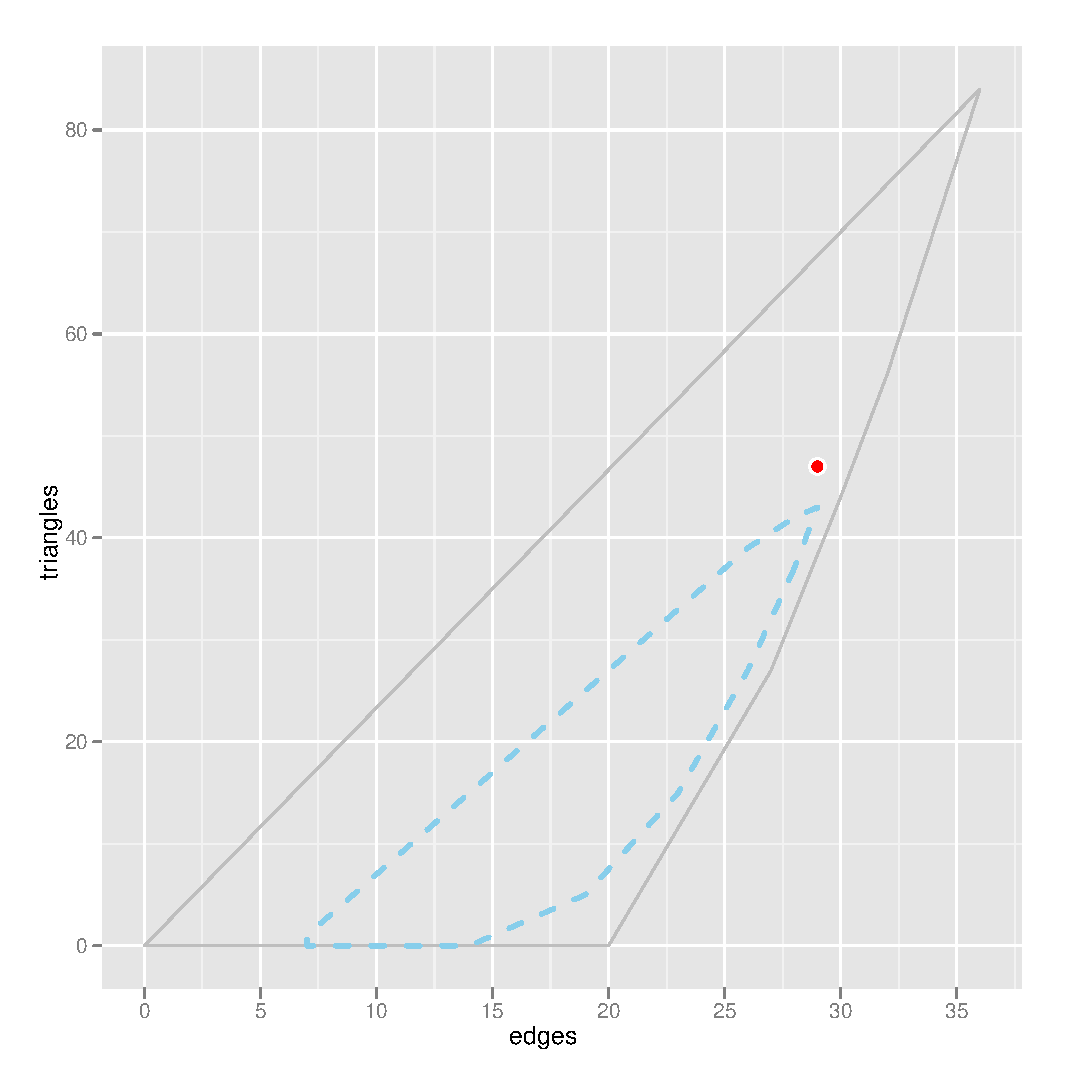
\includegraphics[height=2.8in,width=2.8in]{Figures/MCsample-far}
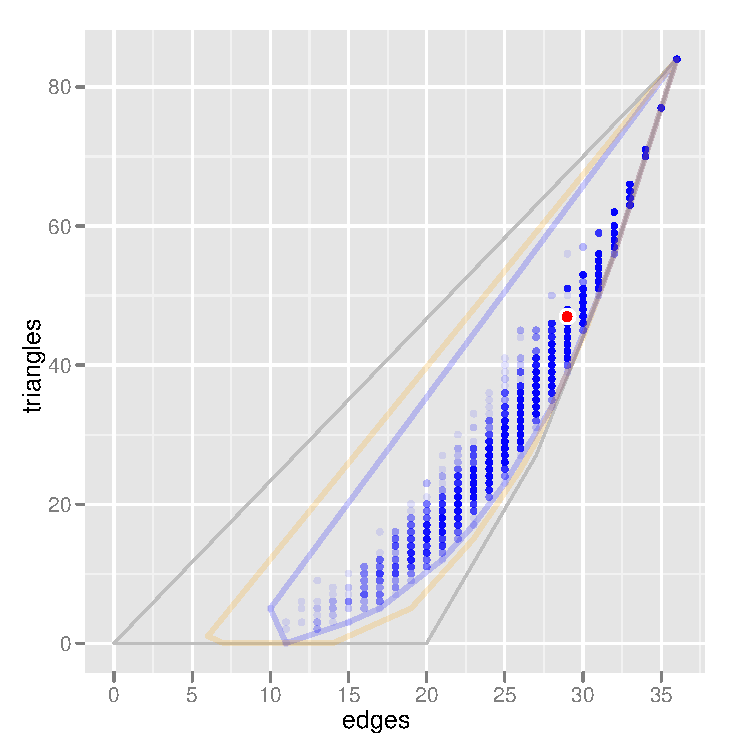
\includegraphics[height=2.8in,width=2.8in]{Figures/MCsample-MLE}
\caption{The network statistics for 10,000 Monte Carlo samples generated from models 
with the natural parameter $\eta$ set to $(0,0)$ (top) and the MLE, $(-0.389, 0.418)$ 
(bottom).  The observed data has network statistics of $(29,47)$, depicted by the 
larger point with white outline.  When $\eta$ is the MLE, the observed statistic is 
exactly the mean of the MC sample points generated from the model with this parameter 
value. }
\label{F:MC cloud}
% (-0.3890151, 0.4177752)
\end{figure}
For this problem, the MLE for $\eta$ is found to be
\begin{align*}
\etaMLE = (-0.389, 0.418).
\end{align*}

\subsubsection{Case: MLE does not exist; observed statistic on one-dimensional face}
If the observed data has network statistic $(31,50)$ and lies on the 
boundary of the convex support as depicted in Figure \ref{F:MC face}, the MLE does not 
exist.  To be precise, the observed network statistic $(31,50)$ lies on the interior 
of a line segment on the boundary with end points $(30,44)$ and $(32,56)$. 
Our algorithm begins as before, generating MC�sample point clouds to explore the 
sample space, as depicted in Figure \ref{F:MC face}.  Because the sail-shaped convex 
support is not known, the algorithm cannot determine at the outset  that the MLE does 
not exist; it can only generate more sample point clouds as it climbs the log 
likelihood surface, with successive clouds moving towards the observed statistic.
Eventually, the observed statistic will lie exactly on the boundary of a sample cloud.  
When this occurs, the algorithm must 
\begin{enumerate}
\item determine empirically the face, $F$, on which the observed statistic lies in the 
relative interior of,
\item decide if $F$ is in fact the boundary of the convex support $C$.
\end{enumerate}  

The first task can be done using the linear programming functions provided to us in 
the \texttt{rcdd} package.  The second task turns out to be very difficult to do.  
For now, we assume that if a substantial portion of the sample points generated, say 
60\%, land on this empirically determined face $F$, then it is in fact a boundary of 
the convex support $C$.  


In this example, the algorithm has determined empirically that $(30,44)$, $(31,50)$, 
and $(32,56)$ lie on a one-dimensional face, as depicted in Figure \ref{F:MC face} 
(bottom).  If less than 60\% of the sample points land on this empirical face, the 
algorithm continues to sample, trying to get a sample point cloud even closer to the 
observed statistic.  We choose such a high proportion for a cut off to eliminate---or 
at least, greatly reduce---the possibility of misidentifying a boundary.
(We deal later with a case where 100\% of the MC sample points form a face which is 
\emph{not} on the boundary of $C$.)
\begin{figure}[!ht]
\centering
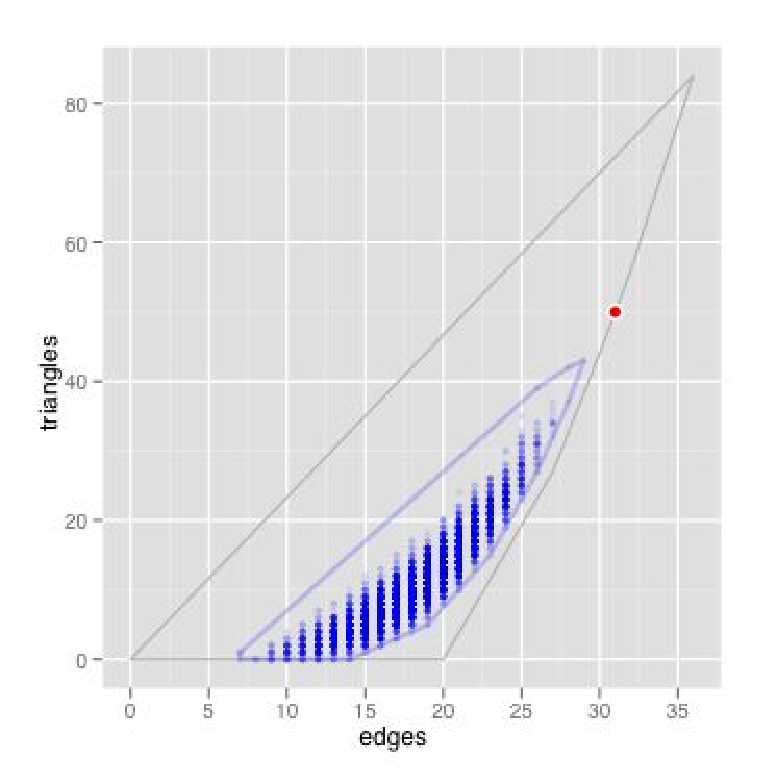
\includegraphics[height=2.7in,width=2.7in]{Figures/MCsample-boundary}
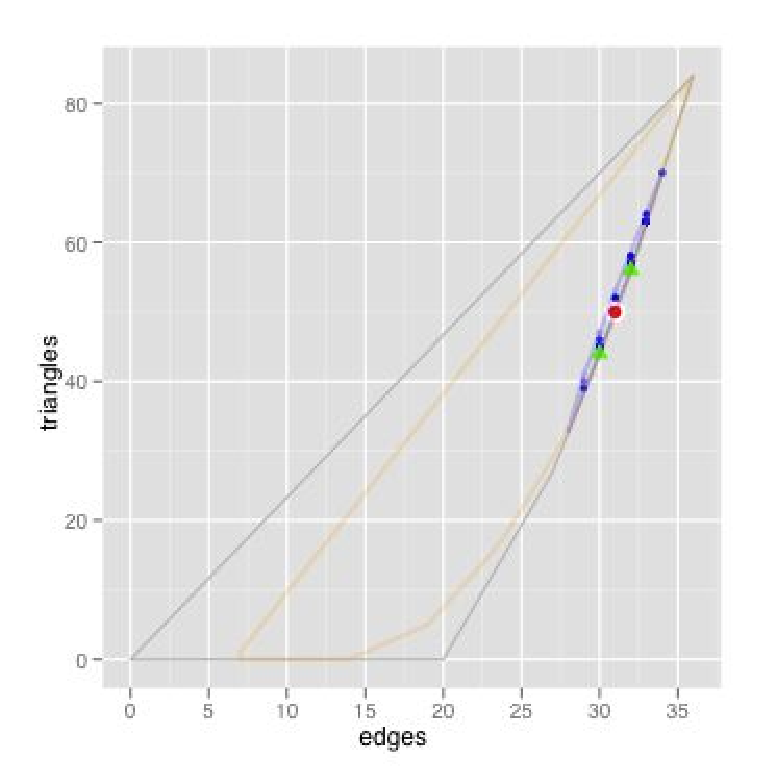
\includegraphics[height=2.7in,width=2.7in]{Figures/MCsample-77face}
\caption{The network statistics for 10,000 Monte Carlo samples for the model with 
observed network statistic $(31,50)$, depicted by the larger point with white 
outline, lying on the boundary of the convex support (top).
In the bottom figure, the algorithm has identified a face defined by $(30,44)$, 
$(31,50)$, and $(32,56)$, marked by triangles in the figure (the triangle for 
$(31,50)$ is not visible since it is the observed statistic).  
Here, 77\% of the MC sample points fall on these three points.  The 
lighter colored polytope is the convex hull of all previously sampled points.
}
\label{F:MC face}
\end{figure}

By identifying the empirical face $F$ on whose interior the observed statistic lies, 
the algorithm has not only concluded that the MLE does not exist in the conventional 
sense, it has also defined $F$ as the convex support for the new limiting conditional 
model, which is also an exponential family.  

The algorithm proceeds to maximize this new exponential family using the same 
iterative approach as before.  The gradient of the LCM log likelihood is approximated 
using \eqref{E:nabla ell approx LCM},
\begin{align*}
	\nabla \ell( \eta )^{LCM} \approx g(\yobs) - \frac{1}{k} \sum_{i=1}^k g(Y_{(k)})
\end{align*}
where $g(Y_{(1)}), \ldots, g(Y_{(k)})$ is the subsample of the MC sample points 
restricted to the empirical face: $(30,44)$, $(31,50)$, and $(32,56)$ in this case.  
The maximizer of this log likelihood, $\etaLCM$, is found to be
\begin{align*}
\etaLCM = (120.9, -20.1).
%(120.91090 -20.12784)
\end{align*}
The LCM, however, is not identifiable, since the support is now only one-dimensional 
compared to two in the original model (EXPLAIN BETTER).  
That is, there must exist a constancy space of this new model, $\Gammalim$, such that 
\begin{align} \label{E:Gammalim}
\ell( \eta + \gamma )^{LCM} = \ell( \eta )^{LCM}
\end{align}
for any $\gamma \in \Gammalim$.

The empirical face $F$ and the observed statistic also define a normal cone, which in this case is a single direction, 
\begin{align*}
	\delta = (6,-1),
\end{align*}
which is called a generic direction of recession (GDOR).  Exponential family theory 
states that the log likelihood is a strictly concave function of $\eta$.  For a 
maximizer to exist then, there must be a direction along which the log likelihood 
function increases to $+\infty$.  This direction is exactly the $\delta$ found above, 
and combined with a specific point in the natural parameter space, $\etaLCM$, 
\begin{align} \label{E:GDOR lim}
	\lim_{s \to +\infty} \ell( \etaLCM + s \delta) = \sup_{\eta} \ell(\eta),
\end{align}
where  $\ell(\cdot)$ is the log likelihood of our original model.

The GDOR, $\delta$, of the original model is also a direction of constancy the new 
model.  
Then by \eqref{E:Gammalim} and \eqref{E:GDOR lim}, note that $\ell(\etaLCM + \gamma + 
s \delta)$ goes off to $+\infty$ as $s$ increases.  
In order to construct a one-sided confidence intervals, we need to find the value of 
$s$ for which the probability that the distribution allocates to the event that a 
sample falls on the face of interest is 5\%, that is,
\begin{align*}
P_{\etaLCM + \gamma + s \delta}(g(Y) \in F ) = 0.05.
\end{align*}
Although we cannot evaluate the probability function above, we can generate MC samples 
of $g(Y_1), \ldots, g(Y_m)$ from the distribution with parameter $\etaLCM + \gamma + s 
\delta$ and see for what value of $s$, 5\% of the sample lies in the empirical face we 
found.  

Some numerical work shows that for $\eta = (9.19, -1.51)$, we get 5\% of the MC sample 
on this face.  Or, in terms of non-simultaneous 95\% confidence intervals for the 
components of $\eta$,
\begin{align*}
	[9.19, +\infty)\\
	(-\infty, -1.51],
\end{align*}
where the direction of the interval for the second component is flipped because the 
second component of $\delta$ is negative.

\textbf{Mean value parameters? Are they any more interpretable here?  nice pictures}

%Because our sample space for graphs is still manageable at 69 billion points, we can 
%in fact use numerical optimization methods like trust (CITE?) on the original log 
%likelihood, passing in first and second derivative functions.  Depending on the 
%settings for tolerance, we can get a trust routine to return to what it thinks is an 
%MLE,  
%\begin{align*}
% 	\hat{\eta}_{\textrm{trust}} = (135.6, -22.6),
% \end{align*}
%which are well within our confidence intervals.

%%%%%%%%%%%%%%%%%%%%%%%%%%%%%%%%%%%%%%%%%%%%%%%%%%%%%
\subsubsection{Case: MLE does not exist; observed statistic on zero-dimensional face}
If the observed data has network statistic $(27, 27)$, the point is an extreme point 
of the convex support $C$ (it is a square point on the boundary of the sail in Figure~
\ref{F:g9-hull}) and the MLE does not exist.  In this case, the point itself is the 
face with zero-dimension.  The algorithm proceeds as before, and concludes that the 
point $(27,27)$ is the empirical face $F$ and on the boundary of the hull.
In this case, the limiting conditioning model is completely unidentifiable, and thus 
any value for $\eta$ will be a maximizer.  Our particular implementation found that
\begin{align*}
	\etaLCM = (94.0, -20.4 ).
\end{align*}
The normal cone to the observed statistic in this case is two-dimensional, bounded by 
two vectors,
\begin{align*}
	 \{ (3.857,   -1),	(5.667,   -1) \}.
\end{align*}
If we choose the average of these two vectors, $\delta = (4.76, -1)$, and proceed as 
before, then we find 95\% one-sided confidence intervals for $\eta$ of 
\begin{align*}
%14.495152 -3.703202 
	[14.5, +\infty)\\
	(-\infty, -3.7],
\end{align*}

\textbf{MEAN VALUE PARAMETERS?}


%%%%%%%%%%%%%%%%%%%%%%%%%%%%%%%%%%%%%%%%%%%%%%%%%%%%%
\subsubsection{Case: MLE exists but observed statistic is very near boundary}
If the observed data has network statistic $(21, 4)$, it is in fact on the interior of 
the convex support and so the MLE exists.  
The approaches of \citet{Handcock:degeneracy} and \citet{Rinaldo:2009} would have 
noted that from a mean value pararmeter perspective, this observed statistic likely 
corresponds to a degenerate distribution. The Shannon entropy function would show this 
point to have extremely small entropy, corresponding to a model that puts most of its 
probability on very few points.

The log likelihood for this model is extremely flat, causing some disagreement among 
numerical optimization routines for MLE estimates, though log likelihood values are nearly 
identical.  Using a trust optimization routine we calculate that 
\begin{align*}
%$(24.44, ?6.65)$ from optim.
\etaMLE = (28.86, -7.76).
\end{align*}
The most problematic aspect of this model for us here, however, is that our algorithm 
concludes---incorrectly, of course---that the MLE does not exist, and proceeds to 
calculate the MLE of an LCM.

How does this happen?

Our algorithm begins in the same manner as described previously.  As the algorithm 
proceeds uphill on the log likelihood function, it will iterate $\eta_k$ to a value 
(for example, $(35.34, -9.56)$) where all 10,000 MC sample points generated from the 
model with this parameter value fall on the six points on the line segment between 
$(20,0)$ and $(25,5)$, as depicted in Figure~\ref{F:MC problem}.  The observed value $
(21,4)$ is one of these six points.
In order for the algorithm to have correctly identified the boundary here and conclude 
that $(21,4)$ was on the interior, the extreme point $(27,27)$ would need to have 
occurred in the MC sample.  However, for the parameter value that we consider, model 
assigns a probability of 0.000032 to this point.  Even the MLE model only assigns a 
probability of about 0.00045 to this point.  So, the extreme point that is critical 
for fully determining the convex support is in fact assigned very low probability by 
the MLE model.

\begin{figure}[!h]
\centering
%%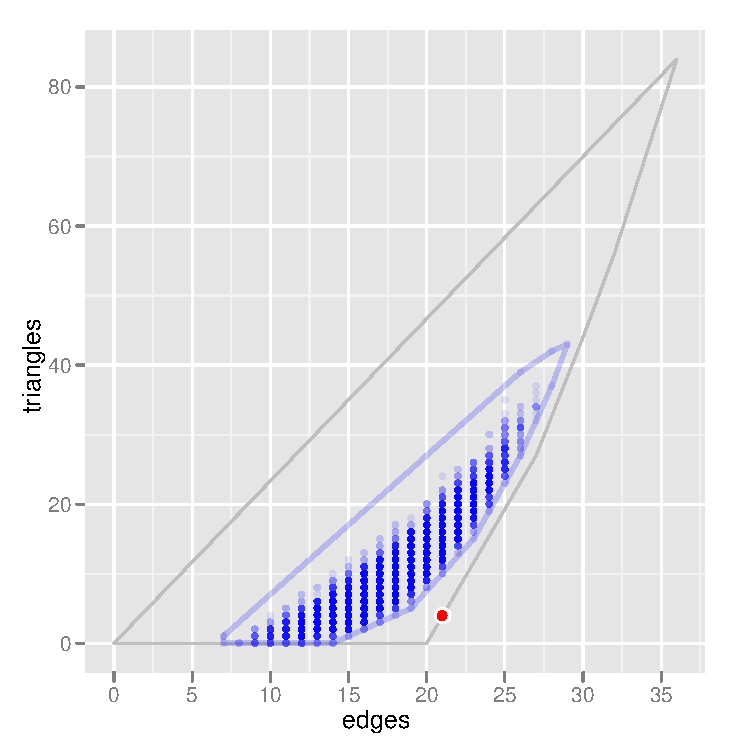
\includegraphics[height=2.4in,width=2.4in]{Figures/MCsample-problem}
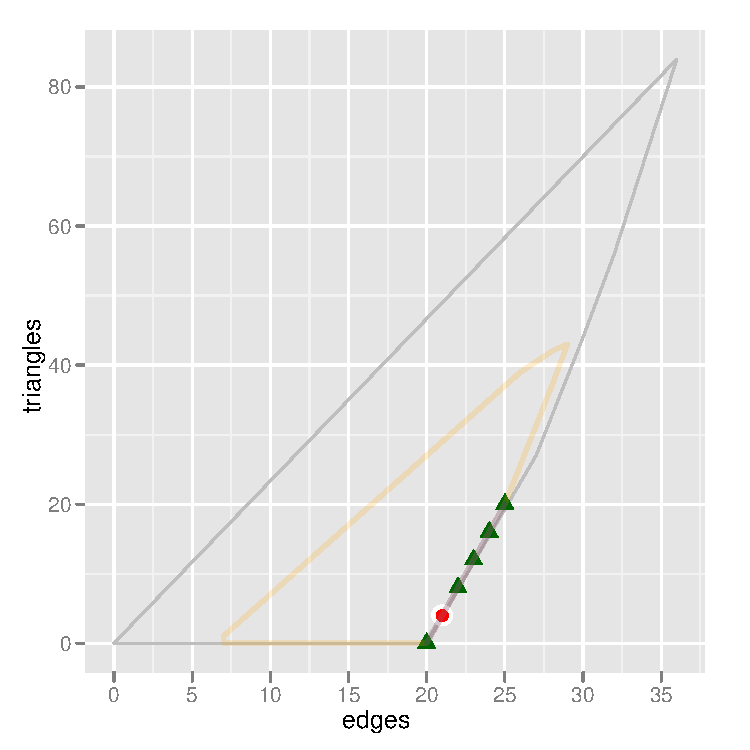
\includegraphics[height=4.5in,width=4.5in]{Figures/MCsample-fakeface}
\caption{An observed statistic at $(21,4)$, in the interior of the convex hull but 
close to the boundary.  It is quite feasible to generate 10,000 MC 
samples where all 10,000 points lie on a line that appear to be a one-dimensional 
face, marked by the 
triangles in the figure above.  The lighter colored polytope is the convex hull of all 
previously 
sampled points used to derive this empirical face.}
\label{F:MC problem}
\end{figure}

According to the algorithm, this line segment is a boundary of the convex support on 
which the observed statistic lies on the interior of, and the MLE does not exist.  It 
proceeds as in the first example, and seeks to find the MLE of the LCM,
\begin{align*}
	\etaLCM = (35.38, -9.39),
\end{align*}
and then calculates one-sided confidence intervals for $\eta$.

On first glance this is very troubling: our algorithm arrives at the wrong conclusion 
about the existence of the MLE, and $(35.38, -9.39)$ does not look particularly close 
to the true MLE of $(28.86, -7.76)$.  However, we believe a step back needs to be 
taken and the goal of the analysis reconsidered.  What was the purpose in finding the 
MLE?  In particular, what does one do with these numbers once they are found?

If the end goal is to try to interpret meaning out of these numbers by their sign and  
magnitude (\textbf{a questionable approach?  or at least dangerous?}), then we indeed 
have a problem---our numbers are just wrong.  However, if the MLE is viewed as an 
index into a specific model that assigns the highest probability to the observed data,
then we claim that the model we have found---the LCM with parameter value $\etaLCM$---
is in fact remarkably similar to the original model indexed by the true MLE.  A 
reasonable metric for this comparison is a sum of the absolute difference in 
probabilities assigned to each point in the sample space,
\begin{align*}
	\sum_{y \in \YY} \abs{ P_{\etaMLE}(g(Y) =g(y) ) -  P_{\etaLCM}(g(Y) = g(y))  }.
\end{align*}
The probabilities assigned by each of these models to the six points on the 
empirically determined face is summarized in Table~\ref{T:LCMvsMLE}.

% latex table generated in R 2.11.1 by xtable 1.5-6 package
% Fri Sep 10 13:22:25 2010
\begin{table}[h!] \label{T:LCMvsMLE}
\begin{center}
\caption{Probabilities assigned by LCM model with parameter value $\etaLCM$ and 
original model with parameter value $\etaMLE$ to six points on empirical face.  The 
observed statistic is $(21,4)$.}

\begin{tabular}{rrrrr}
\\  \hline
 & Edges & Triangles & LCM & MLE \\ 
  \hline
1 & 20 & 0 & 0.3414 & 0.3425 \\ 
  2 & 22 & 8 & 0.2019 & 0.2009 \\ 
  3 & 21 & 4 & 0.3914 & 0.3911 \\ 
  4 & 23 & 12 & 0.0566 & 0.0561 \\ 
  5 & 24 & 16 & 0.0081 & 0.0080 \\ 
  6 & 25 & 20 & 0.0005 & 0.0005 \\ 
   \hline
   &  &  & 1.0000 & 0.9990 \\ 
\end{tabular}
\end{center}
\end{table}

Here, the sum of the absolute value of differences on these empirical points is only 
$0.0031$.  Including the additional 0.001 of probability on points that are outside 
the LCM support, this total still only comes to $0.0041$, a difference that would seem 
insignificant for most applications.  

Of course, there may be practical issues: a researcher may want software to simply 
return MLE values to keep around for later analysis.  Here, we are suggesting the 
analysis return LCM MLE values and an LCM model (perhaps in the form of the convex 
support).  The researcher may understandably be confused, especially if he knew in 
advance that the MLE was guaranteed to exist.  However, any analysis (other than the 
parameter value magnitude study) would still work as before, though perhaps not ``out 
of the box".

It may be of interest to note that $\etaLCM$ and $\etaMLE$ index nearly identical 
models in the LCM, with the difference due almost entirely to the lack of 
identifiability of the LCM.  A normal direction to the empirical face is $\delta = 
(4,-1)$, which is a direction of constancy for the LCM (that is, $\delta \in \Gammalim
$).  Then by \eqref{E:Gammalim}, 
\begin{align*}
	\ell(\etaLCM)^{LCM} &= \ell( \etaLCM + \gamma )^{LCM}\\
				 &= 	\ell(\etaLCM + k \, (4,-1))^{LCM}.
\end{align*}
If we had perfect knowledge and chose $k = -1.63$,
\begin{align*}
	\etaLCM  -1.63 \, (4,-1)= (28.86, -7.76) 
\end{align*}
matching the MLE to the significant figures considered.  Thus in this case, $\etaLCM$ 
and $\etaMLE$ index nearly identical models of the LCM.

If we finished the analysis as before and computed one-sided 95\% confidence intervals 
for $\eta$, we get 
\begin{align*}
%14.495152 -3.703202 
	[20.46, +\infty)\\
	(-\infty, -4.85].
\end{align*}
%20.462923 -4.850603 

%\begin{align*}
%	\hat{\theta}_{MLE} &= (28.85685, -7.75672)\\
%	\hat{\theta}_{LCM} &= (35.3831787, -9.387266),
%\end{align*}

%Well, remember that for LCM's we are looking to construct one-sided CIs.  But here, 
%what happens if we go off to infinity in this supposed direction of recession?  The 
%log-likelihood will eventually dip back down!  So, we can constructed two-sided CI's, 
%I think.  But, my calculations got me something that seems pointlessly wide: 
%\begin{align*}
% (3.503179,  -1.417266 )\\
% (71.22318,  -18.34727 ).
%\end{align*}

%%%%%%%%%%%%%%%%%%%%%%%%%%%%%%%%%%%%%%%%%%%%%%%%%%%%%


\subsection{Three-dimensional sufficient statistic}

In order to increase the complexity of the problem yet still have the ``truth" for 
comparison, we also considered 7-node graph with network statistics edges, two-stars, 
and triangles, a classic model in the literature first suggested by \citet{Frank:
1986}.  Since then it has been criticized for its problematic behavior by \citet
[really? check this]{GOF}, precisely related to the issue of non-existence MLEs (or 
degeneracy???).

The algorithm proceeds in exactly the same way, the difference now being that the 
empirical face may have as many as two dimensions instead of one.  This makes for a 
more interesting variety of constancy spaces for the LCM.  We only consider cases here 
that add a notably different flavor than the two-dimensional case.

\subsubsection{Observed value, $y_{obs}$, is on two-dimensional face}
\subsubsection{Observed value, $y_{obs}$, is on one-dimensional face}
\subsubsection{MLE does not exist; observed statistic on two-dimensional face but not 
fully discoverd}

Set $y_{obs} = (14, 8, 43).$
This point is on the boundary, which is a 2-dim face.

The MC sample, however, does not cover the entire face.  This is a new scenario, but 
it should not be a problem.  Those points on the actual face that are not included are 
simply points of low probability.

Only issue outstanding with this is how long it takes to find the LCM MLE.  Having a 
surprisingly hard time with this.  Question: is it doing any worse than when we 
started with a 2-dim sample space?

\section{Example: \textit{e. coli}?}
\section{Example: Faux Magnolia High School?}
\citet{advancesp*,statnet-tutorial} utilize a adolescent friendship network data set 
of 1,461 students in grade 7--12 derived from the National Longitudinal Study of 
Adolescent Health.  The data set, which \citeauthor{statnet-tutorial} refer to as Faux 
Magnolia High School, is a model-based simulation from the original data set, where 
the simulation is necessitated to maintain confidentiality.


\chapter{Discussion}
We have presented a simple line search algorithm for finding the MLE of a regular 
exponential family when the MLE 
exists.  The algorithm avoids the trial and error experimentation of tuning parameters 
and starting points commonly associated with optimization routines
not invented by optimization specialists.  Our algorithm is modeled after algorithms 
discussed in optimization textbooks \citep{Fletcher,NW,Sun:2006},
all of which are safeguarded to ensure rapid automatic convergence.
%Because it only relies on first order derivatives, this approach avoids problems with 
%near-singular Fisher information 
%matrices that plague methods like Newton-Raphson.  The reliant on a curvature 
%condition for step size makes it less 
%sensitive to poor initial values that are problematic for MCMC-MLE and  SA in 
practice.

Convergence is guaranteed when the gradient can be calculated exactly.  Even when the 
gradient cannot be calculated 
exactly and is only estimable via MCMC, the algorithm is still useful in practice, as 
demonstrated by the Ising model 
example.  We have also described a way to construct and use confidence intervals to 
make convergence highly probable.

The algorithm can be computationally demanding.  When the current iteration approaches 
the solution, the 
curvature condition for step size becomes more difficult to satisfy and the method may 
require several iterations of 
MCMC sampling and perhaps an increase in MCMC sample size.  Eventual increase in MCMC 
sample size is unavoidable,
because the achievable accuracy is inversely proportional to the square root of the 
MCMC sample size, as in all Monte Carlo.
Thus we believe the best use of this algorithm is in combination with other faster 
methods like MCMC-MLE \citep{Geyer:1992}
or Newton-Raphson safeguarded by our line search algorithm.  Our 
algorithm should be used from ``long range'', when one has no good intuition for an 
initial value and is concerned about 
picking one that is far from the MLE.  The switch between types of search direction 
(steepest ascent, conjugate gradient,
or Newton) within our algorithm or the switch to another algorithm (such as MCMC-MLE 
\citep{Geyer:1992})
need not require manual intervention.  When used in combination in this
manner, we do not think the confidence intervals are necessary as the curvature 
condition is quite easily satisfied 
when the current iteration is far from the MLE.

One way to improve performance is to use conjugate gradient search directions rather 
than steepest ascent.  In our 
examples, this reduced the number of iterations by over 25\%.  However, in other 
problems we tried with different 
dimensionality, this performance varied significantly and it appears that no guarantee 
can be made about quantity of 
improvement in performance, though in all cases we examined, it never did worse.  This 
is no surprise, because the
necessity of ``preconditioning'' for good performance of the conjugate gradient 
algorithm is well known (but 
we know of no literature about ``preconditioners'' for 
for maximum likelihood in exponential families).

There are several outstanding issues.  Most notably, we have not showed convergence of 
the algorithm when the gradient 
is approximated via MCMC.  This is a more difficult theoretical problem and is the 
motivation for stochastic 
approximation research.  
Further work is necessary to determine if one can adapt our restrictive curvature 
condition \eqref{E:Wolfe-ll} to the 
approach of \citet{Andrieu:2005} or \citet{Liang:2010} in MCMC stochastic 
approximation.  

Another remaining issue is the stopping criteria: what value should be chosen for $
\epsilon$ in the exit condition
$\lVert  \nabla \ell( \eta_k ) \rVert < \epsilon$?  Because the value of $\lVert  
\nabla \ell( \eta_k ) \rVert$ can only 
be approximated via MCMC, one cannot be certain if this condition is actually 
satisfied.  Here again, the switch to 
another methodology may be appropriate, though at least in our Ising model example, 
our use of 10,000 for the MCMC 
sample size and 0.005 for $\epsilon$ were successful in obtaining a reasonable 
parameter estimate. 

 A final remaining issue is estimation of Monte Carlo error of the estimates.  Here 
too we recommend switching to another
algorithm at the end.  The MCMC-MLE procedure gives accurate error estimates 
\citep{Geyer:1994}.
For very small steps these are essentially the same as the Monte Carlo error of a 
single unsafeguarded Newton-Raphson step,
so the method in \citep{Geyer:1994} can be used for either.

\section{non-existent MLE}
ALSO.  simulated tempering for faster convergence.

MLE.  What does it mean to ``find the MLE"?


% References don't have to be double spaced either
\setstretch{1.3}
\bibliographystyle{ims}
%\bibliographystyle{imsart-nameyear}
\bibliography{References}
%\bibliography{/Users/saipuck/Tako/THESIS/References}

% text in appendices may be single spaced, if desired
\setstretch{1.3} % to 1.3 spacing
\appendix
\chapter{Brute Force Network Statistic Counting} \label{Section:Count Triangles}
\label{A:Triangle count}
As noted in Section~\ref{S:ERGM setup}, even for an undirected 9-node network, 
there are $2^{{9\choose 2}}$, or about 69 billion different possible graphs.
Counting the network statistics of edges, two-stars, and triangles for this
network is not a trivial calculation and can take an enormous amount of time 
if not coded efficiently (our first straightforward implementation 
entirely in R would have taken over a year).  Thus every effort must 
be made to represent the data as efficiently as possible, 
implementing loops in C and avoiding calculations.

A few quantities are easily obtained: the maximum number of edge is 
${n \choose 2} = {9 \choose 2} = 36$.  The maximum number of triangles is 
${n \choose 3} = {9 \choose 3} = 84$, since a triangle requires 3 of the 9 actors.  
For each triangle, there are 3  different two-stars, so the maximum number 
of two-stars is $3 \cdot 84 = 252$.

%Now, R (and all other programming platforms at the moment) cannot handle $2^{36}$ as an integer; in fact, casting $2^{31}$ as an integer produces an error.  Thus we do not want to write a \texttt{for} loop going from 1 to $2^{36}$.  So what to do?  

The approach we have implemented requires first creating a collection of graphs,
one graph for each possible network structure of interest (triangle or two star),
where each graph is empty except for that particular network structure.  For example,
one graph in this collection is the one representing a triangle between the 1st, 2nd, and 3rd nodes.  In matrix
form, this network has all zeros except for ones in entires of (1,2), (1,3), (2,3), 
(2,1), (3,1), (3,2).
We then compare each of the 69 billion possible graphs to this collection.
Every time a comparison yields a match, that particular configuration is present
and the count for that statistic is incremented by one.  
The reason this is efficient is because we can actually represent the 
a graph as a single binary number and do bitwise comparisons for far greater speed.

We can explain this in further detail with triangles.
We know there are ${9 \choose 3} = 84$ possible triangles, and so we create
84 graphs, each with only one triangle present among 3 actors.  
So, the first element corresponds to a graph with ties present between 
actors 1, 2, and 3, and no other ties present, the second element corresponds 
to a graph with a ties present between actors 1, 2, and 4.  
Because the network is undirected, the adjacency matrix is symmetric and 
can be fully described by just its upper triangle, which in our convention 
of going down vertically and then across is $(1,1,1,0,0,0, \ldots,0)$.  
We can treat this upper triangular vector as a 36-digit number, 
111000000000000000000000000000000000.  If we treat this as a number 
in base 2, we can convert it to base 10 to a number less than $2^{36}$.  
For this first matrix, it is 60,129,542,144.  Proceeding in this manner up 
through 84, we have a set of 84 numbers corresponding to all the possible 
triangle configurations in the network.  

We now turn our attention to iterating through the $2^{36} \approx 69$ billion possible graphs.  
Using the \texttt{long int} representation in C (on a 64-bit system), 
we can in fact iterate from 0 to $2^{36}-1$.  By having the index itself 
correspond to a specific graph,  we can treat its binary form as 
the collapsed upper triangular vector.
For example, the last index corresponding to $2^{36}-1$ has binary form of 
 111111111111111111111111111111111111 which shows every tie present and
 is the complete graph.
   
For each graph index, we can loop through our set of 84 triangle numbers
and perform bitwise logic operations (the \texttt{\&} operator in C) to 
compare the binary form of the graph index to each of the triangle numbers.  
In binary form, if there are ones in all the digits that the triangle number has a 
one in, 
then the graph has this particular triangle present.
For example, the operation $(2^{36}-1)$ \& $60,129,542,144$ would return 
111000000000000000000000000000000000 in binary form, indicating that this 
particular triangle is present.  This is confirmed by comparing the
result of the binary operation back to the original triangle number,
which would return TRUE.  Proceeding through all the other triangle numbers, 
we get a count of how many triangles are present for this graph index.

A similar method is employed for counting two-stars, where we would similarly
first calculate the $3\times84 = 252$ two-stars graph numbers before iterating
through the graph indices.

To count edges, there are well-known tricks to count the number of ones 
in a binary number in C which cleverly use the `\texttt{>>}' shift operator.
By taking the graph index \texttt{>> 1}, it moves all the digits to the 
right by dropping off the rightmost digit and adding a 0 to the 
farthest left digit.  So, 
\begin{align*}
111111111111111111111111111111111111 >> 1
\end{align*}
returns 01111111111111111111111111111111111 (where there are now 35 ones instead of 36).  
In this manner, the shifts can be continued and ones counted 
(done by another bit comparison to '01' using the `\texttt{\&}' again) 
until there are no more ones.  This approach avoids any arithmetic and is thus much faster.  
It should be noted that a computer always stores the \texttt{long int} in binary form 
and so the 36-digit representation used here is entirely for our benefit only.

Finally, we can further speed up the calculations by parallelizing this computation.  
We can count the number of edges, two-stars, and triangles in the 
first $2^{36}/8$ graphs at the same time that we count them in the last $2^{36}/8$ graphs.  
To do this, we simply use the \texttt{mclapply} function in the \texttt{multicore} \citep{multicore:R} 
library in R.
At the time of this writing, we performed this calculation on an 8-CPU 2.9GHz linux box
which took 2 hour 15 minutes to complete.  







\end{document}